\documentclass[a4paper]{book}
\usepackage{makeidx}
\usepackage{natbib}
\usepackage{graphicx}
\usepackage{multicol}
\usepackage{float}
\usepackage{listings}
\usepackage{color}
\usepackage{ifthen}
\usepackage[table]{xcolor}
\usepackage{textcomp}
\usepackage{alltt}
\usepackage{ifpdf}
\ifpdf
\usepackage[pdftex,
            pagebackref=true,
            colorlinks=true,
            linkcolor=blue,
            unicode
           ]{hyperref}
\else
\usepackage[ps2pdf,
            pagebackref=true,
            colorlinks=true,
            linkcolor=blue,
            unicode
           ]{hyperref}
\usepackage{pspicture}
\fi
\usepackage[utf8]{inputenc}
\usepackage{mathptmx}
\usepackage[scaled=.90]{helvet}
\usepackage{courier}
\usepackage{sectsty}
\usepackage[titles]{tocloft}
\usepackage{doxygen}
\lstset{language=C++,inputencoding=utf8,basicstyle=\footnotesize,breaklines=true,breakatwhitespace=true,tabsize=8,numbers=left }
\makeindex
\setcounter{tocdepth}{3}
\renewcommand{\footrulewidth}{0.4pt}
\renewcommand{\familydefault}{\sfdefault}
\hfuzz=15pt
\setlength{\emergencystretch}{15pt}
\hbadness=750
\tolerance=750
\begin{document}
\hypersetup{pageanchor=false,citecolor=blue}
\begin{titlepage}
\vspace*{7cm}
\begin{center}
{\Large \-Ephenation }\\
\vspace*{1cm}
{\large \-Generated by Doxygen 1.7.6.1}\\
\vspace*{0.5cm}
{\small Wed Jan 9 2013 22:22:34}\\
\end{center}
\end{titlepage}
\clearemptydoublepage
\pagenumbering{roman}
\tableofcontents
\clearemptydoublepage
\pagenumbering{arabic}
\hypersetup{pageanchor=true,citecolor=blue}
\chapter{\-Todo \-List}
\label{todo}
\hypertarget{todo}{}

\begin{DoxyRefList}
\item[\label{todo__todo000005}%
\hypertarget{todo__todo000005}{}%
\-Class \hyperlink{classQuad}{\-Quad} ]\-Why not inherit from \hyperlink{classShaderBase}{\-Shader\-Base}?  
\item[\label{todo__todo000001}%
\hypertarget{todo__todo000001}{}%
\-Class \hyperlink{classShaderBase}{\-Shader\-Base} ]use link, link from main page?  
\item[\label{todo__todo000004}%
\hypertarget{todo__todo000004}{}%
\-Class \hyperlink{classSkyBox}{\-Sky\-Box} ]\-: explain above better. 
\item[\label{todo__todo000002}%
\hypertarget{todo__todo000002}{}%
\-File \hyperlink{skybox_8cpp}{skybox.cpp} ]\mbox{[}position = pos$\ast$10000\mbox{]}  
\item[\label{todo__todo000003}%
\hypertarget{todo__todo000003}{}%
\-Member \hyperlink{classSkyBox_ab9db46f2e34683cae517ba97a44aee9e}{\-Sky\-Box\-:\-:\-Draw} ()]\-Move the model transforms to shader? 
\end{DoxyRefList}
\chapter{\-Class \-Index}
\section{\-Class \-Hierarchy}
\-This inheritance list is sorted roughly, but not completely, alphabetically\-:\begin{DoxyCompactList}
\item \contentsline{section}{\-Blender\-Model\-:\-:\-Animation}{\pageref{structBlenderModel_1_1Animation}}{}
\item \contentsline{section}{\-Animation\-Bone}{\pageref{structAnimationBone}}{}
\item \contentsline{section}{\-Animation\-Models}{\pageref{classAnimationModels}}{}
\item \contentsline{section}{\-Billboard}{\pageref{classBillboard}}{}
\item \contentsline{section}{\-Blender\-Model}{\pageref{classBlenderModel}}{}
\item \contentsline{section}{\-Building\-Blocks}{\pageref{classBuildingBlocks}}{}
\item \contentsline{section}{\-Chunk\-Cache\-:\-:cachunk}{\pageref{structChunkCache_1_1cachunk}}{}
\item \contentsline{section}{chunk}{\pageref{structchunk}}{}
\item \contentsline{section}{\-Chunk\-Blocks}{\pageref{structChunkBlocks}}{}
\item \contentsline{section}{\-Chunk\-Cache}{\pageref{classChunkCache}}{}
\item \contentsline{section}{\-Chunk\-Coord}{\pageref{structChunkCoord}}{}
\item \contentsline{section}{\-Chunk\-Dist}{\pageref{structChunkDist}}{}
\item \contentsline{section}{\-Super\-Chunk\-:\-:chunk\-Info}{\pageref{structSuperChunk_1_1chunkInfo}}{}
\item \contentsline{section}{\-Chunk\-Object}{\pageref{classChunkObject}}{}
\item \contentsline{section}{\-Chunk\-Offset\-Coord}{\pageref{structChunkOffsetCoord}}{}
\item \contentsline{section}{\-Chunk\-Process}{\pageref{classChunkProcess}}{}
\item \contentsline{section}{\-Compare\-Vertex\-Dataf}{\pageref{structCompareVertexDataf}}{}
\item \contentsline{section}{std\-:\-:condition\-\_\-variable}{\pageref{classstd_1_1condition__variable}}{}
\item \contentsline{section}{\-Cube}{\pageref{classCube}}{}
\item \contentsline{section}{\-Cylinder}{\pageref{classCylinder}}{}
\item \contentsline{section}{\-Data}{\pageref{structData}}{}
\item \contentsline{section}{\-Draw\-Font}{\pageref{classDrawFont}}{}
\item \contentsline{section}{\-Draw\-Object\-List}{\pageref{structDrawObjectList}}{}
\item \contentsline{section}{\-Draw\-Texture}{\pageref{classDrawTexture}}{}
\item \contentsline{section}{\-Fogs}{\pageref{classFogs}}{}
\item \contentsline{section}{game\-Dialog}{\pageref{classgameDialog}}{}
\item \contentsline{section}{\-Game\-Mode}{\pageref{classGameMode}}{}
\item \contentsline{section}{\-Game\-Texture}{\pageref{structGameTexture}}{}
\item \contentsline{section}{\-Health\-Bar}{\pageref{classHealthBar}}{}
\item \contentsline{section}{\-Image}{\pageref{classImage}}{}
\item \contentsline{section}{\-Inventory}{\pageref{classInventory}}{}
\item \contentsline{section}{\-Inventory\-:\-:\-Item}{\pageref{structInventory_1_1Item}}{}
\item \contentsline{section}{\-Chunk\-Blocks\-:\-:\-Jelly\-Block}{\pageref{structChunkBlocks_1_1JellyBlock}}{}
\item \contentsline{section}{\-Map}{\pageref{classMap}}{}
\item \contentsline{section}{\-Blender\-Model\-:\-:\-Mesh}{\pageref{structBlenderModel_1_1Mesh}}{}
\item \contentsline{section}{\-Mesh\-Bone}{\pageref{structMeshBone}}{}
\item \contentsline{section}{\-Scrolling\-Messages\-:\-:\-Message}{\pageref{structScrollingMessages_1_1Message}}{}
\item \contentsline{section}{\-Monsters}{\pageref{classMonsters}}{}
\item \contentsline{section}{\-Msg\-Window}{\pageref{classMsgWindow}}{}
\item \contentsline{section}{std\-:\-:mutex}{\pageref{classstd_1_1mutex}}{}
\item \contentsline{section}{\-Object}{\pageref{classObject}}{}
\begin{DoxyCompactList}
\item \contentsline{section}{player}{\pageref{classplayer}}{}
\end{DoxyCompactList}
\item \contentsline{section}{\-Inventory\-:\-:\-Object\-Map}{\pageref{structInventory_1_1ObjectMap}}{}
\item \contentsline{section}{\-Options}{\pageref{classOptions}}{}
\item \contentsline{section}{\-Other\-Players}{\pageref{classOtherPlayers}}{}
\item \contentsline{section}{\-Picking\-Data}{\pageref{unionPickingData}}{}
\item \contentsline{section}{\-Quad}{\pageref{classQuad}}{}
\item \contentsline{section}{\-Quad\-Stage1}{\pageref{classQuadStage1}}{}
\item \contentsline{section}{\-Render\-Control}{\pageref{classRenderControl}}{}
\item \contentsline{section}{\-Scrolling\-Messages}{\pageref{classScrollingMessages}}{}
\item \contentsline{section}{\-Shader\-Base}{\pageref{classShaderBase}}{}
\begin{DoxyCompactList}
\item \contentsline{section}{\-Add\-Dynamic\-Shadow}{\pageref{classAddDynamicShadow}}{}
\item \contentsline{section}{\-Add\-Local\-Fog}{\pageref{classAddLocalFog}}{}
\item \contentsline{section}{\-Add\-Point\-Light}{\pageref{classAddPointLight}}{}
\item \contentsline{section}{\-Add\-Point\-Shadow}{\pageref{classAddPointShadow}}{}
\item \contentsline{section}{\-Add\-S\-S\-A\-O}{\pageref{classAddSSAO}}{}
\item \contentsline{section}{\-Chunk\-Shader\-Picking}{\pageref{classChunkShaderPicking}}{}
\item \contentsline{section}{\-Color\-Shader}{\pageref{classColorShader}}{}
\item \contentsline{section}{\-Deferred\-Lighting}{\pageref{classDeferredLighting}}{}
\item \contentsline{section}{\-Modulated\-Texture\-Shader}{\pageref{classModulatedTextureShader}}{}
\item \contentsline{section}{\-Monster\-Shader}{\pageref{classMonsterShader}}{}
\item \contentsline{section}{\-Simple\-Texture\-Shader}{\pageref{classSimpleTextureShader}}{}
\item \contentsline{section}{\-Sky\-Box}{\pageref{classSkyBox}}{}
\item \contentsline{section}{\-Stage\-One\-Shader}{\pageref{classStageOneShader}}{}
\begin{DoxyCompactList}
\item \contentsline{section}{\-Animation\-Shader}{\pageref{classAnimationShader}}{}
\item \contentsline{section}{\-Chunk\-Shader}{\pageref{classChunkShader}}{}
\item \contentsline{section}{\-Shadow\-Map\-Shader}{\pageref{classShadowMapShader}}{}
\item \contentsline{section}{\-Transp\-Shader}{\pageref{classTranspShader}}{}
\end{DoxyCompactList}
\end{DoxyCompactList}
\item \contentsline{section}{\-Shadow\-Render}{\pageref{classShadowRender}}{}
\item \contentsline{section}{\-Shadows}{\pageref{classShadows}}{}
\item \contentsline{section}{\-Sound\-Control}{\pageref{classSoundControl}}{}
\item \contentsline{section}{\-Chunk\-Object\-:\-:\-Special\-Object}{\pageref{structChunkObject_1_1SpecialObject}}{}
\item \contentsline{section}{\-Splitter}{\pageref{classSplitter}}{}
\item \contentsline{section}{\-Super\-Chunk}{\pageref{structSuperChunk}}{}
\item \contentsline{section}{\-Super\-Chunk\-Manager}{\pageref{classSuperChunkManager}}{}
\item \contentsline{section}{std\-:\-:thread}{\pageref{classstd_1_1thread}}{}
\item \contentsline{section}{\-Time\-Measure}{\pageref{classTimeMeasure}}{}
\item \contentsline{section}{\-Tree}{\pageref{classTree}}{}
\item \contentsline{section}{\-Triangle\-Surfacef}{\pageref{structTriangleSurfacef}}{}
\item \contentsline{section}{\-Sound\-Control\-:\-:\-Trig\-Sound\-Item}{\pageref{structSoundControl_1_1TrigSoundItem}}{}
\item \contentsline{section}{\-T\-S\-Exec}{\pageref{classTSExec}}{}
\item \contentsline{section}{\-Uniform\-Buffer}{\pageref{classUniformBuffer}}{}
\item \contentsline{section}{std\-:\-:unique\-\_\-lock$<$ \-T $>$}{\pageref{classstd_1_1unique__lock}}{}
\item \contentsline{section}{vertex}{\pageref{structvertex}}{}
\item \contentsline{section}{\-Vertex\-Dataf}{\pageref{structVertexDataf}}{}
\item \contentsline{section}{\-Worst\-Time}{\pageref{classWorstTime}}{}
\end{DoxyCompactList}

\chapter{\-Class \-Index}
\section{\-Class \-List}
\-Here are the classes, structs, unions and interfaces with brief descriptions\-:\begin{DoxyCompactList}
\item\contentsline{section}{\hyperlink{classAddDynamicShadow}{\-Add\-Dynamic\-Shadow} }{\pageref{classAddDynamicShadow}}{}
\item\contentsline{section}{\hyperlink{classAddLocalFog}{\-Add\-Local\-Fog} }{\pageref{classAddLocalFog}}{}
\item\contentsline{section}{\hyperlink{classAddPointLight}{\-Add\-Point\-Light} }{\pageref{classAddPointLight}}{}
\item\contentsline{section}{\hyperlink{classAddPointShadow}{\-Add\-Point\-Shadow} }{\pageref{classAddPointShadow}}{}
\item\contentsline{section}{\hyperlink{classAddSSAO}{\-Add\-S\-S\-A\-O} }{\pageref{classAddSSAO}}{}
\item\contentsline{section}{\hyperlink{structBlenderModel_1_1Animation}{\-Blender\-Model\-::\-Animation} }{\pageref{structBlenderModel_1_1Animation}}{}
\item\contentsline{section}{\hyperlink{structAnimationBone}{\-Animation\-Bone} }{\pageref{structAnimationBone}}{}
\item\contentsline{section}{\hyperlink{classAnimationModels}{\-Animation\-Models} }{\pageref{classAnimationModels}}{}
\item\contentsline{section}{\hyperlink{classAnimationShader}{\-Animation\-Shader} }{\pageref{classAnimationShader}}{}
\item\contentsline{section}{\hyperlink{classBillboard}{\-Billboard} }{\pageref{classBillboard}}{}
\item\contentsline{section}{\hyperlink{classBlenderModel}{\-Blender\-Model} }{\pageref{classBlenderModel}}{}
\item\contentsline{section}{\hyperlink{classBuildingBlocks}{\-Building\-Blocks} }{\pageref{classBuildingBlocks}}{}
\item\contentsline{section}{\hyperlink{structChunkCache_1_1cachunk}{\-Chunk\-Cache\-::cachunk} }{\pageref{structChunkCache_1_1cachunk}}{}
\item\contentsline{section}{\hyperlink{structchunk}{chunk} }{\pageref{structchunk}}{}
\item\contentsline{section}{\hyperlink{structChunkBlocks}{\-Chunk\-Blocks} }{\pageref{structChunkBlocks}}{}
\item\contentsline{section}{\hyperlink{classChunkCache}{\-Chunk\-Cache} }{\pageref{classChunkCache}}{}
\item\contentsline{section}{\hyperlink{structChunkCoord}{\-Chunk\-Coord} }{\pageref{structChunkCoord}}{}
\item\contentsline{section}{\hyperlink{structChunkDist}{\-Chunk\-Dist} }{\pageref{structChunkDist}}{}
\item\contentsline{section}{\hyperlink{structSuperChunk_1_1chunkInfo}{\-Super\-Chunk\-::chunk\-Info} }{\pageref{structSuperChunk_1_1chunkInfo}}{}
\item\contentsline{section}{\hyperlink{classChunkObject}{\-Chunk\-Object} }{\pageref{classChunkObject}}{}
\item\contentsline{section}{\hyperlink{structChunkOffsetCoord}{\-Chunk\-Offset\-Coord} }{\pageref{structChunkOffsetCoord}}{}
\item\contentsline{section}{\hyperlink{classChunkProcess}{\-Chunk\-Process} }{\pageref{classChunkProcess}}{}
\item\contentsline{section}{\hyperlink{classChunkShader}{\-Chunk\-Shader} }{\pageref{classChunkShader}}{}
\item\contentsline{section}{\hyperlink{classChunkShaderPicking}{\-Chunk\-Shader\-Picking} }{\pageref{classChunkShaderPicking}}{}
\item\contentsline{section}{\hyperlink{classColorShader}{\-Color\-Shader} }{\pageref{classColorShader}}{}
\item\contentsline{section}{\hyperlink{structCompareVertexDataf}{\-Compare\-Vertex\-Dataf} }{\pageref{structCompareVertexDataf}}{}
\item\contentsline{section}{\hyperlink{classstd_1_1condition__variable}{std\-::condition\-\_\-variable} }{\pageref{classstd_1_1condition__variable}}{}
\item\contentsline{section}{\hyperlink{classCube}{\-Cube} }{\pageref{classCube}}{}
\item\contentsline{section}{\hyperlink{classCylinder}{\-Cylinder} }{\pageref{classCylinder}}{}
\item\contentsline{section}{\hyperlink{structData}{\-Data} }{\pageref{structData}}{}
\item\contentsline{section}{\hyperlink{classDeferredLighting}{\-Deferred\-Lighting} }{\pageref{classDeferredLighting}}{}
\item\contentsline{section}{\hyperlink{classDrawFont}{\-Draw\-Font} }{\pageref{classDrawFont}}{}
\item\contentsline{section}{\hyperlink{structDrawObjectList}{\-Draw\-Object\-List} }{\pageref{structDrawObjectList}}{}
\item\contentsline{section}{\hyperlink{classDrawTexture}{\-Draw\-Texture} }{\pageref{classDrawTexture}}{}
\item\contentsline{section}{\hyperlink{classFogs}{\-Fogs} }{\pageref{classFogs}}{}
\item\contentsline{section}{\hyperlink{classgameDialog}{game\-Dialog} }{\pageref{classgameDialog}}{}
\item\contentsline{section}{\hyperlink{classGameMode}{\-Game\-Mode} }{\pageref{classGameMode}}{}
\item\contentsline{section}{\hyperlink{structGameTexture}{\-Game\-Texture} }{\pageref{structGameTexture}}{}
\item\contentsline{section}{\hyperlink{classHealthBar}{\-Health\-Bar} }{\pageref{classHealthBar}}{}
\item\contentsline{section}{\hyperlink{classImage}{\-Image} }{\pageref{classImage}}{}
\item\contentsline{section}{\hyperlink{classInventory}{\-Inventory} }{\pageref{classInventory}}{}
\item\contentsline{section}{\hyperlink{structInventory_1_1Item}{\-Inventory\-::\-Item} }{\pageref{structInventory_1_1Item}}{}
\item\contentsline{section}{\hyperlink{structChunkBlocks_1_1JellyBlock}{\-Chunk\-Blocks\-::\-Jelly\-Block} }{\pageref{structChunkBlocks_1_1JellyBlock}}{}
\item\contentsline{section}{\hyperlink{classMap}{\-Map} }{\pageref{classMap}}{}
\item\contentsline{section}{\hyperlink{structBlenderModel_1_1Mesh}{\-Blender\-Model\-::\-Mesh} }{\pageref{structBlenderModel_1_1Mesh}}{}
\item\contentsline{section}{\hyperlink{structMeshBone}{\-Mesh\-Bone} }{\pageref{structMeshBone}}{}
\item\contentsline{section}{\hyperlink{structScrollingMessages_1_1Message}{\-Scrolling\-Messages\-::\-Message} }{\pageref{structScrollingMessages_1_1Message}}{}
\item\contentsline{section}{\hyperlink{classModulatedTextureShader}{\-Modulated\-Texture\-Shader} }{\pageref{classModulatedTextureShader}}{}
\item\contentsline{section}{\hyperlink{classMonsters}{\-Monsters} }{\pageref{classMonsters}}{}
\item\contentsline{section}{\hyperlink{classMonsterShader}{\-Monster\-Shader} }{\pageref{classMonsterShader}}{}
\item\contentsline{section}{\hyperlink{classMsgWindow}{\-Msg\-Window} }{\pageref{classMsgWindow}}{}
\item\contentsline{section}{\hyperlink{classstd_1_1mutex}{std\-::mutex} }{\pageref{classstd_1_1mutex}}{}
\item\contentsline{section}{\hyperlink{classObject}{\-Object} }{\pageref{classObject}}{}
\item\contentsline{section}{\hyperlink{structInventory_1_1ObjectMap}{\-Inventory\-::\-Object\-Map} }{\pageref{structInventory_1_1ObjectMap}}{}
\item\contentsline{section}{\hyperlink{classOptions}{\-Options} }{\pageref{classOptions}}{}
\item\contentsline{section}{\hyperlink{classOtherPlayers}{\-Other\-Players} }{\pageref{classOtherPlayers}}{}
\item\contentsline{section}{\hyperlink{unionPickingData}{\-Picking\-Data} }{\pageref{unionPickingData}}{}
\item\contentsline{section}{\hyperlink{classplayer}{player} }{\pageref{classplayer}}{}
\item\contentsline{section}{\hyperlink{classQuad}{\-Quad} \\*\-A very minimal shape, drawing a quad from 0 to 1 in x and y. \-A simple quad drawn using \-V\-A\-O and \-V\-B\-O }{\pageref{classQuad}}{}
\item\contentsline{section}{\hyperlink{classQuadStage1}{\-Quad\-Stage1} }{\pageref{classQuadStage1}}{}
\item\contentsline{section}{\hyperlink{classRenderControl}{\-Render\-Control} }{\pageref{classRenderControl}}{}
\item\contentsline{section}{\hyperlink{classScrollingMessages}{\-Scrolling\-Messages} }{\pageref{classScrollingMessages}}{}
\item\contentsline{section}{\hyperlink{classShaderBase}{\-Shader\-Base} \\*\-Matrices used \-Some general info about how matrices are used in \-Ephenation. \-The most important transformation matrices\-: }{\pageref{classShaderBase}}{}
\item\contentsline{section}{\hyperlink{classShadowMapShader}{\-Shadow\-Map\-Shader} }{\pageref{classShadowMapShader}}{}
\item\contentsline{section}{\hyperlink{classShadowRender}{\-Shadow\-Render} }{\pageref{classShadowRender}}{}
\item\contentsline{section}{\hyperlink{classShadows}{\-Shadows} }{\pageref{classShadows}}{}
\item\contentsline{section}{\hyperlink{classSimpleTextureShader}{\-Simple\-Texture\-Shader} }{\pageref{classSimpleTextureShader}}{}
\item\contentsline{section}{\hyperlink{classSkyBox}{\-Sky\-Box} \\*\-Implementation of the \-Skybox used in \-Ephenation }{\pageref{classSkyBox}}{}
\item\contentsline{section}{\hyperlink{classSoundControl}{\-Sound\-Control} }{\pageref{classSoundControl}}{}
\item\contentsline{section}{\hyperlink{structChunkObject_1_1SpecialObject}{\-Chunk\-Object\-::\-Special\-Object} }{\pageref{structChunkObject_1_1SpecialObject}}{}
\item\contentsline{section}{\hyperlink{classSplitter}{\-Splitter} }{\pageref{classSplitter}}{}
\item\contentsline{section}{\hyperlink{classStageOneShader}{\-Stage\-One\-Shader} }{\pageref{classStageOneShader}}{}
\item\contentsline{section}{\hyperlink{structSuperChunk}{\-Super\-Chunk} }{\pageref{structSuperChunk}}{}
\item\contentsline{section}{\hyperlink{classSuperChunkManager}{\-Super\-Chunk\-Manager} }{\pageref{classSuperChunkManager}}{}
\item\contentsline{section}{\hyperlink{classstd_1_1thread}{std\-::thread} }{\pageref{classstd_1_1thread}}{}
\item\contentsline{section}{\hyperlink{classTimeMeasure}{\-Time\-Measure} }{\pageref{classTimeMeasure}}{}
\item\contentsline{section}{\hyperlink{classTranspShader}{\-Transp\-Shader} }{\pageref{classTranspShader}}{}
\item\contentsline{section}{\hyperlink{classTree}{\-Tree} }{\pageref{classTree}}{}
\item\contentsline{section}{\hyperlink{structTriangleSurfacef}{\-Triangle\-Surfacef} }{\pageref{structTriangleSurfacef}}{}
\item\contentsline{section}{\hyperlink{structSoundControl_1_1TrigSoundItem}{\-Sound\-Control\-::\-Trig\-Sound\-Item} }{\pageref{structSoundControl_1_1TrigSoundItem}}{}
\item\contentsline{section}{\hyperlink{classTSExec}{\-T\-S\-Exec} }{\pageref{classTSExec}}{}
\item\contentsline{section}{\hyperlink{classUniformBuffer}{\-Uniform\-Buffer} }{\pageref{classUniformBuffer}}{}
\item\contentsline{section}{\hyperlink{classstd_1_1unique__lock}{std\-::unique\-\_\-lock$<$ T $>$} }{\pageref{classstd_1_1unique__lock}}{}
\item\contentsline{section}{\hyperlink{structvertex}{vertex} }{\pageref{structvertex}}{}
\item\contentsline{section}{\hyperlink{structVertexDataf}{\-Vertex\-Dataf} }{\pageref{structVertexDataf}}{}
\item\contentsline{section}{\hyperlink{classWorstTime}{\-Worst\-Time} }{\pageref{classWorstTime}}{}
\end{DoxyCompactList}

\chapter{\-File \-Index}
\section{\-File \-List}
\-Here is a list of all documented files with brief descriptions\-:\begin{DoxyCompactList}
\item\contentsline{section}{{\bfseries animationmodels.\-h} }{\pageref{animationmodels_8h}}{}
\item\contentsline{section}{{\bfseries assert.\-h} }{\pageref{assert_8h}}{}
\item\contentsline{section}{{\bfseries billboard.\-h} }{\pageref{billboard_8h}}{}
\item\contentsline{section}{{\bfseries \-Blender\-Model.\-h} }{\pageref{BlenderModel_8h}}{}
\item\contentsline{section}{{\bfseries \-Building\-Blocks.\-h} }{\pageref{BuildingBlocks_8h}}{}
\item\contentsline{section}{{\bfseries chunk.\-h} }{\pageref{chunk_8h}}{}
\item\contentsline{section}{{\bfseries \-Chunk\-Blocks.\-h} }{\pageref{ChunkBlocks_8h}}{}
\item\contentsline{section}{{\bfseries chunkcache.\-h} }{\pageref{chunkcache_8h}}{}
\item\contentsline{section}{{\bfseries \-Chunk\-Object.\-h} }{\pageref{ChunkObject_8h}}{}
\item\contentsline{section}{{\bfseries \-Chunk\-Process.\-h} }{\pageref{ChunkProcess_8h}}{}
\item\contentsline{section}{{\bfseries client\-\_\-prot.\-h} }{\pageref{client__prot_8h}}{}
\item\contentsline{section}{{\bfseries connection.\-h} }{\pageref{connection_8h}}{}
\item\contentsline{section}{{\bfseries crypt.\-h} }{\pageref{crypt_8h}}{}
\item\contentsline{section}{{\bfseries \-Draw\-Text.\-h} }{\pageref{DrawText_8h}}{}
\item\contentsline{section}{{\bfseries \-Draw\-Texture.\-h} }{\pageref{DrawTexture_8h}}{}
\item\contentsline{section}{{\bfseries gamedialog.\-h} }{\pageref{gamedialog_8h}}{}
\item\contentsline{section}{{\bfseries \-Health\-Bar.\-h} }{\pageref{HealthBar_8h}}{}
\item\contentsline{section}{{\bfseries imageloader.\-h} }{\pageref{imageloader_8h}}{}
\item\contentsline{section}{{\bfseries \-Inventory.\-h} }{\pageref{Inventory_8h}}{}
\item\contentsline{section}{{\bfseries \-Map.\-h} }{\pageref{Map_8h}}{}
\item\contentsline{section}{{\bfseries modes.\-h} }{\pageref{modes_8h}}{}
\item\contentsline{section}{{\bfseries monsters.\-h} }{\pageref{monsters_8h}}{}
\item\contentsline{section}{{\bfseries msgwindow.\-h} }{\pageref{msgwindow_8h}}{}
\item\contentsline{section}{{\bfseries mythread.\-h} }{\pageref{mythread_8h}}{}
\item\contentsline{section}{{\bfseries object.\-h} }{\pageref{object_8h}}{}
\item\contentsline{section}{{\bfseries \-Options.\-h} }{\pageref{Options_8h}}{}
\item\contentsline{section}{{\bfseries otherplayers.\-h} }{\pageref{otherplayers_8h}}{}
\item\contentsline{section}{{\bfseries parse.\-h} }{\pageref{parse_8h}}{}
\item\contentsline{section}{{\bfseries player.\-h} }{\pageref{player_8h}}{}
\item\contentsline{section}{{\bfseries primitives.\-h} }{\pageref{primitives_8h}}{}
\item\contentsline{section}{{\bfseries render.\-h} }{\pageref{render_8h}}{}
\item\contentsline{section}{{\bfseries rendercontrol.\-h} }{\pageref{rendercontrol_8h}}{}
\item\contentsline{section}{{\bfseries \-Scrolling\-Messages.\-h} }{\pageref{ScrollingMessages_8h}}{}
\item\contentsline{section}{{\bfseries shadowconfig.\-h} }{\pageref{shadowconfig_8h}}{}
\item\contentsline{section}{{\bfseries shadowrender.\-h} }{\pageref{shadowrender_8h}}{}
\item\contentsline{section}{\hyperlink{simplexnoise1234_8cpp}{simplexnoise1234.\-cpp} \\*\-C implementation of \-Perlin \-Simplex \-Noise over 1,2,3, and 4 dimensions }{\pageref{simplexnoise1234_8cpp}}{}
\item\contentsline{section}{\hyperlink{simplexnoise1234_8h}{simplexnoise1234.\-h} \\*\-Header for \char`\"{}simplexnoise1234.\-c\char`\"{} for producing \-Perlin simplex noise }{\pageref{simplexnoise1234_8h}}{}
\item\contentsline{section}{{\bfseries \-Sound\-Control.\-h} }{\pageref{SoundControl_8h}}{}
\item\contentsline{section}{{\bfseries \-Splitter.\-h} }{\pageref{Splitter_8h}}{}
\item\contentsline{section}{{\bfseries \-Super\-Chunk\-Manager.\-h} }{\pageref{SuperChunkManager_8h}}{}
\item\contentsline{section}{{\bfseries \-Teleport.\-h} }{\pageref{Teleport_8h}}{}
\item\contentsline{section}{{\bfseries textures.\-h} }{\pageref{textures_8h}}{}
\item\contentsline{section}{{\bfseries timemeasure.\-h} }{\pageref{timemeasure_8h}}{}
\item\contentsline{section}{{\bfseries \-T\-S\-Exec.\-h} }{\pageref{TSExec_8h}}{}
\item\contentsline{section}{{\bfseries uniformbuffer.\-h} }{\pageref{uniformbuffer_8h}}{}
\item\contentsline{section}{{\bfseries worsttime.\-h} }{\pageref{worsttime_8h}}{}
\item\contentsline{section}{shaders/{\bfseries adddynamicshadow.\-h} }{\pageref{adddynamicshadow_8h}}{}
\item\contentsline{section}{shaders/{\bfseries addlocalfog.\-h} }{\pageref{addlocalfog_8h}}{}
\item\contentsline{section}{shaders/{\bfseries addpointlight.\-h} }{\pageref{addpointlight_8h}}{}
\item\contentsline{section}{shaders/{\bfseries addpointshadow.\-h} }{\pageref{addpointshadow_8h}}{}
\item\contentsline{section}{shaders/{\bfseries addssao.\-h} }{\pageref{addssao_8h}}{}
\item\contentsline{section}{shaders/{\bfseries \-Animation\-Shader.\-h} }{\pageref{AnimationShader_8h}}{}
\item\contentsline{section}{shaders/{\bfseries \-Chunk\-Shader.\-h} }{\pageref{ChunkShader_8h}}{}
\item\contentsline{section}{shaders/{\bfseries \-Chunk\-Shader\-Picking.\-h} }{\pageref{ChunkShaderPicking_8h}}{}
\item\contentsline{section}{shaders/{\bfseries \-Color\-Shader.\-h} }{\pageref{ColorShader_8h}}{}
\item\contentsline{section}{shaders/{\bfseries \-Deferred\-Lighting.\-h} }{\pageref{DeferredLighting_8h}}{}
\item\contentsline{section}{shaders/{\bfseries modulatedtextureshader.\-h} }{\pageref{modulatedtextureshader_8h}}{}
\item\contentsline{section}{shaders/{\bfseries \-Monster\-Shader.\-h} }{\pageref{MonsterShader_8h}}{}
\item\contentsline{section}{shaders/{\bfseries shader.\-h} }{\pageref{shader_8h}}{}
\item\contentsline{section}{shaders/{\bfseries shadowmapshader.\-h} }{\pageref{shadowmapshader_8h}}{}
\item\contentsline{section}{shaders/{\bfseries \-Simple\-Texture\-Shader.\-h} }{\pageref{SimpleTextureShader_8h}}{}
\item\contentsline{section}{shaders/\hyperlink{skybox_8cpp}{skybox.\-cpp} \\*\-Vertex\-Shader\-Source is the vertex shader for the skybox }{\pageref{skybox_8cpp}}{}
\item\contentsline{section}{shaders/{\bfseries skybox.\-h} }{\pageref{skybox_8h}}{}
\item\contentsline{section}{shaders/{\bfseries \-Stage\-One\-Shader.\-h} }{\pageref{StageOneShader_8h}}{}
\item\contentsline{section}{shaders/{\bfseries \-Transp\-Shader.\-h} }{\pageref{TranspShader_8h}}{}
\item\contentsline{section}{shapes/{\bfseries \-Cube.\-h} }{\pageref{Cube_8h}}{}
\item\contentsline{section}{shapes/{\bfseries \-Cylinder.\-h} }{\pageref{Cylinder_8h}}{}
\item\contentsline{section}{shapes/{\bfseries quad.\-h} }{\pageref{quad_8h}}{}
\item\contentsline{section}{shapes/{\bfseries quadstage1.\-h} }{\pageref{quadstage1_8h}}{}
\item\contentsline{section}{shapes/{\bfseries \-Tree.\-h} }{\pageref{Tree_8h}}{}
\end{DoxyCompactList}

\chapter{\-Class \-Documentation}
\hypertarget{classAddDynamicShadow}{\section{\-Add\-Dynamic\-Shadow \-Class \-Reference}
\label{classAddDynamicShadow}\index{\-Add\-Dynamic\-Shadow@{\-Add\-Dynamic\-Shadow}}
}
\-Inheritance diagram for \-Add\-Dynamic\-Shadow\-:\begin{figure}[H]
\begin{center}
\leavevmode
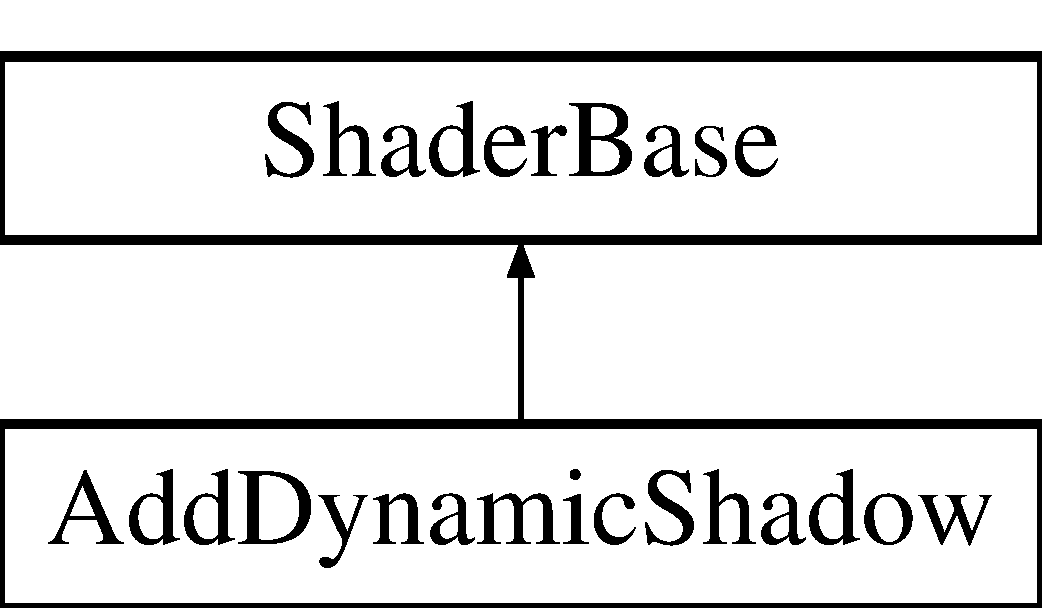
\includegraphics[height=2.000000cm]{classAddDynamicShadow}
\end{center}
\end{figure}
\subsection*{\-Public \-Member \-Functions}
\begin{DoxyCompactItemize}
\item 
\hypertarget{classAddDynamicShadow_a6fbbaa0fff511fbda7fce23a497a2a45}{void {\bfseries \-Init} (void)}\label{classAddDynamicShadow_a6fbbaa0fff511fbda7fce23a497a2a45}

\item 
\hypertarget{classAddDynamicShadow_af4a820a8e394e08d91d020f0b569957f}{void {\bfseries \-Draw} (const glm\-::mat4 \&)}\label{classAddDynamicShadow_af4a820a8e394e08d91d020f0b569957f}

\end{DoxyCompactItemize}


\-The documentation for this class was generated from the following files\-:\begin{DoxyCompactItemize}
\item 
shaders/adddynamicshadow.\-h\item 
shaders/adddynamicshadow.\-cpp\end{DoxyCompactItemize}

\hypertarget{classAddLocalFog}{\section{\-Add\-Local\-Fog \-Class \-Reference}
\label{classAddLocalFog}\index{\-Add\-Local\-Fog@{\-Add\-Local\-Fog}}
}
\-Inheritance diagram for \-Add\-Local\-Fog\-:\begin{figure}[H]
\begin{center}
\leavevmode
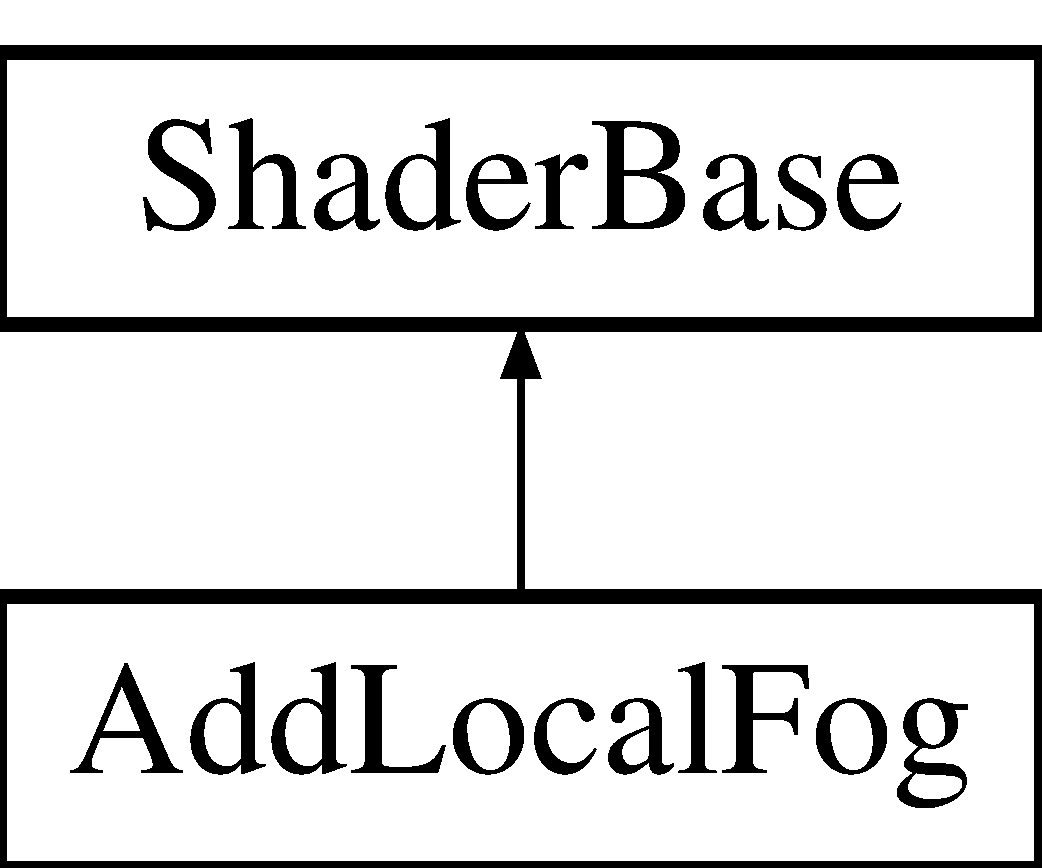
\includegraphics[height=2.000000cm]{classAddLocalFog}
\end{center}
\end{figure}
\subsection*{\-Public \-Member \-Functions}
\begin{DoxyCompactItemize}
\item 
\hypertarget{classAddLocalFog_a4bbf62a52b77842e3855e05b22e1206e}{void {\bfseries \-Init} ()}\label{classAddLocalFog_a4bbf62a52b77842e3855e05b22e1206e}

\item 
\hypertarget{classAddLocalFog_a0aacc047e5f7e74161b7a603dac0a823}{void {\bfseries \-Draw} (const glm\-::vec4 \&point, float ambient)}\label{classAddLocalFog_a0aacc047e5f7e74161b7a603dac0a823}

\end{DoxyCompactItemize}


\-The documentation for this class was generated from the following files\-:\begin{DoxyCompactItemize}
\item 
shaders/addlocalfog.\-h\item 
shaders/addlocalfog.\-cpp\end{DoxyCompactItemize}

\hypertarget{classAddPointLight}{\section{\-Add\-Point\-Light \-Class \-Reference}
\label{classAddPointLight}\index{\-Add\-Point\-Light@{\-Add\-Point\-Light}}
}
\-Inheritance diagram for \-Add\-Point\-Light\-:\begin{figure}[H]
\begin{center}
\leavevmode
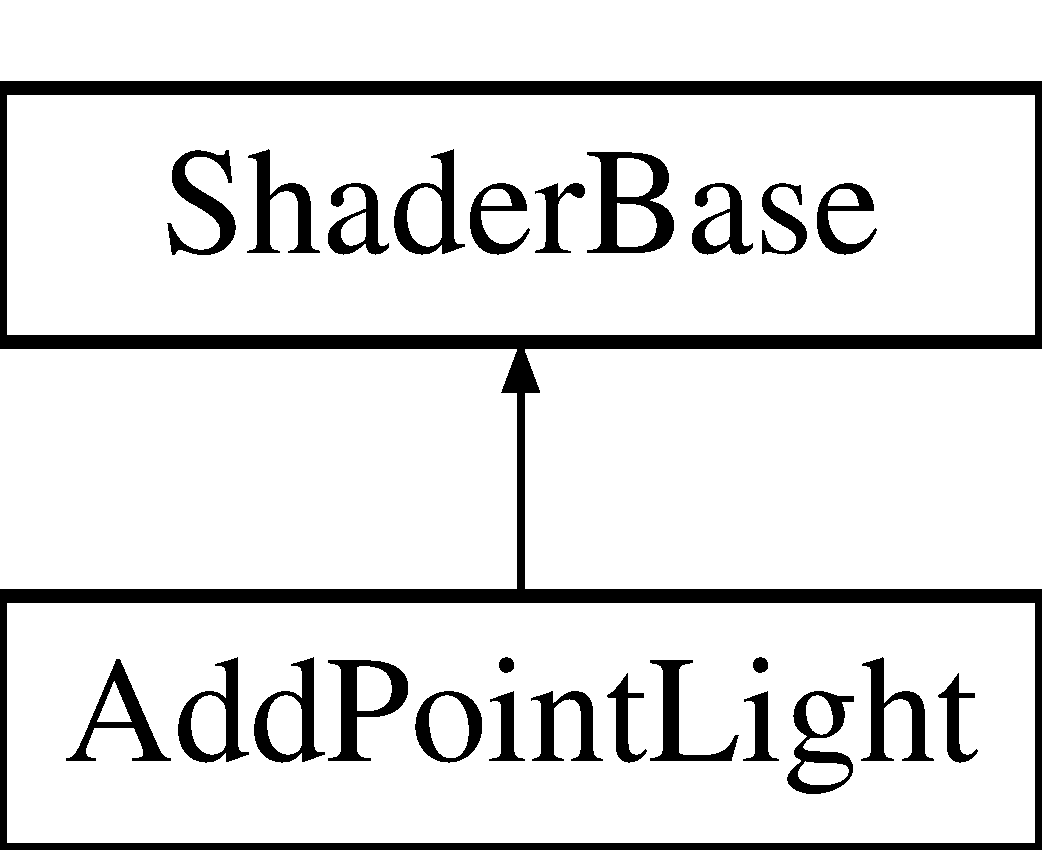
\includegraphics[height=2.000000cm]{classAddPointLight}
\end{center}
\end{figure}
\subsection*{\-Public \-Member \-Functions}
\begin{DoxyCompactItemize}
\item 
\hypertarget{classAddPointLight_a03408127e6be4a0005c364a6c6dc5ca0}{void {\bfseries \-Init} ()}\label{classAddPointLight_a03408127e6be4a0005c364a6c6dc5ca0}

\item 
\hypertarget{classAddPointLight_a816fb5f9e5a595c164f85a0d4b32ce5e}{void {\bfseries \-Draw} (const glm\-::vec3 \&pos, float strength)}\label{classAddPointLight_a816fb5f9e5a595c164f85a0d4b32ce5e}

\end{DoxyCompactItemize}


\-The documentation for this class was generated from the following files\-:\begin{DoxyCompactItemize}
\item 
shaders/addpointlight.\-h\item 
shaders/addpointlight.\-cpp\end{DoxyCompactItemize}

\hypertarget{classAddPointShadow}{\section{\-Add\-Point\-Shadow \-Class \-Reference}
\label{classAddPointShadow}\index{\-Add\-Point\-Shadow@{\-Add\-Point\-Shadow}}
}
\-Inheritance diagram for \-Add\-Point\-Shadow\-:\begin{figure}[H]
\begin{center}
\leavevmode
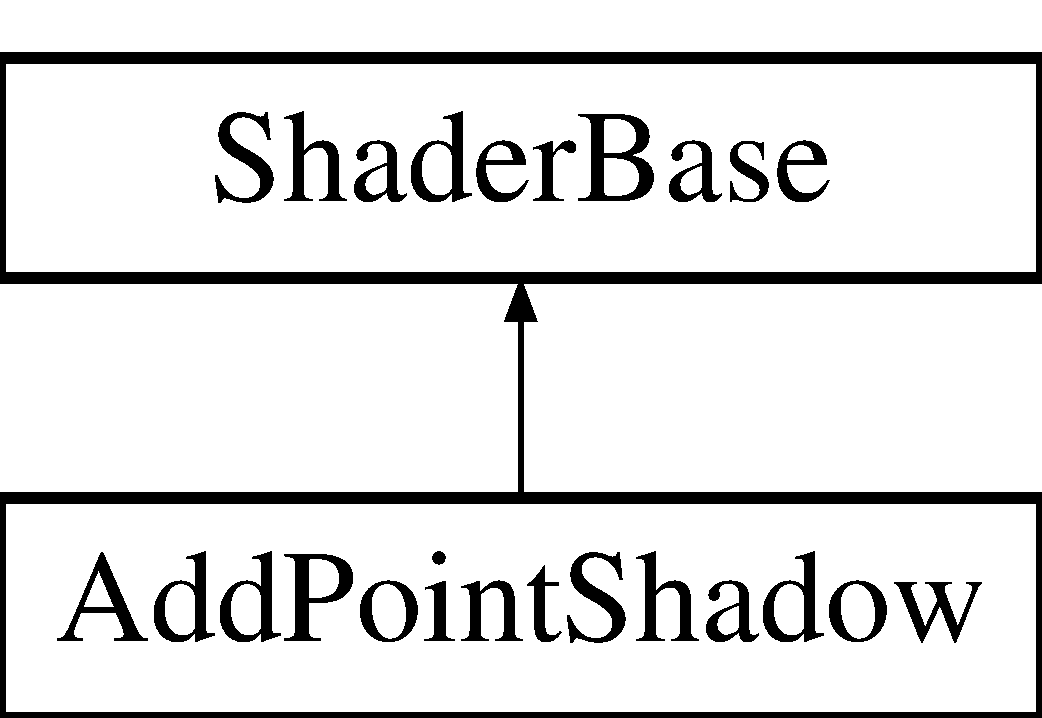
\includegraphics[height=2.000000cm]{classAddPointShadow}
\end{center}
\end{figure}
\subsection*{\-Public \-Member \-Functions}
\begin{DoxyCompactItemize}
\item 
\hypertarget{classAddPointShadow_afbd1b6065f6cd126fa51e9911f14af24}{void {\bfseries \-Init} ()}\label{classAddPointShadow_afbd1b6065f6cd126fa51e9911f14af24}

\item 
\hypertarget{classAddPointShadow_ac087b8fa390d3c92f55cdee5f86d5de0}{void {\bfseries \-Draw} (const glm\-::vec4 \&point, bool for\-Selection=false)}\label{classAddPointShadow_ac087b8fa390d3c92f55cdee5f86d5de0}

\end{DoxyCompactItemize}


\-The documentation for this class was generated from the following files\-:\begin{DoxyCompactItemize}
\item 
shaders/addpointshadow.\-h\item 
shaders/addpointshadow.\-cpp\end{DoxyCompactItemize}

\hypertarget{classAddSSAO}{\section{\-Add\-S\-S\-A\-O \-Class \-Reference}
\label{classAddSSAO}\index{\-Add\-S\-S\-A\-O@{\-Add\-S\-S\-A\-O}}
}
\-Inheritance diagram for \-Add\-S\-S\-A\-O\-:\begin{figure}[H]
\begin{center}
\leavevmode
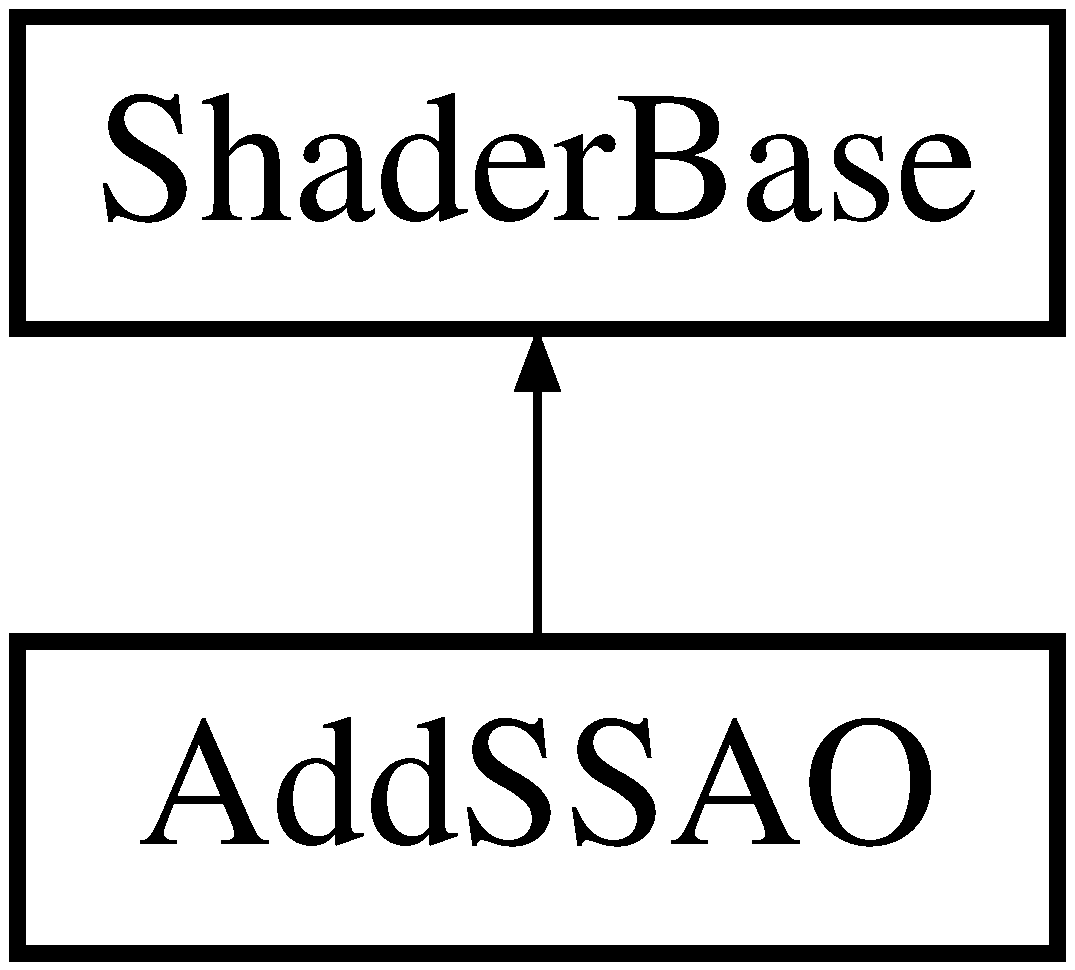
\includegraphics[height=2.000000cm]{classAddSSAO}
\end{center}
\end{figure}
\subsection*{\-Public \-Member \-Functions}
\begin{DoxyCompactItemize}
\item 
\hypertarget{classAddSSAO_a43ef5bf5dc19032e28fc0f45243a39f2}{void {\bfseries \-Init} (void)}\label{classAddSSAO_a43ef5bf5dc19032e28fc0f45243a39f2}

\item 
\hypertarget{classAddSSAO_a99b63b310cdde0d19459b660dcd4c8f9}{void {\bfseries \-Draw} ()}\label{classAddSSAO_a99b63b310cdde0d19459b660dcd4c8f9}

\end{DoxyCompactItemize}


\-The documentation for this class was generated from the following files\-:\begin{DoxyCompactItemize}
\item 
shaders/addssao.\-h\item 
shaders/addssao.\-cpp\end{DoxyCompactItemize}

\hypertarget{structBlenderModel_1_1Animation}{\section{\-Blender\-Model\-:\-:\-Animation \-Struct \-Reference}
\label{structBlenderModel_1_1Animation}\index{\-Blender\-Model\-::\-Animation@{\-Blender\-Model\-::\-Animation}}
}
\subsection*{\-Public \-Attributes}
\begin{DoxyCompactItemize}
\item 
\hypertarget{structBlenderModel_1_1Animation_a438c0737beda1ee6ad8254352a6bcae0}{std\-::string {\bfseries name}}\label{structBlenderModel_1_1Animation_a438c0737beda1ee6ad8254352a6bcae0}

\item 
\hypertarget{structBlenderModel_1_1Animation_a73cdeb48bcc01860a236310bd6d4a670}{std\-::unique\-\_\-ptr$<$ \hyperlink{structAnimationBone}{\-Animation\-Bone}\mbox{[}$\,$\mbox{]}$>$ {\bfseries bones}}\label{structBlenderModel_1_1Animation_a73cdeb48bcc01860a236310bd6d4a670}

\item 
\hypertarget{structBlenderModel_1_1Animation_a8bf004aa13256efce3305a819ce58aa5}{std\-::unique\-\_\-ptr$<$ double\mbox{[}$\,$\mbox{]}$>$ {\bfseries times}}\label{structBlenderModel_1_1Animation_a8bf004aa13256efce3305a819ce58aa5}

\item 
\hypertarget{structBlenderModel_1_1Animation_a641051e7db12e7fb9638b2b29c866fc9}{int {\bfseries num\-Keys}}\label{structBlenderModel_1_1Animation_a641051e7db12e7fb9638b2b29c866fc9}

\item 
\hypertarget{structBlenderModel_1_1Animation_a077c66aa636ca8d3771f6d5b25614c93}{double {\bfseries keys\-Per\-Second}}\label{structBlenderModel_1_1Animation_a077c66aa636ca8d3771f6d5b25614c93}

\item 
\hypertarget{structBlenderModel_1_1Animation_a2ec056e0c909418372ae95e32c1c2efc}{double {\bfseries duration}}\label{structBlenderModel_1_1Animation_a2ec056e0c909418372ae95e32c1c2efc}

\end{DoxyCompactItemize}


\-The documentation for this struct was generated from the following file\-:\begin{DoxyCompactItemize}
\item 
\-Blender\-Model.\-cpp\end{DoxyCompactItemize}

\hypertarget{structAnimationBone}{\section{\-Animation\-Bone \-Struct \-Reference}
\label{structAnimationBone}\index{\-Animation\-Bone@{\-Animation\-Bone}}
}
\subsection*{\-Public \-Attributes}
\begin{DoxyCompactItemize}
\item 
\hypertarget{structAnimationBone_aa6a6274317e040d088d0ef62c4b59113}{std\-::unique\-\_\-ptr$<$ glm\-::mat4\mbox{[}$\,$\mbox{]}$>$ {\bfseries frame\-Matrix}}\label{structAnimationBone_aa6a6274317e040d088d0ef62c4b59113}

\end{DoxyCompactItemize}


\-The documentation for this struct was generated from the following file\-:\begin{DoxyCompactItemize}
\item 
\-Blender\-Model.\-cpp\end{DoxyCompactItemize}

\hypertarget{classAnimationModels}{\section{\-Animation\-Models \-Class \-Reference}
\label{classAnimationModels}\index{\-Animation\-Models@{\-Animation\-Models}}
}
\subsection*{\-Classes}
\begin{DoxyCompactItemize}
\item 
struct {\bfseries \-Data}
\end{DoxyCompactItemize}
\subsection*{\-Public \-Types}
\begin{DoxyCompactItemize}
\item 
enum {\bfseries \-Animation\-Model\-Id} \{ {\bfseries \-Frog}, 
{\bfseries \-Morran}, 
{\bfseries \-Alien}, 
{\bfseries \-L\-A\-S\-T}
 \}
\end{DoxyCompactItemize}
\subsection*{\-Public \-Member \-Functions}
\begin{DoxyCompactItemize}
\item 
\hypertarget{classAnimationModels_a6389af3ee99876374e7a7608b9f2babf}{void {\bfseries \-Init} (void)}\label{classAnimationModels_a6389af3ee99876374e7a7608b9f2babf}

\item 
\hypertarget{classAnimationModels_a66f91816b56d6198aa363896b84806fa}{void {\bfseries \-Draw} (\-Animation\-Model\-Id id, const glm\-::mat4 \&model\-Matrix, double animation\-Start, bool dead) const }\label{classAnimationModels_a66f91816b56d6198aa363896b84806fa}

\end{DoxyCompactItemize}


\-The documentation for this class was generated from the following files\-:\begin{DoxyCompactItemize}
\item 
animationmodels.\-h\item 
animationmodels.\-cpp\end{DoxyCompactItemize}

\hypertarget{classAnimationShader}{\section{\-Animation\-Shader \-Class \-Reference}
\label{classAnimationShader}\index{\-Animation\-Shader@{\-Animation\-Shader}}
}
\-Inheritance diagram for \-Animation\-Shader\-:\begin{figure}[H]
\begin{center}
\leavevmode
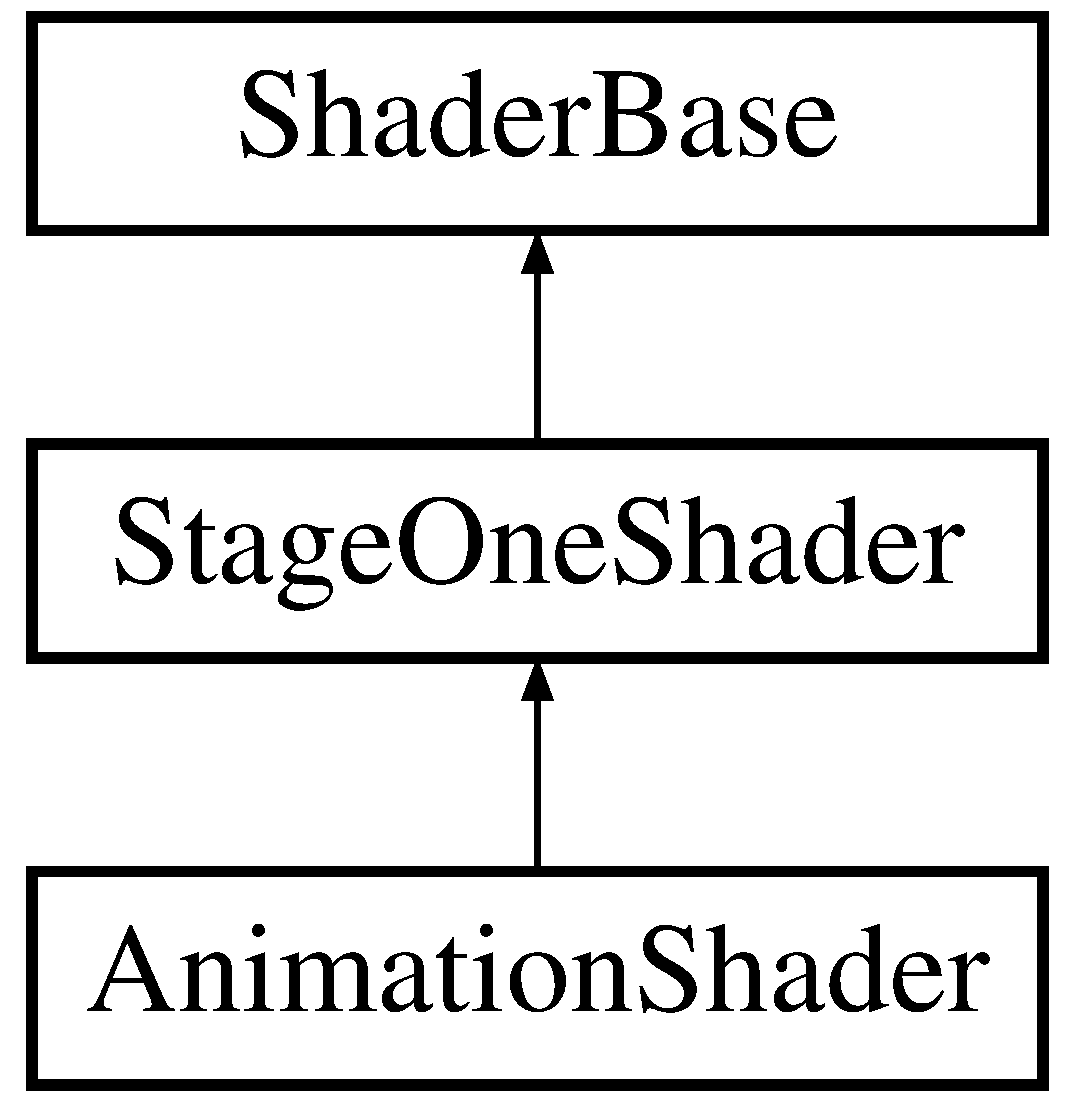
\includegraphics[height=3.000000cm]{classAnimationShader}
\end{center}
\end{figure}
\subsection*{\-Public \-Member \-Functions}
\begin{DoxyCompactItemize}
\item 
\hypertarget{classAnimationShader_a85dd995b06f01e670aee22620c3a9b08}{void {\bfseries \-Model} (const glm\-::mat4 \&)}\label{classAnimationShader_a85dd995b06f01e670aee22620c3a9b08}

\item 
\hypertarget{classAnimationShader_a59a7f87f0053b089061c0bed48e345c7}{void {\bfseries \-First\-Texture} (int ind)}\label{classAnimationShader_a59a7f87f0053b089061c0bed48e345c7}

\item 
\hypertarget{classAnimationShader_a55d021f0f433d680aede9f99eacfa115}{void {\bfseries \-Bones} (const glm\-::mat4 $\ast$, int num)}\label{classAnimationShader_a55d021f0f433d680aede9f99eacfa115}

\item 
\hypertarget{classAnimationShader_af1f2572a6bec7e5661b6e06d18f0fd1f}{void {\bfseries \-Shadowmap} (bool, const glm\-::mat4 \&projectionview)}\label{classAnimationShader_af1f2572a6bec7e5661b6e06d18f0fd1f}

\end{DoxyCompactItemize}
\subsection*{\-Static \-Public \-Member \-Functions}
\begin{DoxyCompactItemize}
\item 
\hypertarget{classAnimationShader_a16df5c606b4cbad58d1bfbbc9a2d8a31}{static \hyperlink{classAnimationShader}{\-Animation\-Shader} $\ast$ {\bfseries \-Make} (void)}\label{classAnimationShader_a16df5c606b4cbad58d1bfbbc9a2d8a31}

\end{DoxyCompactItemize}
\subsection*{\-Protected \-Member \-Functions}
\begin{DoxyCompactItemize}
\item 
\hypertarget{classAnimationShader_aa874fdcfad0626c5ba8a0058ceb59f2c}{virtual void {\bfseries \-Pre\-Link\-Callback} (\-G\-Luint prg)}\label{classAnimationShader_aa874fdcfad0626c5ba8a0058ceb59f2c}

\end{DoxyCompactItemize}


\-The documentation for this class was generated from the following files\-:\begin{DoxyCompactItemize}
\item 
shaders/\-Animation\-Shader.\-h\item 
shaders/\-Animation\-Shader.\-cpp\end{DoxyCompactItemize}

\hypertarget{classBillboard}{\section{\-Billboard \-Class \-Reference}
\label{classBillboard}\index{\-Billboard@{\-Billboard}}
}
\subsection*{\-Public \-Types}
\begin{DoxyCompactItemize}
\item 
enum {\bfseries \-Predefined} \{ \*
{\bfseries tree1}, 
{\bfseries tree1\-Shadow}, 
{\bfseries tree2}, 
{\bfseries tree2\-Shadow}, 
\*
{\bfseries tree3}, 
{\bfseries tree3\-Shadow}, 
{\bfseries num\-Elements}
 \}
\end{DoxyCompactItemize}
\subsection*{\-Public \-Member \-Functions}
\begin{DoxyCompactItemize}
\item 
\hypertarget{classBillboard_a686db9e640bb05fea7870b5ac1d58ffd}{{\bfseries \-Billboard} (int pixel\-Width, int num\-Pictures)}\label{classBillboard_a686db9e640bb05fea7870b5ac1d58ffd}

\item 
\hypertarget{classBillboard_a255cb4eca326ca09b3159f34498c9ac4}{void {\bfseries \-Init} (void)}\label{classBillboard_a255cb4eca326ca09b3159f34498c9ac4}

\item 
\hypertarget{classBillboard_adbe4018f6ba4d825aca779e92f491a11}{int {\bfseries \-Allocate\-Permanent\-Picture} (void)}\label{classBillboard_adbe4018f6ba4d825aca779e92f491a11}

\item 
\hypertarget{classBillboard_a328e66ea7f8dc681e111756ac64beb22}{void {\bfseries \-Free\-Permanent\-Picture} (int)}\label{classBillboard_a328e66ea7f8dc681e111756ac64beb22}

\item 
\hypertarget{classBillboard_a8b4f58d90b1e4369605a07264a237d13}{void {\bfseries \-Enable\-For\-Drawing} (void)}\label{classBillboard_a8b4f58d90b1e4369605a07264a237d13}

\item 
\hypertarget{classBillboard_aa4978a8447c54f86a5907a1854a6cbf0}{void {\bfseries \-Uppdate\-Billboard} (int picture)}\label{classBillboard_aa4978a8447c54f86a5907a1854a6cbf0}

\item 
\hypertarget{classBillboard_aaaf1384dce2e354aa03275e125860cda}{void {\bfseries \-Bind\-Texture} (void)}\label{classBillboard_aaaf1384dce2e354aa03275e125860cda}

\item 
\hypertarget{classBillboard_a2e1dd4f1832fe6a0be6c6e3eb41d039d}{void {\bfseries \-Initialize\-Textures} (\hyperlink{classStageOneShader}{\-Stage\-One\-Shader} $\ast$)}\label{classBillboard_a2e1dd4f1832fe6a0be6c6e3eb41d039d}

\item 
\hypertarget{classBillboard_afda9fa2e0e2452d630e488128c7b38b1}{void {\bfseries \-Draw} (\hyperlink{classStageOneShader}{\-Stage\-One\-Shader} $\ast$shader, const glm\-::mat4 \&model\-Matrix, enum \-Predefined picture)}\label{classBillboard_afda9fa2e0e2452d630e488128c7b38b1}

\end{DoxyCompactItemize}


\-The documentation for this class was generated from the following files\-:\begin{DoxyCompactItemize}
\item 
billboard.\-h\item 
billboard.\-cpp\end{DoxyCompactItemize}

\hypertarget{classBlenderModel}{\section{\-Blender\-Model \-Class \-Reference}
\label{classBlenderModel}\index{\-Blender\-Model@{\-Blender\-Model}}
}
\subsection*{\-Classes}
\begin{DoxyCompactItemize}
\item 
struct \hyperlink{structBlenderModel_1_1Animation}{\-Animation}
\item 
struct \hyperlink{structBlenderModel_1_1Mesh}{\-Mesh}
\end{DoxyCompactItemize}
\subsection*{\-Public \-Member \-Functions}
\begin{DoxyCompactItemize}
\item 
\hypertarget{classBlenderModel_aa0db3fbe9f08981d68a61063479f9d7d}{void {\bfseries \-Init} (const char $\ast$filename, float x\-Rotate\-Correction, bool normalize)}\label{classBlenderModel_aa0db3fbe9f08981d68a61063479f9d7d}

\item 
\hypertarget{classBlenderModel_abea2e166ff05f9425bc3dffba0073571}{void {\bfseries \-Draw\-Animation} (\hyperlink{classAnimationShader}{\-Animation\-Shader} $\ast$shader, const glm\-::mat4 \&model\-Matrix, double animation\-Start, bool dead, const \-G\-Luint $\ast$textures)}\label{classBlenderModel_abea2e166ff05f9425bc3dffba0073571}

\item 
\hypertarget{classBlenderModel_ae095955865ba418b0493ae61b2e0e289}{void {\bfseries \-Draw\-Static} (void)}\label{classBlenderModel_ae095955865ba418b0493ae61b2e0e289}

\item 
\hypertarget{classBlenderModel_a4f3ea09170d536739f31c9506853ae86}{void {\bfseries \-Align} (glm\-::mat4 \&mat) const }\label{classBlenderModel_a4f3ea09170d536739f31c9506853ae86}

\end{DoxyCompactItemize}
\subsection*{\-Static \-Public \-Member \-Functions}
\begin{DoxyCompactItemize}
\item 
\hypertarget{classBlenderModel_af12b4e4b9ca5847ace10484f11be6201}{static void {\bfseries \-Init\-Models} (void)}\label{classBlenderModel_af12b4e4b9ca5847ace10484f11be6201}

\end{DoxyCompactItemize}


\-The documentation for this class was generated from the following files\-:\begin{DoxyCompactItemize}
\item 
\-Blender\-Model.\-h\item 
\-Blender\-Model.\-cpp\end{DoxyCompactItemize}

\hypertarget{classBuildingBlocks}{\section{\-Building\-Blocks \-Class \-Reference}
\label{classBuildingBlocks}\index{\-Building\-Blocks@{\-Building\-Blocks}}
}
\subsection*{\-Public \-Member \-Functions}
\begin{DoxyCompactItemize}
\item 
\hypertarget{classBuildingBlocks_aa28581a2b7760f7326a45e9281b063a4}{void {\bfseries \-Draw} (glm\-::mat4 \&projection)}\label{classBuildingBlocks_aa28581a2b7760f7326a45e9281b063a4}

\item 
\hypertarget{classBuildingBlocks_a03c7abbb552b6377baa59afb14ea0f9f}{void {\bfseries \-Update\-Selection} (int pos)}\label{classBuildingBlocks_a03c7abbb552b6377baa59afb14ea0f9f}

\item 
\hypertarget{classBuildingBlocks_a6e349af5b6aff954c38c589dacbfbfc1}{int {\bfseries \-Current\-Block\-Type} (void) const }\label{classBuildingBlocks_a6e349af5b6aff954c38c589dacbfbfc1}

\end{DoxyCompactItemize}
\subsection*{\-Static \-Public \-Member \-Functions}
\begin{DoxyCompactItemize}
\item 
\hypertarget{classBuildingBlocks_a14df4c7f3de3628ee79fbec433d534b7}{static \hyperlink{classBuildingBlocks}{\-Building\-Blocks} $\ast$ {\bfseries \-Make} (int num\-To\-Display)}\label{classBuildingBlocks_a14df4c7f3de3628ee79fbec433d534b7}

\end{DoxyCompactItemize}


\-The documentation for this class was generated from the following files\-:\begin{DoxyCompactItemize}
\item 
\-Building\-Blocks.\-h\item 
\-Building\-Blocks.\-cpp\end{DoxyCompactItemize}

\hypertarget{structChunkCache_1_1cachunk}{\section{\-Chunk\-Cache\-:\-:cachunk \-Struct \-Reference}
\label{structChunkCache_1_1cachunk}\index{\-Chunk\-Cache\-::cachunk@{\-Chunk\-Cache\-::cachunk}}
}
\subsection*{\-Public \-Attributes}
\begin{DoxyCompactItemize}
\item 
\hypertarget{structChunkCache_1_1cachunk_a0bf5b082f1a23a305a7f9d8c0fbab7c1}{\hyperlink{structChunkCoord}{\-Chunk\-Coord} {\bfseries cc}}\label{structChunkCache_1_1cachunk_a0bf5b082f1a23a305a7f9d8c0fbab7c1}

\item 
\hypertarget{structChunkCache_1_1cachunk_a16f6431cffb6ad986370dc3b19195b62}{unsigned long {\bfseries flag}}\label{structChunkCache_1_1cachunk_a16f6431cffb6ad986370dc3b19195b62}

\item 
\hypertarget{structChunkCache_1_1cachunk_a99831672a39aa2745f333fea0b5f5927}{unsigned int {\bfseries f\-Check\-Sum}}\label{structChunkCache_1_1cachunk_a99831672a39aa2745f333fea0b5f5927}

\item 
\hypertarget{structChunkCache_1_1cachunk_acae83eb407e943b1a0f019e109d670a3}{unsigned long {\bfseries f\-Owner}}\label{structChunkCache_1_1cachunk_acae83eb407e943b1a0f019e109d670a3}

\item 
\hypertarget{structChunkCache_1_1cachunk_a7cc192461695cba3677b5de02668ee50}{unsigned char $\ast$ {\bfseries compressed\-Chunk}}\label{structChunkCache_1_1cachunk_a7cc192461695cba3677b5de02668ee50}

\item 
\hypertarget{structChunkCache_1_1cachunk_a8f56a4411e1b9c6966d4288d3595a153}{int {\bfseries compress\-Size}}\label{structChunkCache_1_1cachunk_a8f56a4411e1b9c6966d4288d3595a153}

\end{DoxyCompactItemize}


\-The documentation for this struct was generated from the following file\-:\begin{DoxyCompactItemize}
\item 
chunkcache.\-h\end{DoxyCompactItemize}

\hypertarget{structchunk}{\section{chunk \-Struct \-Reference}
\label{structchunk}\index{chunk@{chunk}}
}
\subsection*{\-Public \-Member \-Functions}
\begin{DoxyCompactItemize}
\item 
\hypertarget{structchunk_aa7d70d12dfd888f887376ab8dd516b4a}{void {\bfseries \-Uncompress} ()}\label{structchunk_aa7d70d12dfd888f887376ab8dd516b4a}

\item 
\hypertarget{structchunk_a2fd060379e1b7ed20a89660d8fff6c48}{unsigned char {\bfseries \-Get\-Block} (int x, int y, int z) const }\label{structchunk_a2fd060379e1b7ed20a89660d8fff6c48}

\item 
\hypertarget{structchunk_ae1746d5e4644e9cf802ded9556b13d79}{void {\bfseries \-Update\-Neighbor\-Chunks} (void)}\label{structchunk_ae1746d5e4644e9cf802ded9556b13d79}

\item 
\hypertarget{structchunk_ad7cae7413346d48d9efafce21413db46}{void {\bfseries \-Update\-Graphics} (void)}\label{structchunk_ad7cae7413346d48d9efafce21413db46}

\item 
\hypertarget{structchunk_a7595dfb7789020670f912e5471806f05}{void {\bfseries \-Draw} (\hyperlink{classStageOneShader}{\-Stage\-One\-Shader} $\ast$shader, \hyperlink{classChunkShaderPicking}{\-Chunk\-Shader\-Picking} $\ast$pick\-Shader, \-D\-L\-\_\-\-Type dl\-Type)}\label{structchunk_a7595dfb7789020670f912e5471806f05}

\item 
\hypertarget{structchunk_a0ee86d88bb46da9128c598c5288a79c1}{void {\bfseries \-Draw\-Bounding\-Box} (\hyperlink{classStageOneShader}{\-Stage\-One\-Shader} $\ast$shader, int dx, int dy, int dz)}\label{structchunk_a0ee86d88bb46da9128c598c5288a79c1}

\item 
\hypertarget{structchunk_a8da673d2d9e4e59d254c41a83c990bec}{void {\bfseries \-Draw\-Objects} (\hyperlink{classStageOneShader}{\-Stage\-One\-Shader} $\ast$shader, int dx, int dy, int dz, bool for\-Shadows)}\label{structchunk_a8da673d2d9e4e59d254c41a83c990bec}

\item 
\hypertarget{structchunk_a766f32b9d39ba88c213dc0e9f7ddf41d}{void {\bfseries \-Prepare\-Open\-G\-L} (\hyperlink{classStageOneShader}{\-Stage\-One\-Shader} $\ast$shader, \hyperlink{classChunkShaderPicking}{\-Chunk\-Shader\-Picking} $\ast$pick\-Shader, \-D\-L\-\_\-\-Type dl\-Type)}\label{structchunk_a766f32b9d39ba88c213dc0e9f7ddf41d}

\item 
\hypertarget{structchunk_a9a3ec4f479c2408fd267180bc6b49121}{void {\bfseries \-Release\-Open\-G\-L\-Buffers} (void)}\label{structchunk_a9a3ec4f479c2408fd267180bc6b49121}

\item 
\hypertarget{structchunk_a91df6c54dd57941c5cbeef65c399679a}{void {\bfseries \-Set\-Dirty} (bool flag)}\label{structchunk_a91df6c54dd57941c5cbeef65c399679a}

\item 
\hypertarget{structchunk_acb791009026349f4ad4e0935f1a8d71b}{bool {\bfseries \-Is\-Dirty} (void) const }\label{structchunk_acb791009026349f4ad4e0935f1a8d71b}

\item 
\hypertarget{structchunk_adfda9e9e70778685008b19d4a373f721}{void {\bfseries \-Push\-Triangles} (shared\-\_\-ptr$<$ const \hyperlink{classChunkObject}{\-Chunk\-Object} $>$)}\label{structchunk_adfda9e9e70778685008b19d4a373f721}

\item 
\hypertarget{structchunk_ad792a054666a8da861e980ce0d6ece95}{void {\bfseries \-Pop\-Triangles} (void)}\label{structchunk_ad792a054666a8da861e980ce0d6ece95}

\item 
\hypertarget{structchunk_a24e1ec6f965b0f404bbb7525a4887502}{bool {\bfseries \-In\-Sun\-Light} (int ox, int oy, int oz) const }\label{structchunk_a24e1ec6f965b0f404bbb7525a4887502}

\item 
\hypertarget{structchunk_af1b94b9b6a7dbd0c91da5ac5b5c351e3}{float {\bfseries \-Compute\-Ambient\-Light} (int ox, int oy, int oz) const }\label{structchunk_af1b94b9b6a7dbd0c91da5ac5b5c351e3}

\end{DoxyCompactItemize}
\subsection*{\-Static \-Public \-Member \-Functions}
\begin{DoxyCompactItemize}
\item 
\hypertarget{structchunk_a93048b4b978fc47e6acdf0d282079b54}{static unsigned char {\bfseries \-Get\-Chunk\-And\-Block} (signed long long x, signed long long y, signed long long z)}\label{structchunk_a93048b4b978fc47e6acdf0d282079b54}

\item 
\hypertarget{structchunk_ad9de52aea314015991ef7eb30a572411}{static void {\bfseries \-Degrade\-Busy\-List\-\_\-gl} (void)}\label{structchunk_ad9de52aea314015991ef7eb30a572411}

\item 
\hypertarget{structchunk_a3f14f4b5cfa34a8be715aa5b3a44cee0}{static void {\bfseries \-Make\-All\-Chunks\-Dirty} (void)}\label{structchunk_a3f14f4b5cfa34a8be715aa5b3a44cee0}

\end{DoxyCompactItemize}
\subsection*{\-Public \-Attributes}
\begin{DoxyCompactItemize}
\item 
\hypertarget{structchunk_a068473314f595f8880f77b26a85e4543}{\hyperlink{structChunkCoord}{\-Chunk\-Coord} {\bfseries cc}}\label{structchunk_a068473314f595f8880f77b26a85e4543}

\item 
\hypertarget{structchunk_a2f3d6db89375f2c2247d34e999aaeb88}{bool {\bfseries f\-Scheduled\-For\-Computation}}\label{structchunk_a2f3d6db89375f2c2247d34e999aaeb88}

\item 
\hypertarget{structchunk_a9e196a8124a44f42d5499d04c1e3ac5b}{bool {\bfseries f\-Scheduled\-For\-Loading}}\label{structchunk_a9e196a8124a44f42d5499d04c1e3ac5b}

\item 
\hypertarget{structchunk_acea161822a608ba9e4cee340e50478d8}{shared\-\_\-ptr$<$ const \hyperlink{classChunkObject}{\-Chunk\-Object} $>$ {\bfseries f\-Chunk\-Object}}\label{structchunk_acea161822a608ba9e4cee340e50478d8}

\item 
\hypertarget{structchunk_aaf36406c10070a5fdc5508a100f6d3a7}{shared\-\_\-ptr$<$ \hyperlink{structChunkBlocks}{\-Chunk\-Blocks} $>$ {\bfseries f\-Chunk\-Blocks}}\label{structchunk_aaf36406c10070a5fdc5508a100f6d3a7}

\item 
\hypertarget{structchunk_a27a8b1efa7f3ddc6f1df8c2a789bc109}{\-G\-Luint {\bfseries f\-Buffer\-Id} \mbox{[}256\mbox{]}}\label{structchunk_a27a8b1efa7f3ddc6f1df8c2a789bc109}

\item 
\hypertarget{structchunk_adfc36fb66a3442bf328f9d1bb94d19c3}{\-G\-Luint {\bfseries f\-Vao} \mbox{[}256\mbox{]}}\label{structchunk_adfc36fb66a3442bf328f9d1bb94d19c3}

\item 
\hypertarget{structchunk_ac254adeb6ad5c60c740d2aa30bbc76fd}{bool {\bfseries f\-Buffers\-Defined}}\label{structchunk_ac254adeb6ad5c60c740d2aa30bbc76fd}

\end{DoxyCompactItemize}


\-The documentation for this struct was generated from the following files\-:\begin{DoxyCompactItemize}
\item 
chunk.\-h\item 
chunk.\-cpp\end{DoxyCompactItemize}

\hypertarget{structChunkBlocks}{\section{\-Chunk\-Blocks \-Struct \-Reference}
\label{structChunkBlocks}\index{\-Chunk\-Blocks@{\-Chunk\-Blocks}}
}
\subsection*{\-Classes}
\begin{DoxyCompactItemize}
\item 
struct \hyperlink{structChunkBlocks_1_1JellyBlock}{\-Jelly\-Block}
\end{DoxyCompactItemize}
\subsection*{\-Public \-Member \-Functions}
\begin{DoxyCompactItemize}
\item 
\hypertarget{structChunkBlocks_aa1c7b35454e63e1fe2e4d36f3bc8b43b}{void {\bfseries \-Uncompress} (void)}\label{structChunkBlocks_aa1c7b35454e63e1fe2e4d36f3bc8b43b}

\item 
\hypertarget{structChunkBlocks_a368d3c0aa49ddbca5f049280f36c1436}{void {\bfseries \-Add\-Timer\-Jelly\-Block} (unsigned char dx, unsigned char dy, unsigned char dz, double delta\-Time)}\label{structChunkBlocks_a368d3c0aa49ddbca5f049280f36c1436}

\item 
\hypertarget{structChunkBlocks_a7a89d2f96506d7239a3f40c43fe5221e}{void {\bfseries \-Test\-Jelly\-Block\-Timeout} (bool unconditionally=false)}\label{structChunkBlocks_a7a89d2f96506d7239a3f40c43fe5221e}

\item 
\hypertarget{structChunkBlocks_af1e1e0891ad48b303439103dd2cec9f4}{void {\bfseries \-Command\-Block\-Update} (const \hyperlink{structChunkCoord}{\-Chunk\-Coord} \&cc, int dx, int dy, int dz, int type)}\label{structChunkBlocks_af1e1e0891ad48b303439103dd2cec9f4}

\item 
\hypertarget{structChunkBlocks_acf35144625684f0cdaef487a4fbab29c}{void {\bfseries \-Set\-Teleport} (int x, int y, int z)}\label{structChunkBlocks_acf35144625684f0cdaef487a4fbab29c}

\item 
\hypertarget{structChunkBlocks_a71df5c97bb349fe1a730592c8aeabb76}{bool {\bfseries block\-Is\-Compl\-Transp} (unsigned char bl) const }\label{structChunkBlocks_a71df5c97bb349fe1a730592c8aeabb76}

\end{DoxyCompactItemize}
\subsection*{\-Static \-Public \-Member \-Functions}
\begin{DoxyCompactItemize}
\item 
\hypertarget{structChunkBlocks_ad7f0d73cb7a7ac9b9a0e9adbd78b1895}{static void {\bfseries \-Init\-Static} (void)}\label{structChunkBlocks_ad7f0d73cb7a7ac9b9a0e9adbd78b1895}

\item 
\hypertarget{structChunkBlocks_a15714b8cfd908d16ae64d2207d3abe75}{static bool {\bfseries block\-Is\-Semi\-Transp} (unsigned char bl)}\label{structChunkBlocks_a15714b8cfd908d16ae64d2207d3abe75}

\item 
\hypertarget{structChunkBlocks_a573e6f9e5c01366283ea2dbe4ce43914}{static bool {\bfseries rigid} (unsigned char bl)}\label{structChunkBlocks_a573e6f9e5c01366283ea2dbe4ce43914}

\item 
\hypertarget{structChunkBlocks_a33b837566d8159b2141e0310e15024a9}{static bool {\bfseries plastic} (unsigned char bl)}\label{structChunkBlocks_a33b837566d8159b2141e0310e15024a9}

\end{DoxyCompactItemize}
\subsection*{\-Public \-Attributes}
\begin{DoxyCompactItemize}
\item 
\hypertarget{structChunkBlocks_ae1f57a236b339a0615ae340a3444659c}{unsigned long {\bfseries flag}}\label{structChunkBlocks_ae1f57a236b339a0615ae340a3444659c}

\item 
\hypertarget{structChunkBlocks_a24f6ef161d980e4451674aa1077b00ca}{unsigned int {\bfseries f\-Checksum}}\label{structChunkBlocks_a24f6ef161d980e4451674aa1077b00ca}

\item 
\hypertarget{structChunkBlocks_a7eb91bd11b29bc7a293ebb34a19b8023}{unsigned long {\bfseries f\-Owner}}\label{structChunkBlocks_a7eb91bd11b29bc7a293ebb34a19b8023}

\item 
\hypertarget{structChunkBlocks_a8e97b341e859cda581caefcf15e03705}{\hyperlink{structchunk}{chunk} $\ast$ {\bfseries f\-Chunk}}\label{structChunkBlocks_a8e97b341e859cda581caefcf15e03705}

\item 
\hypertarget{structChunkBlocks_a29da89a4fba0f0fc56217a6d0944beac}{double {\bfseries f\-Checksum\-Timeout}}\label{structChunkBlocks_a29da89a4fba0f0fc56217a6d0944beac}

\item 
\hypertarget{structChunkBlocks_a16aa1c3dbb8143c7654051ce40bddcdd}{std\-::unique\-\_\-ptr$<$ unsigned char\mbox{[}$\,$\mbox{]}$>$ {\bfseries f\-Compressed\-Chunk}}\label{structChunkBlocks_a16aa1c3dbb8143c7654051ce40bddcdd}

\item 
\hypertarget{structChunkBlocks_ab276a22dfcfe671bf9a0bfcb548fa5fb}{int {\bfseries compress\-Size}}\label{structChunkBlocks_ab276a22dfcfe671bf9a0bfcb548fa5fb}

\item 
\hypertarget{structChunkBlocks_a305279bad2806c9d75a78fa0ae762428}{std\-::unique\-\_\-ptr$<$ unsigned char\mbox{[}$\,$\mbox{]}$>$ {\bfseries f\-Chunk\-Data}}\label{structChunkBlocks_a305279bad2806c9d75a78fa0ae762428}

\item 
\hypertarget{structChunkBlocks_afa1dd96d29ae5f8e587efe93572497f1}{bool {\bfseries f\-Checksum\-Test\-Needed}}\label{structChunkBlocks_afa1dd96d29ae5f8e587efe93572497f1}

\end{DoxyCompactItemize}


\-The documentation for this struct was generated from the following files\-:\begin{DoxyCompactItemize}
\item 
\-Chunk\-Blocks.\-h\item 
\-Chunk\-Blocks.\-cpp\end{DoxyCompactItemize}

\hypertarget{classChunkCache}{\section{\-Chunk\-Cache \-Class \-Reference}
\label{classChunkCache}\index{\-Chunk\-Cache@{\-Chunk\-Cache}}
}
\subsection*{\-Classes}
\begin{DoxyCompactItemize}
\item 
struct \hyperlink{structChunkCache_1_1cachunk}{cachunk}
\end{DoxyCompactItemize}
\subsection*{\-Public \-Member \-Functions}
\begin{DoxyCompactItemize}
\item 
\hypertarget{classChunkCache_a55102f0f514b09b47dae4183157595b1}{void {\bfseries \-Set\-Cache\-Dir} (const char $\ast$)}\label{classChunkCache_a55102f0f514b09b47dae4183157595b1}

\item 
\hypertarget{classChunkCache_a461d4ef9f261f0e6e126d9148bcac50e}{bool {\bfseries \-Is\-Chunk\-In\-Cache} (const \hyperlink{structChunkCoord}{\-Chunk\-Coord} $\ast$cc)}\label{classChunkCache_a461d4ef9f261f0e6e126d9148bcac50e}

\item 
\hypertarget{classChunkCache_ab142e310653e49dfd4b6eec5097d3ced}{void {\bfseries \-Save\-Chunk\-In\-Cache} (const \hyperlink{structChunkCache_1_1cachunk}{cachunk} $\ast$)}\label{classChunkCache_ab142e310653e49dfd4b6eec5097d3ced}

\item 
\hypertarget{classChunkCache_a6f94c1bcea2290cd0f54d4dd5d58d99a}{std\-::shared\-\_\-ptr$<$ \hyperlink{structChunkBlocks}{\-Chunk\-Blocks} $>$ {\bfseries \-Load\-Chunk\-From\-Cache} (const \hyperlink{structChunkCoord}{\-Chunk\-Coord} $\ast$cc)}\label{classChunkCache_a6f94c1bcea2290cd0f54d4dd5d58d99a}

\end{DoxyCompactItemize}
\subsection*{\-Static \-Public \-Attributes}
\begin{DoxyCompactItemize}
\item 
\hypertarget{classChunkCache_a1140dc6c19fab12ef83a7fd2267281f3}{static \hyperlink{classChunkCache}{\-Chunk\-Cache} {\bfseries fg\-Chunk\-Cache}}\label{classChunkCache_a1140dc6c19fab12ef83a7fd2267281f3}

\end{DoxyCompactItemize}


\-The documentation for this class was generated from the following files\-:\begin{DoxyCompactItemize}
\item 
chunkcache.\-h\item 
chunkcache.\-cpp\end{DoxyCompactItemize}

\hypertarget{structChunkCoord}{\section{\-Chunk\-Coord \-Struct \-Reference}
\label{structChunkCoord}\index{\-Chunk\-Coord@{\-Chunk\-Coord}}
}
\subsection*{\-Public \-Member \-Functions}
\begin{DoxyCompactItemize}
\item 
\hypertarget{structChunkCoord_aff7009253580e68330cf95c9467a6c58}{bool {\bfseries operator$<$} (const \hyperlink{structChunkCoord}{\-Chunk\-Coord} \&other) const }\label{structChunkCoord_aff7009253580e68330cf95c9467a6c58}

\end{DoxyCompactItemize}
\subsection*{\-Public \-Attributes}
\begin{DoxyCompactItemize}
\item 
\hypertarget{structChunkCoord_acfafebe94c4a2679f0781e70690e412b}{int {\bfseries x}}\label{structChunkCoord_acfafebe94c4a2679f0781e70690e412b}

\item 
\hypertarget{structChunkCoord_a9b618a411177df2a9e0f2b059184495e}{int {\bfseries y}}\label{structChunkCoord_a9b618a411177df2a9e0f2b059184495e}

\item 
\hypertarget{structChunkCoord_ac4d9ca409f8eee8253a77affba02f630}{int {\bfseries z}}\label{structChunkCoord_ac4d9ca409f8eee8253a77affba02f630}

\end{DoxyCompactItemize}


\-The documentation for this struct was generated from the following file\-:\begin{DoxyCompactItemize}
\item 
chunk.\-h\end{DoxyCompactItemize}

\hypertarget{structChunkDist}{\section{\-Chunk\-Dist \-Struct \-Reference}
\label{structChunkDist}\index{\-Chunk\-Dist@{\-Chunk\-Dist}}
}
\subsection*{\-Public \-Attributes}
\begin{DoxyCompactItemize}
\item 
\hypertarget{structChunkDist_a7deb5c6e44b43c57ec1eb5d72ddcd1d1}{char {\bfseries dx}}\label{structChunkDist_a7deb5c6e44b43c57ec1eb5d72ddcd1d1}

\item 
\hypertarget{structChunkDist_a7ba7baed72b9432e69f7e246ee02dc9a}{char {\bfseries dy}}\label{structChunkDist_a7ba7baed72b9432e69f7e246ee02dc9a}

\item 
\hypertarget{structChunkDist_a3ab9ab3f997301327e33e9f94b830dde}{char {\bfseries dz}}\label{structChunkDist_a3ab9ab3f997301327e33e9f94b830dde}

\item 
\hypertarget{structChunkDist_aa15f7a59481270053d92b8c20e26b2fe}{float {\bfseries distance}}\label{structChunkDist_aa15f7a59481270053d92b8c20e26b2fe}

\end{DoxyCompactItemize}


\-The documentation for this struct was generated from the following file\-:\begin{DoxyCompactItemize}
\item 
render.\-cpp\end{DoxyCompactItemize}

\hypertarget{structSuperChunk_1_1chunkInfo}{\section{\-Super\-Chunk\-:\-:chunk\-Info \-Struct \-Reference}
\label{structSuperChunk_1_1chunkInfo}\index{\-Super\-Chunk\-::chunk\-Info@{\-Super\-Chunk\-::chunk\-Info}}
}
\subsection*{\-Public \-Attributes}
\begin{DoxyCompactItemize}
\item 
\hypertarget{structSuperChunk_1_1chunkInfo_a90490f0fa34bbce9babf6b0ab2ffb491}{unsigned char {\bfseries flag}}\label{structSuperChunk_1_1chunkInfo_a90490f0fa34bbce9babf6b0ab2ffb491}

\item 
\hypertarget{structSuperChunk_1_1chunkInfo_a4e2cc31a2d503cc86a2c4b9a9565e037}{unsigned char {\bfseries x}}\label{structSuperChunk_1_1chunkInfo_a4e2cc31a2d503cc86a2c4b9a9565e037}

\item 
\hypertarget{structSuperChunk_1_1chunkInfo_a80e206ada4eeae53b76445c2ef442365}{unsigned char {\bfseries y}}\label{structSuperChunk_1_1chunkInfo_a80e206ada4eeae53b76445c2ef442365}

\item 
\hypertarget{structSuperChunk_1_1chunkInfo_aa2335fb7450abb91566d7f707e5e4800}{unsigned char {\bfseries z}}\label{structSuperChunk_1_1chunkInfo_aa2335fb7450abb91566d7f707e5e4800}

\end{DoxyCompactItemize}


\-The documentation for this struct was generated from the following file\-:\begin{DoxyCompactItemize}
\item 
\-Super\-Chunk\-Manager.\-h\end{DoxyCompactItemize}

\hypertarget{classChunkObject}{\section{\-Chunk\-Object \-Class \-Reference}
\label{classChunkObject}\index{\-Chunk\-Object@{\-Chunk\-Object}}
}
\subsection*{\-Classes}
\begin{DoxyCompactItemize}
\item 
struct \hyperlink{structChunkObject_1_1SpecialObject}{\-Special\-Object}
\end{DoxyCompactItemize}
\subsection*{\-Public \-Member \-Functions}
\begin{DoxyCompactItemize}
\item 
\hypertarget{classChunkObject_a937c93c788817c34d29b689c79f13a59}{int {\bfseries \-Vertex\-Size} (int bl) const }\label{classChunkObject_a937c93c788817c34d29b689c79f13a59}

\item 
\hypertarget{classChunkObject_afaae23fe47adcde9eca46bc1237d97b7}{bool {\bfseries \-Empty} (void) const }\label{classChunkObject_afaae23fe47adcde9eca46bc1237d97b7}

\item 
\hypertarget{classChunkObject_a5ce77de941e41edae73d6c2fb696ccaf}{void {\bfseries \-Find\-Special\-Objects} (const \hyperlink{structchunk}{chunk} $\ast$cp)}\label{classChunkObject_a5ce77de941e41edae73d6c2fb696ccaf}

\end{DoxyCompactItemize}
\subsection*{\-Static \-Public \-Member \-Functions}
\begin{DoxyCompactItemize}
\item 
\hypertarget{classChunkObject_a6b4f077c0fd2c0f716f63159a187b557}{static unique\-\_\-ptr$<$ \hyperlink{classChunkObject}{\-Chunk\-Object} $>$ {\bfseries \-Make} (const \hyperlink{structchunk}{chunk} $\ast$cp, bool picking\-Mode, int pdx, int pdy, int pdz)}\label{classChunkObject_a6b4f077c0fd2c0f716f63159a187b557}

\end{DoxyCompactItemize}
\subsection*{\-Public \-Attributes}
\begin{DoxyCompactItemize}
\item 
\hypertarget{classChunkObject_a2c0bf18b0723a9e20fe631d7e099e3dd}{std\-::vector$<$ \hyperlink{structTriangleSurfacef}{\-Triangle\-Surfacef} $>$ {\bfseries f\-Visible\-Triangles} \mbox{[}256\mbox{]}}\label{classChunkObject_a2c0bf18b0723a9e20fe631d7e099e3dd}

\item 
\hypertarget{classChunkObject_af351f75b98f8e66865285b0999846f42}{char {\bfseries f\-Bound\-X\-Min}}\label{classChunkObject_af351f75b98f8e66865285b0999846f42}

\item 
\hypertarget{classChunkObject_aeb4a714995d2e47a8b6f956302fbbb04}{char {\bfseries f\-Bound\-X\-Max}}\label{classChunkObject_aeb4a714995d2e47a8b6f956302fbbb04}

\item 
\hypertarget{classChunkObject_adf1f1536c49de477f583b4032419fa3d}{char {\bfseries f\-Bound\-Y\-Min}}\label{classChunkObject_adf1f1536c49de477f583b4032419fa3d}

\item 
\hypertarget{classChunkObject_aa58560b8a005b223a15dfe03799f55c8}{char {\bfseries f\-Bound\-Y\-Max}}\label{classChunkObject_aa58560b8a005b223a15dfe03799f55c8}

\item 
\hypertarget{classChunkObject_ac659b3d9058cda60b9ec2accfac58623}{char {\bfseries f\-Bound\-Z\-Min}}\label{classChunkObject_ac659b3d9058cda60b9ec2accfac58623}

\item 
\hypertarget{classChunkObject_a2716b8931b56f5ef33a27e3250d39cfa}{char {\bfseries f\-Bound\-Z\-Max}}\label{classChunkObject_a2716b8931b56f5ef33a27e3250d39cfa}

\item 
\hypertarget{classChunkObject_a0b8cedbb86c56b0c7cb5033a4336b687}{unique\-\_\-ptr$<$ \hyperlink{structChunkObject_1_1SpecialObject}{\-Special\-Object}\mbox{[}$\,$\mbox{]}$>$ {\bfseries f\-Tree\-List}}\label{classChunkObject_a0b8cedbb86c56b0c7cb5033a4336b687}

\item 
\hypertarget{classChunkObject_a54aaa4d000bafe8d0c71eef55832866e}{int {\bfseries f\-Num\-Tree}}\label{classChunkObject_a54aaa4d000bafe8d0c71eef55832866e}

\item 
\hypertarget{classChunkObject_aae87a2cac0d2d4a4516ea581e140fd1c}{unique\-\_\-ptr$<$ \hyperlink{structChunkObject_1_1SpecialObject}{\-Special\-Object}\mbox{[}$\,$\mbox{]}$>$ {\bfseries f\-Lamp\-List}}\label{classChunkObject_aae87a2cac0d2d4a4516ea581e140fd1c}

\item 
\hypertarget{classChunkObject_a2806cfb86ec247403262314269621c03}{int {\bfseries f\-Num\-Lamps}}\label{classChunkObject_a2806cfb86ec247403262314269621c03}

\item 
\hypertarget{classChunkObject_a990fae3ceabdfe55878ee82286c40d01}{unique\-\_\-ptr$<$ \hyperlink{structChunkObject_1_1SpecialObject}{\-Special\-Object}\mbox{[}$\,$\mbox{]}$>$ {\bfseries f\-Fog\-List}}\label{classChunkObject_a990fae3ceabdfe55878ee82286c40d01}

\item 
\hypertarget{classChunkObject_aac98326a70f3497c4422e9b7b6a918cb}{int {\bfseries f\-Num\-Fogs}}\label{classChunkObject_aac98326a70f3497c4422e9b7b6a918cb}

\item 
\hypertarget{classChunkObject_a6a76f5738ea7909c576655d305dba06d}{unique\-\_\-ptr$<$ \hyperlink{structChunkObject_1_1SpecialObject}{\-Special\-Object}\mbox{[}$\,$\mbox{]}$>$ {\bfseries f\-Treasure\-List}}\label{classChunkObject_a6a76f5738ea7909c576655d305dba06d}

\item 
\hypertarget{classChunkObject_ac2b3122a72b76727bba203df409ded26}{int {\bfseries f\-Num\-Treasures}}\label{classChunkObject_ac2b3122a72b76727bba203df409ded26}

\item 
\hypertarget{classChunkObject_a50b121bbbc1fca55d5f6e26215857106}{\hyperlink{structchunk}{chunk} $\ast$ {\bfseries f\-Chunk}}\label{classChunkObject_a50b121bbbc1fca55d5f6e26215857106}

\end{DoxyCompactItemize}


\-The documentation for this class was generated from the following files\-:\begin{DoxyCompactItemize}
\item 
\-Chunk\-Object.\-h\item 
\-Chunk\-Object.\-cpp\end{DoxyCompactItemize}

\hypertarget{structChunkOffsetCoord}{\section{\-Chunk\-Offset\-Coord \-Struct \-Reference}
\label{structChunkOffsetCoord}\index{\-Chunk\-Offset\-Coord@{\-Chunk\-Offset\-Coord}}
}
\subsection*{\-Public \-Attributes}
\begin{DoxyCompactItemize}
\item 
\hypertarget{structChunkOffsetCoord_a34b2dd60d69723ecffb9485f39376eea}{unsigned short {\bfseries x}}\label{structChunkOffsetCoord_a34b2dd60d69723ecffb9485f39376eea}

\item 
\hypertarget{structChunkOffsetCoord_ae0a82747626ffcacc8df6ef8d3cd90e7}{unsigned short {\bfseries y}}\label{structChunkOffsetCoord_ae0a82747626ffcacc8df6ef8d3cd90e7}

\item 
\hypertarget{structChunkOffsetCoord_a4044761f8368e90e3082fdb9a4e6d03c}{unsigned short {\bfseries z}}\label{structChunkOffsetCoord_a4044761f8368e90e3082fdb9a4e6d03c}

\end{DoxyCompactItemize}


\-The documentation for this struct was generated from the following file\-:\begin{DoxyCompactItemize}
\item 
chunk.\-h\end{DoxyCompactItemize}

\hypertarget{classChunkProcess}{\section{\-Chunk\-Process \-Class \-Reference}
\label{classChunkProcess}\index{\-Chunk\-Process@{\-Chunk\-Process}}
}
\subsection*{\-Public \-Member \-Functions}
\begin{DoxyCompactItemize}
\item 
\hypertarget{classChunkProcess_ad0f2b2ee2eddd45b315997ed40417be9}{void {\bfseries \-Init} (int num\-Threads)}\label{classChunkProcess_ad0f2b2ee2eddd45b315997ed40417be9}

\item 
\hypertarget{classChunkProcess_a64eb2420d93d3c526117f699c7ffc03c}{void {\bfseries \-Add\-Task\-Compute\-Chunk} (\hyperlink{structchunk}{chunk} $\ast$)}\label{classChunkProcess_a64eb2420d93d3c526117f699c7ffc03c}

\item 
\hypertarget{classChunkProcess_aa48298522a70877bea81dae4e9772e27}{void {\bfseries \-Poll} (void)}\label{classChunkProcess_aa48298522a70877bea81dae4e9772e27}

\item 
\hypertarget{classChunkProcess_a2a7c5b8db6530dd24cf5d1c30f8ae2fc}{void {\bfseries \-Add\-Task\-New\-Chunk} (unique\-\_\-ptr$<$ \hyperlink{structChunkBlocks}{\-Chunk\-Blocks} $>$)}\label{classChunkProcess_a2a7c5b8db6530dd24cf5d1c30f8ae2fc}

\item 
\hypertarget{classChunkProcess_ae121487fd3afdc247d71a58c4ef8226e}{void {\bfseries \-Request\-Terminate} (void)}\label{classChunkProcess_ae121487fd3afdc247d71a58c4ef8226e}

\end{DoxyCompactItemize}


\-The documentation for this class was generated from the following files\-:\begin{DoxyCompactItemize}
\item 
\-Chunk\-Process.\-h\item 
\-Chunk\-Process.\-cpp\end{DoxyCompactItemize}

\hypertarget{classChunkShader}{\section{\-Chunk\-Shader \-Class \-Reference}
\label{classChunkShader}\index{\-Chunk\-Shader@{\-Chunk\-Shader}}
}
\-Inheritance diagram for \-Chunk\-Shader\-:\begin{figure}[H]
\begin{center}
\leavevmode
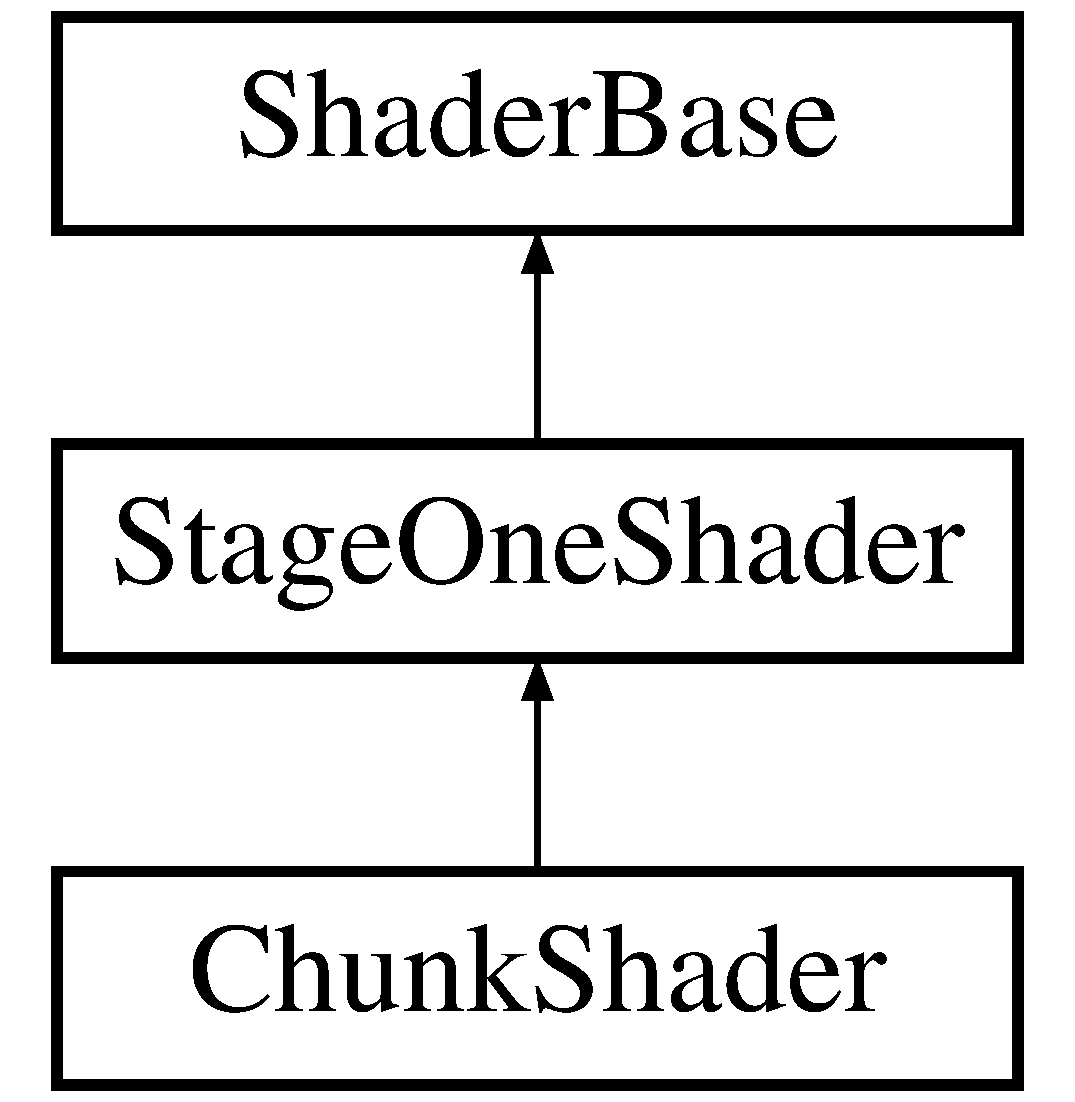
\includegraphics[height=3.000000cm]{classChunkShader}
\end{center}
\end{figure}
\subsection*{\-Public \-Member \-Functions}
\begin{DoxyCompactItemize}
\item 
\hypertarget{classChunkShader_ae69371ea31b05cf34ab85357e2ce7588}{void {\bfseries \-Model} (const glm\-::mat4 \&)}\label{classChunkShader_ae69371ea31b05cf34ab85357e2ce7588}

\item 
\hypertarget{classChunkShader_ae12bf7919d207ec1a9a51103f4e0ca58}{void {\bfseries \-First\-Texture} (int ind)}\label{classChunkShader_ae12bf7919d207ec1a9a51103f4e0ca58}

\item 
\hypertarget{classChunkShader_a62334139662241090f92e742f92c5473}{virtual void {\bfseries \-Texture\-Offset\-Multi} (float offs\-X, float offs\-Y, float mult)}\label{classChunkShader_a62334139662241090f92e742f92c5473}

\end{DoxyCompactItemize}
\subsection*{\-Static \-Public \-Member \-Functions}
\begin{DoxyCompactItemize}
\item 
\hypertarget{classChunkShader_a9bfc76370f471b02c61c9435f7ab969c}{static \hyperlink{classChunkShader}{\-Chunk\-Shader} $\ast$ {\bfseries \-Make} (void)}\label{classChunkShader_a9bfc76370f471b02c61c9435f7ab969c}

\end{DoxyCompactItemize}
\subsection*{\-Protected \-Member \-Functions}
\begin{DoxyCompactItemize}
\item 
\hypertarget{classChunkShader_ae348affb10b3fd69e97d3b64b821d44e}{virtual void {\bfseries \-Pre\-Link\-Callback} (\-G\-Luint prg)}\label{classChunkShader_ae348affb10b3fd69e97d3b64b821d44e}

\end{DoxyCompactItemize}


\-The documentation for this class was generated from the following files\-:\begin{DoxyCompactItemize}
\item 
shaders/\-Chunk\-Shader.\-h\item 
shaders/\-Chunk\-Shader.\-cpp\end{DoxyCompactItemize}

\hypertarget{classChunkShaderPicking}{\section{\-Chunk\-Shader\-Picking \-Class \-Reference}
\label{classChunkShaderPicking}\index{\-Chunk\-Shader\-Picking@{\-Chunk\-Shader\-Picking}}
}
\-Inheritance diagram for \-Chunk\-Shader\-Picking\-:\begin{figure}[H]
\begin{center}
\leavevmode
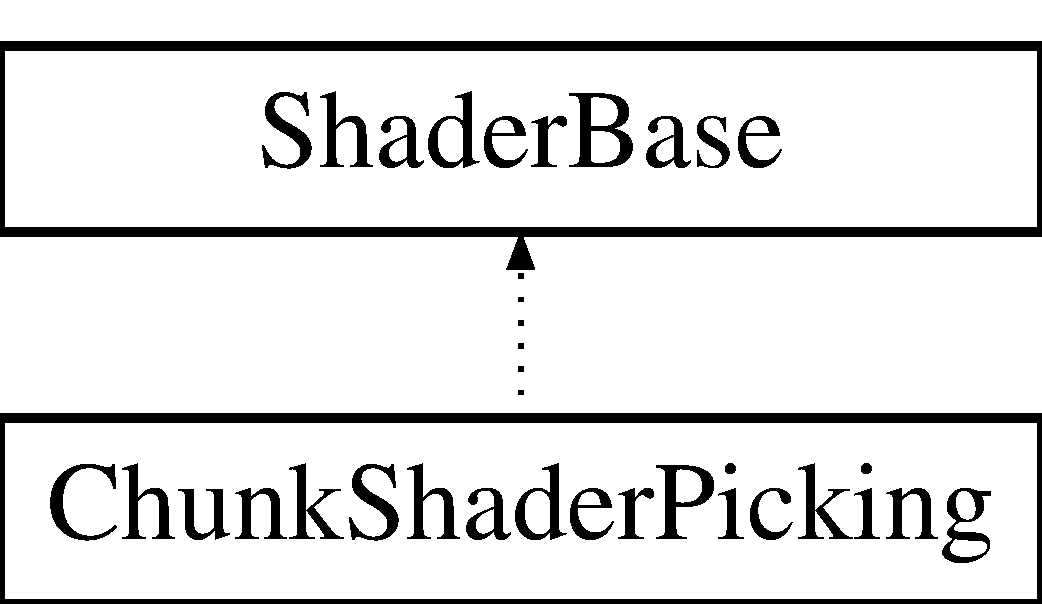
\includegraphics[height=2.000000cm]{classChunkShaderPicking}
\end{center}
\end{figure}
\subsection*{\-Public \-Member \-Functions}
\begin{DoxyCompactItemize}
\item 
\hypertarget{classChunkShaderPicking_a27218004043cc389e40489db791c4f9f}{void {\bfseries \-Enable\-Program} (void)}\label{classChunkShaderPicking_a27218004043cc389e40489db791c4f9f}

\item 
\hypertarget{classChunkShaderPicking_a71e05eac6b9a07f30520a34a8841c0e4}{void {\bfseries \-Disable\-Program} (void)}\label{classChunkShaderPicking_a71e05eac6b9a07f30520a34a8841c0e4}

\item 
\hypertarget{classChunkShaderPicking_ae8115eb6eb1bb3537b743b67d8ca91e9}{void {\bfseries \-Model} (const glm\-::mat4 \&)}\label{classChunkShaderPicking_ae8115eb6eb1bb3537b743b67d8ca91e9}

\item 
\hypertarget{classChunkShaderPicking_a04d783cbb2b3efe1410cbe0e28d9977c}{void {\bfseries \-View} (const glm\-::mat4 \&)}\label{classChunkShaderPicking_a04d783cbb2b3efe1410cbe0e28d9977c}

\item 
\hypertarget{classChunkShaderPicking_ac8fcf8b492ea4e3b77931d66af664a57}{void {\bfseries \-Projection} (const glm\-::mat4 \&)}\label{classChunkShaderPicking_ac8fcf8b492ea4e3b77931d66af664a57}

\item 
\hypertarget{classChunkShaderPicking_a645e65c52d1a5fdc770eef02acebd545}{void {\bfseries \-Vertex\-Attrib\-Pointer} (\-G\-Lenum type, \-G\-Lsizei stride, const \-G\-Lvoid $\ast$pointer)}\label{classChunkShaderPicking_a645e65c52d1a5fdc770eef02acebd545}

\item 
\hypertarget{classChunkShaderPicking_af2ff798f612ebf3ab9010de6d92d5ee1}{void {\bfseries \-Normal\-Attrib\-Pointer} (\-G\-Lenum type, \-G\-Lsizei stride, const \-G\-Lvoid $\ast$pointer)}\label{classChunkShaderPicking_af2ff798f612ebf3ab9010de6d92d5ee1}

\item 
\hypertarget{classChunkShaderPicking_a1b0a8cef7f4c8cb7b06153caedeba1b3}{void {\bfseries \-Enable\-Vertex\-Attrib\-Array} (void)}\label{classChunkShaderPicking_a1b0a8cef7f4c8cb7b06153caedeba1b3}

\end{DoxyCompactItemize}
\subsection*{\-Static \-Public \-Member \-Functions}
\begin{DoxyCompactItemize}
\item 
\hypertarget{classChunkShaderPicking_a7c69d58e0d7b62a3cf96879e42008a46}{static \hyperlink{classChunkShaderPicking}{\-Chunk\-Shader\-Picking} $\ast$ {\bfseries \-Make} (void)}\label{classChunkShaderPicking_a7c69d58e0d7b62a3cf96879e42008a46}

\end{DoxyCompactItemize}


\-The documentation for this class was generated from the following files\-:\begin{DoxyCompactItemize}
\item 
shaders/\-Chunk\-Shader\-Picking.\-h\item 
shaders/\-Chunk\-Shader\-Picking.\-cpp\end{DoxyCompactItemize}

\hypertarget{classColorShader}{\section{\-Color\-Shader \-Class \-Reference}
\label{classColorShader}\index{\-Color\-Shader@{\-Color\-Shader}}
}
\-Inheritance diagram for \-Color\-Shader\-:\begin{figure}[H]
\begin{center}
\leavevmode
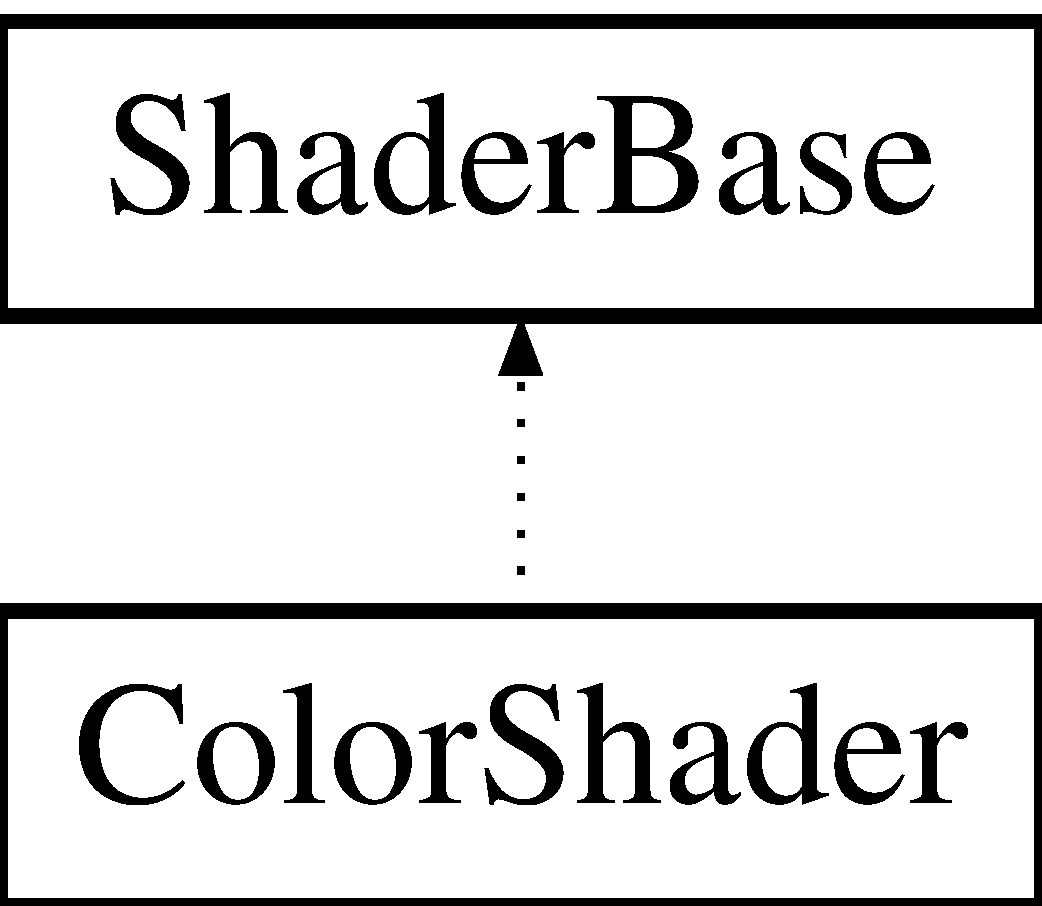
\includegraphics[height=2.000000cm]{classColorShader}
\end{center}
\end{figure}
\subsection*{\-Public \-Types}
\begin{DoxyCompactItemize}
\item 
enum \{ {\bfseries \-V\-E\-R\-T\-E\-X\-\_\-\-I\-N\-D\-E\-X} =  0, 
{\bfseries \-C\-O\-L\-O\-R\-\_\-\-I\-N\-D\-E\-X} =  1
 \}
\end{DoxyCompactItemize}
\subsection*{\-Public \-Member \-Functions}
\begin{DoxyCompactItemize}
\item 
\hypertarget{classColorShader_a4596a361346a800e9f62fe79f0dd6f6e}{void {\bfseries \-Enable\-Program} (void)}\label{classColorShader_a4596a361346a800e9f62fe79f0dd6f6e}

\item 
\hypertarget{classColorShader_a1643a96f4c036e02311080aef95573be}{void {\bfseries \-Disable\-Program} (void)}\label{classColorShader_a1643a96f4c036e02311080aef95573be}

\item 
\hypertarget{classColorShader_af6d90987d172f4501d1f0bd07cdb11a1}{void {\bfseries \-Model\-View} (const glm\-::mat4 \&)}\label{classColorShader_af6d90987d172f4501d1f0bd07cdb11a1}

\item 
\hypertarget{classColorShader_a58dd5bed84ed183352bdd722764d8111}{void {\bfseries \-Color} (const glm\-::vec4 \&)}\label{classColorShader_a58dd5bed84ed183352bdd722764d8111}

\item 
\hypertarget{classColorShader_a8e05747a087576897e925b780d602dc0}{void {\bfseries \-Projection} (const glm\-::mat4 \&)}\label{classColorShader_a8e05747a087576897e925b780d602dc0}

\end{DoxyCompactItemize}
\subsection*{\-Static \-Public \-Member \-Functions}
\begin{DoxyCompactItemize}
\item 
\hypertarget{classColorShader_a12a041a319bf5bb912074a10ab251d50}{static \hyperlink{classColorShader}{\-Color\-Shader} $\ast$ {\bfseries \-Make} (void)}\label{classColorShader_a12a041a319bf5bb912074a10ab251d50}

\end{DoxyCompactItemize}


\-The documentation for this class was generated from the following files\-:\begin{DoxyCompactItemize}
\item 
shaders/\-Color\-Shader.\-h\item 
shaders/\-Color\-Shader.\-cpp\end{DoxyCompactItemize}

\hypertarget{structCompareVertexDataf}{\section{\-Compare\-Vertex\-Dataf \-Struct \-Reference}
\label{structCompareVertexDataf}\index{\-Compare\-Vertex\-Dataf@{\-Compare\-Vertex\-Dataf}}
}
\subsection*{\-Public \-Member \-Functions}
\begin{DoxyCompactItemize}
\item 
\hypertarget{structCompareVertexDataf_ab5bcae7b72fb692d1d69d75bb0756c01}{bool {\bfseries operator()} (\hyperlink{structVertexDataf}{\-Vertex\-Dataf} $\ast$a, \hyperlink{structVertexDataf}{\-Vertex\-Dataf} $\ast$b)}\label{structCompareVertexDataf_ab5bcae7b72fb692d1d69d75bb0756c01}

\end{DoxyCompactItemize}


\-The documentation for this struct was generated from the following file\-:\begin{DoxyCompactItemize}
\item 
\-Chunk\-Object.\-cpp\end{DoxyCompactItemize}

\hypertarget{classstd_1_1condition__variable}{\section{std\-:\-:condition\-\_\-variable \-Class \-Reference}
\label{classstd_1_1condition__variable}\index{std\-::condition\-\_\-variable@{std\-::condition\-\_\-variable}}
}
\subsection*{\-Public \-Member \-Functions}
\begin{DoxyCompactItemize}
\item 
\hypertarget{classstd_1_1condition__variable_aac6917dec618a858a9c10dac6c858bf2}{void {\bfseries wait} (\hyperlink{classstd_1_1unique__lock}{unique\-\_\-lock}$<$ \hyperlink{classstd_1_1mutex}{mutex} $>$ \&lock)}\label{classstd_1_1condition__variable_aac6917dec618a858a9c10dac6c858bf2}

\item 
\hypertarget{classstd_1_1condition__variable_a543f0f32e56ccac6d758e6fa668581d5}{void {\bfseries notify\-\_\-all} (void)}\label{classstd_1_1condition__variable_a543f0f32e56ccac6d758e6fa668581d5}

\item 
\hypertarget{classstd_1_1condition__variable_a4942d1d35b1259eb35773b604e0be20a}{void {\bfseries notify\-\_\-one} (void)}\label{classstd_1_1condition__variable_a4942d1d35b1259eb35773b604e0be20a}

\end{DoxyCompactItemize}


\-The documentation for this class was generated from the following file\-:\begin{DoxyCompactItemize}
\item 
mythread.\-h\end{DoxyCompactItemize}

\hypertarget{classCube}{\section{\-Cube \-Class \-Reference}
\label{classCube}\index{\-Cube@{\-Cube}}
}
\subsection*{\-Public \-Member \-Functions}
\begin{DoxyCompactItemize}
\item 
\hypertarget{classCube_ab8eeecb48f43ca2e67ac62c4f5da4f1a}{void {\bfseries \-Init} (\hyperlink{classChunkShader}{\-Chunk\-Shader} $\ast$shader)}\label{classCube_ab8eeecb48f43ca2e67ac62c4f5da4f1a}

\item 
\hypertarget{classCube_a4951e9c17d20b7d47a45ea14cb839f9f}{void {\bfseries \-Draw} (void) const }\label{classCube_a4951e9c17d20b7d47a45ea14cb839f9f}

\item 
\hypertarget{classCube_a9e96713d2fec806f61a37c6d6c1628c1}{void {\bfseries \-Draw\-Lines} (void) const }\label{classCube_a9e96713d2fec806f61a37c6d6c1628c1}

\end{DoxyCompactItemize}


\-The documentation for this class was generated from the following files\-:\begin{DoxyCompactItemize}
\item 
shapes/\-Cube.\-h\item 
shapes/\-Cube.\-cpp\end{DoxyCompactItemize}

\hypertarget{classCylinder}{\section{\-Cylinder \-Class \-Reference}
\label{classCylinder}\index{\-Cylinder@{\-Cylinder}}
}
\subsection*{\-Public \-Member \-Functions}
\begin{DoxyCompactItemize}
\item 
\hypertarget{classCylinder_a5b973d84211110771ca06e8ee1527a0a}{void {\bfseries \-Init} (\hyperlink{classStageOneShader}{\-Stage\-One\-Shader} $\ast$shader, int num\-Segments)}\label{classCylinder_a5b973d84211110771ca06e8ee1527a0a}

\item 
\hypertarget{classCylinder_a712a1b1209889baea0d0d6e06f5be70e}{void {\bfseries \-Draw} (\hyperlink{classStageOneShader}{\-Stage\-One\-Shader} $\ast$shader) const }\label{classCylinder_a712a1b1209889baea0d0d6e06f5be70e}

\end{DoxyCompactItemize}


\-The documentation for this class was generated from the following files\-:\begin{DoxyCompactItemize}
\item 
shapes/\-Cylinder.\-h\item 
shapes/\-Cylinder.\-cpp\end{DoxyCompactItemize}

\hypertarget{structData}{\section{\-Data \-Struct \-Reference}
\label{structData}\index{\-Data@{\-Data}}
}
\subsection*{\-Public \-Attributes}
\begin{DoxyCompactItemize}
\item 
\hypertarget{structData_abeda0dab8e22c6b41b9e3e19f0665524}{glm\-::mat4 {\bfseries projectionmatrix}}\label{structData_abeda0dab8e22c6b41b9e3e19f0665524}

\item 
\hypertarget{structData_a1db0d7b30c27fc1ada74baf396f621ad}{glm\-::mat4 {\bfseries projectionviewmatrix}}\label{structData_a1db0d7b30c27fc1ada74baf396f621ad}

\item 
\hypertarget{structData_a8769f1fa97b23d614092404fc92c768e}{glm\-::mat4 {\bfseries viewmatrix}}\label{structData_a8769f1fa97b23d614092404fc92c768e}

\item 
\hypertarget{structData_aac1243b77cd89649a159926c76e41e21}{glm\-::vec4 {\bfseries camera}}\label{structData_aac1243b77cd89649a159926c76e41e21}

\item 
\hypertarget{structData_a64bcfa2de4f541f2e78e07783ff54493}{float {\bfseries viewingdistance}}\label{structData_a64bcfa2de4f541f2e78e07783ff54493}

\item 
\hypertarget{structData_af6a336d6a6c82227053ff5540aa94526}{int {\bfseries performance}}\label{structData_af6a336d6a6c82227053ff5540aa94526}

\item 
\hypertarget{structData_a8fef884a97064a497f1f61e92a496d86}{int {\bfseries dynamicshadows}}\label{structData_a8fef884a97064a497f1f61e92a496d86}

\item 
\hypertarget{structData_a8e994d240a8122b9aa9e90bf6cb20912}{int {\bfseries windowheight}}\label{structData_a8e994d240a8122b9aa9e90bf6cb20912}

\item 
\hypertarget{structData_ad6771abcfa9848313a4da92d2de6a0ca}{int {\bfseries toggle\-Testing}}\label{structData_ad6771abcfa9848313a4da92d2de6a0ca}

\item 
\hypertarget{structData_a9ab88fa045dc69ac62a085ae8e506997}{float {\bfseries exposure}}\label{structData_a9ab88fa045dc69ac62a085ae8e506997}

\item 
\hypertarget{structData_ab4ebab84b52d9b6a9f7010d3cbee39f2}{float {\bfseries ambient\-Light}}\label{structData_ab4ebab84b52d9b6a9f7010d3cbee39f2}

\end{DoxyCompactItemize}


\-The documentation for this struct was generated from the following file\-:\begin{DoxyCompactItemize}
\item 
uniformbuffer.\-cpp\end{DoxyCompactItemize}

\hypertarget{classDeferredLighting}{\section{\-Deferred\-Lighting \-Class \-Reference}
\label{classDeferredLighting}\index{\-Deferred\-Lighting@{\-Deferred\-Lighting}}
}
\-Inheritance diagram for \-Deferred\-Lighting\-:\begin{figure}[H]
\begin{center}
\leavevmode
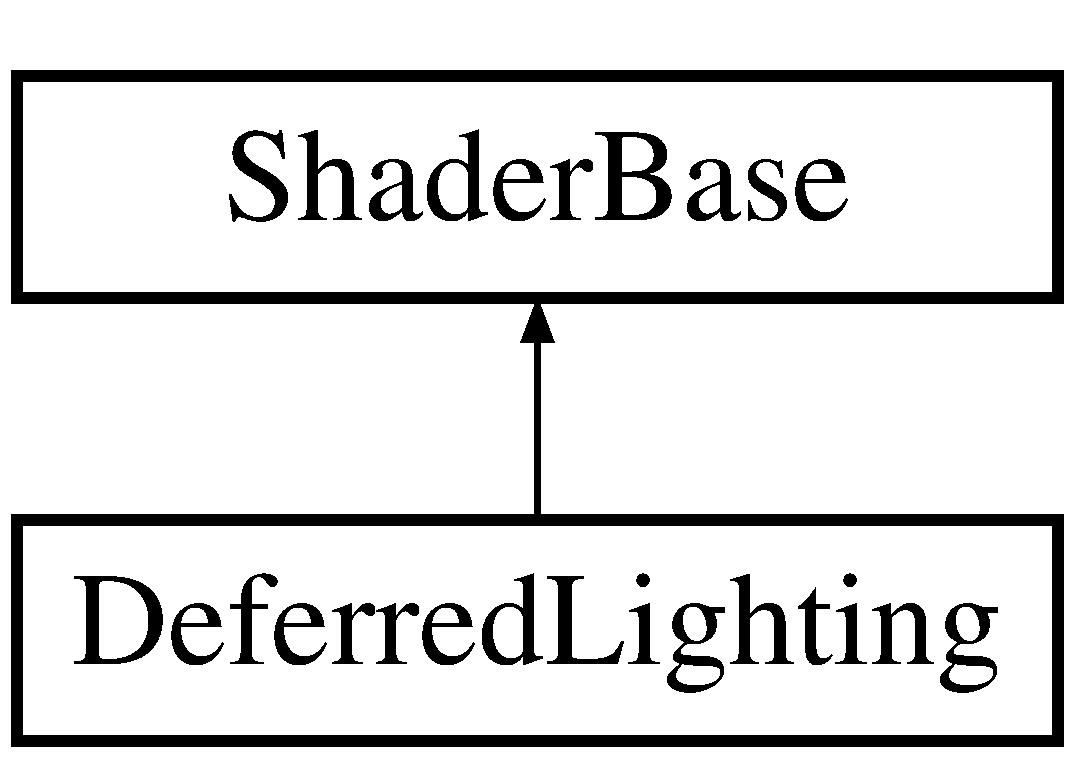
\includegraphics[height=2.000000cm]{classDeferredLighting}
\end{center}
\end{figure}
\subsection*{\-Public \-Member \-Functions}
\begin{DoxyCompactItemize}
\item 
\hypertarget{classDeferredLighting_a7f972ae0f3b0d0abf541ff828fb29271}{void {\bfseries \-Init} (void)}\label{classDeferredLighting_a7f972ae0f3b0d0abf541ff828fb29271}

\item 
\hypertarget{classDeferredLighting_adbf5ea22dfe764a11fc5bcfbeb44f6e4}{void {\bfseries \-Enable\-Program} (void)}\label{classDeferredLighting_adbf5ea22dfe764a11fc5bcfbeb44f6e4}

\item 
\hypertarget{classDeferredLighting_a9e234f5c7f64a8451928a4e5cf9384ec}{void {\bfseries \-Disable\-Program} (void)}\label{classDeferredLighting_a9e234f5c7f64a8451928a4e5cf9384ec}

\item 
\hypertarget{classDeferredLighting_aea9c2f20b4b3f1bf31bbaf53f4bb915b}{void {\bfseries \-Vertex\-Attrib\-Pointer} (\-G\-Lenum type, \-G\-Lsizei stride, const \-G\-Lvoid $\ast$pointer)}\label{classDeferredLighting_aea9c2f20b4b3f1bf31bbaf53f4bb915b}

\item 
\hypertarget{classDeferredLighting_afe628eaa8d7bd6025cfceae03cc0d181}{void {\bfseries \-Player\-Dead} (bool)}\label{classDeferredLighting_afe628eaa8d7bd6025cfceae03cc0d181}

\item 
\hypertarget{classDeferredLighting_aee0f2239692678c0f6a5cd16dda8a6ef}{void {\bfseries \-In\-Water} (bool)}\label{classDeferredLighting_aee0f2239692678c0f6a5cd16dda8a6ef}

\item 
\hypertarget{classDeferredLighting_aab381b529dd77f5b6a8cc392a6ae5599}{void {\bfseries \-Inside\-Teleport} (bool flag)}\label{classDeferredLighting_aab381b529dd77f5b6a8cc392a6ae5599}

\item 
\hypertarget{classDeferredLighting_a57271d2a1f3d1d0b20b19b7c1459a501}{void {\bfseries \-Set\-White\-Point} (float)}\label{classDeferredLighting_a57271d2a1f3d1d0b20b19b7c1459a501}

\item 
\hypertarget{classDeferredLighting_a0a34210e2cee2b77afb1805e63ef50b4}{void {\bfseries \-Draw} ()}\label{classDeferredLighting_a0a34210e2cee2b77afb1805e63ef50b4}

\end{DoxyCompactItemize}


\-The documentation for this class was generated from the following files\-:\begin{DoxyCompactItemize}
\item 
shaders/\-Deferred\-Lighting.\-h\item 
shaders/\-Deferred\-Lighting.\-cpp\end{DoxyCompactItemize}

\hypertarget{classDrawFont}{\section{\-Draw\-Font \-Class \-Reference}
\label{classDrawFont}\index{\-Draw\-Font@{\-Draw\-Font}}
}
\subsection*{\-Public \-Member \-Functions}
\begin{DoxyCompactItemize}
\item 
\hypertarget{classDrawFont_ab65062370529725d0bd8d3da80356b9c}{void {\bfseries \-Update\-Projection} (void)}\label{classDrawFont_ab65062370529725d0bd8d3da80356b9c}

\item 
\hypertarget{classDrawFont_a043f1ae634caac4a82e6e725a14e4a71}{void {\bfseries \-Set\-Offset} (float row, float col)}\label{classDrawFont_a043f1ae634caac4a82e6e725a14e4a71}

\item 
\hypertarget{classDrawFont_a0b97262ce99de92a639ccc44bf38fc55}{void {\bfseries \-Enable} (void)}\label{classDrawFont_a0b97262ce99de92a639ccc44bf38fc55}

\item 
\hypertarget{classDrawFont_a258f44fb5bac847546eb4ec963d88144}{void {\bfseries \-Disable} (void)}\label{classDrawFont_a258f44fb5bac847546eb4ec963d88144}

\item 
\hypertarget{classDrawFont_a432fb290d8f91bcf91a809ab0d6d147b}{void {\bfseries \-Init} (const std\-::string \&font\-Name)}\label{classDrawFont_a432fb290d8f91bcf91a809ab0d6d147b}

\end{DoxyCompactItemize}
\subsection*{\-Public \-Attributes}
\begin{DoxyCompactItemize}
\item 
\hypertarget{classDrawFont_a15cbb37666cd5d3cc7826df778caec30}{\-V\-S\-F\-L\-Font {\bfseries vsfl}}\label{classDrawFont_a15cbb37666cd5d3cc7826df778caec30}

\end{DoxyCompactItemize}


\-The documentation for this class was generated from the following files\-:\begin{DoxyCompactItemize}
\item 
\-Draw\-Text.\-h\item 
\-Draw\-Text.\-cpp\end{DoxyCompactItemize}

\hypertarget{structDrawObjectList}{\section{\-Draw\-Object\-List \-Struct \-Reference}
\label{structDrawObjectList}\index{\-Draw\-Object\-List@{\-Draw\-Object\-List}}
}
\subsection*{\-Public \-Member \-Functions}
\begin{DoxyCompactItemize}
\item 
\hypertarget{structDrawObjectList_a4f04a3efb4d346ec439413b60a60f735}{{\bfseries \-Draw\-Object\-List} (glm\-::vec3 p, unsigned char t)}\label{structDrawObjectList_a4f04a3efb4d346ec439413b60a60f735}

\end{DoxyCompactItemize}
\subsection*{\-Public \-Attributes}
\begin{DoxyCompactItemize}
\item 
\hypertarget{structDrawObjectList_a30b18bb8b60c5fe3135512468550236c}{glm\-::vec3 {\bfseries pos}}\label{structDrawObjectList_a30b18bb8b60c5fe3135512468550236c}

\item 
\hypertarget{structDrawObjectList_a8486a79ce9e68f04cd71ac2c0eff3f1e}{unsigned char {\bfseries type}}\label{structDrawObjectList_a8486a79ce9e68f04cd71ac2c0eff3f1e}

\end{DoxyCompactItemize}


\-The documentation for this struct was generated from the following file\-:\begin{DoxyCompactItemize}
\item 
render.\-h\end{DoxyCompactItemize}

\hypertarget{classDrawTexture}{\section{\-Draw\-Texture \-Class \-Reference}
\label{classDrawTexture}\index{\-Draw\-Texture@{\-Draw\-Texture}}
}
\subsection*{\-Public \-Member \-Functions}
\begin{DoxyCompactItemize}
\item 
\hypertarget{classDrawTexture_a3a75c8540a457dde0ef60d192cc38230}{void {\bfseries \-Draw} (const glm\-::mat4 \&projection, const glm\-::mat4 \&model, float alpha=1.\-0f) const }\label{classDrawTexture_a3a75c8540a457dde0ef60d192cc38230}

\item 
\hypertarget{classDrawTexture_a6bfd29bc989d7a4e0699c6db99fdaa67}{void {\bfseries \-Draw\-Offset} (const glm\-::mat4 \&projection, const glm\-::mat4 \&model, float offs\-X, float offs\-Y, float mult) const }\label{classDrawTexture_a6bfd29bc989d7a4e0699c6db99fdaa67}

\item 
\hypertarget{classDrawTexture_acab4508f074e7b90b40a9ec810a7788f}{void {\bfseries \-Draw\-Depth} (const glm\-::mat4 \&projection, const glm\-::mat4 \&model, float offs\-X, float offs\-Y, float mult) const }\label{classDrawTexture_acab4508f074e7b90b40a9ec810a7788f}

\item 
\hypertarget{classDrawTexture_a717ebdf22de74b71b4d2fc540ed9a7bb}{void {\bfseries \-Draw\-Basic} (void) const }\label{classDrawTexture_a717ebdf22de74b71b4d2fc540ed9a7bb}

\end{DoxyCompactItemize}
\subsection*{\-Static \-Public \-Member \-Functions}
\begin{DoxyCompactItemize}
\item 
\hypertarget{classDrawTexture_a40421b54de7ae286e9017264d558d902}{static \hyperlink{classDrawTexture}{\-Draw\-Texture} $\ast$ {\bfseries \-Make} (void)}\label{classDrawTexture_a40421b54de7ae286e9017264d558d902}

\end{DoxyCompactItemize}


\-The documentation for this class was generated from the following files\-:\begin{DoxyCompactItemize}
\item 
\-Draw\-Texture.\-h\item 
\-Draw\-Texture.\-cpp\end{DoxyCompactItemize}

\hypertarget{classFogs}{\section{\-Fogs \-Class \-Reference}
\label{classFogs}\index{\-Fogs@{\-Fogs}}
}
\subsection*{\-Public \-Member \-Functions}
\begin{DoxyCompactItemize}
\item 
\hypertarget{classFogs_acafeea155d5753f71df0e6a9157a068c}{void {\bfseries \-Clear} (void)}\label{classFogs_acafeea155d5753f71df0e6a9157a068c}

\item 
\hypertarget{classFogs_a725dd132babc2d7b11ae57f07a31c634}{void {\bfseries \-Add} (float x, float y, float z, int radius, float ambient)}\label{classFogs_a725dd132babc2d7b11ae57f07a31c634}

\item 
\hypertarget{classFogs_acd0a7cb6b48b41420fa684fca82e7c38}{int {\bfseries \-Get\-Count} (void) const }\label{classFogs_acd0a7cb6b48b41420fa684fca82e7c38}

\item 
\hypertarget{classFogs_aaf0ffe1147111dde7ddc16ce4d85d5f5}{glm\-::vec4 $\ast$ {\bfseries \-Get\-List} (void)}\label{classFogs_aaf0ffe1147111dde7ddc16ce4d85d5f5}

\end{DoxyCompactItemize}


\-The documentation for this class was generated from the following files\-:\begin{DoxyCompactItemize}
\item 
render.\-h\item 
render.\-cpp\end{DoxyCompactItemize}

\hypertarget{classgameDialog}{\section{game\-Dialog \-Class \-Reference}
\label{classgameDialog}\index{game\-Dialog@{game\-Dialog}}
}
\subsection*{\-Public \-Types}
\begin{DoxyCompactItemize}
\item 
enum {\bfseries \-Calibration} \{ {\bfseries \-C\-A\-L\-I\-B\-\_\-\-E\-X\-P\-O\-S\-U\-R\-E}, 
{\bfseries \-C\-A\-L\-I\-B\-\_\-\-W\-H\-I\-T\-E\-\_\-\-P\-O\-I\-N\-T}, 
{\bfseries \-C\-A\-L\-I\-B\-\_\-\-A\-M\-B\-I\-E\-N\-T}, 
{\bfseries \-C\-A\-L\-I\-B\-\_\-\-N\-O\-N\-E}
 \}
\item 
enum {\bfseries \-Effect} \{ {\bfseries \-E\-F\-F\-E\-C\-T\-\_\-\-N\-O\-N\-E}, 
{\bfseries \-E\-F\-F\-E\-C\-T\-\_\-\-Z\-O\-O\-M1}, 
{\bfseries \-E\-F\-F\-E\-C\-T\-\_\-\-Z\-O\-O\-M2}
 \}
\end{DoxyCompactItemize}
\subsection*{\-Public \-Member \-Functions}
\begin{DoxyCompactItemize}
\item 
\hypertarget{classgameDialog_a21cedaedca966f952c37ae934b9ce4fa}{void {\bfseries render} ()}\label{classgameDialog_a21cedaedca966f952c37ae934b9ce4fa}

\item 
\hypertarget{classgameDialog_a4a83e9132cfa2201973f5e65ed0f92fc}{void {\bfseries init} ()}\label{classgameDialog_a4a83e9132cfa2201973f5e65ed0f92fc}

\item 
\hypertarget{classgameDialog_a5d6531dc2cfad024519f7725a7ee5c16}{void {\bfseries handle\-Mouse} (int button, int action)}\label{classgameDialog_a5d6531dc2cfad024519f7725a7ee5c16}

\item 
\hypertarget{classgameDialog_a8776daec36b7ff7115c7099dd25cd3e0}{void {\bfseries \-Update} ()}\label{classgameDialog_a8776daec36b7ff7115c7099dd25cd3e0}

\item 
\hypertarget{classgameDialog_aa8d320eca21fe0eb93d7dfed918b73cf}{void {\bfseries \-Set\-Message} (const char $\ast$)}\label{classgameDialog_aa8d320eca21fe0eb93d7dfed918b73cf}

\item 
\hypertarget{classgameDialog_a90c0dcab2347b83964aa424104b7b3bf}{void {\bfseries \-Handle\-Key\-Release} (int key)}\label{classgameDialog_a90c0dcab2347b83964aa424104b7b3bf}

\item 
\hypertarget{classgameDialog_a2ccd78496d884bff62eecda57accfbd2}{void {\bfseries \-Handle\-Key\-Press} (int key)}\label{classgameDialog_a2ccd78496d884bff62eecda57accfbd2}

\item 
\hypertarget{classgameDialog_a4ace469010b65e89c2cb8d7fedcfbbe3}{void {\bfseries \-Handle\-Character} (int key, int action)}\label{classgameDialog_a4ace469010b65e89c2cb8d7fedcfbbe3}

\item 
\hypertarget{classgameDialog_a22384496d1e9d31a02fc8ac2c0c9037c}{void {\bfseries handle\-Resize} (int w, int h)}\label{classgameDialog_a22384496d1e9d31a02fc8ac2c0c9037c}

\item 
\hypertarget{classgameDialog_a70e553f6ff6baace3a4c8f4ba6be0ebd}{void {\bfseries handle\-Mouse\-Active\-Motion} (int x, int y)}\label{classgameDialog_a70e553f6ff6baace3a4c8f4ba6be0ebd}

\item 
\hypertarget{classgameDialog_a48b2f2b50db4bcd7bb5d859aa6731b07}{void {\bfseries \-Click\-On\-Block} (int x, int y)}\label{classgameDialog_a48b2f2b50db4bcd7bb5d859aa6731b07}

\item 
\hypertarget{classgameDialog_a0dc52082ffdd613057d57507b0f5f753}{void {\bfseries \-Click\-On\-Object} (int x, int y)}\label{classgameDialog_a0dc52082ffdd613057d57507b0f5f753}

\item 
\hypertarget{classgameDialog_abc1d0acda84d792d8c0bb3910bdc04d8}{void {\bfseries \-Attach\-Block\-To\-Surface} (int row, int col)}\label{classgameDialog_abc1d0acda84d792d8c0bb3910bdc04d8}

\item 
\hypertarget{classgameDialog_a1c0d45b906334858deb4c24ebe9685ab}{void {\bfseries \-Clear\-Selection} (void)}\label{classgameDialog_a1c0d45b906334858deb4c24ebe9685ab}

\item 
\hypertarget{classgameDialog_ae0dfad988d09e9b9fef312439c38ac13}{void {\bfseries \-Aggro\-From} (\hyperlink{classObject}{\-Object} $\ast$)}\label{classgameDialog_ae0dfad988d09e9b9fef312439c38ac13}

\item 
\hypertarget{classgameDialog_a578ed50dff9baa0c1751664c62c3feb9}{void {\bfseries \-Calibrate\-Mode} (\-Calibration)}\label{classgameDialog_a578ed50dff9baa0c1751664c62c3feb9}

\item 
\hypertarget{classgameDialog_ab99cb133d972356394df9a542f447ac7}{bool {\bfseries \-Third\-Person\-View} (void) const }\label{classgameDialog_ab99cb133d972356394df9a542f447ac7}

\item 
\hypertarget{classgameDialog_a9c0f282acabaab02ce168eb5d7b17327}{void {\bfseries \-Update\-Running\-Status} (bool disable)}\label{classgameDialog_a9c0f282acabaab02ce168eb5d7b17327}

\item 
\hypertarget{classgameDialog_a46ef262050295e930cd010ef0a7bf13f}{void {\bfseries \-Request\-Effect} (\-Effect eff)}\label{classgameDialog_a46ef262050295e930cd010ef0a7bf13f}

\item 
\hypertarget{classgameDialog_a8ceb2b685ea0de987194b22e5ae6fc8b}{void {\bfseries \-Cancel\-Current\-Effect} (void)}\label{classgameDialog_a8ceb2b685ea0de987194b22e5ae6fc8b}

\item 
\hypertarget{classgameDialog_ab095c6cac56d552e8b3a07511f1e2f3a}{void {\bfseries \-Update\-Effect} (void)}\label{classgameDialog_ab095c6cac56d552e8b3a07511f1e2f3a}

\item 
\hypertarget{classgameDialog_a6f84b2a49df351b6e9153a29aa342529}{void {\bfseries \-Clear\-Input\-Redirect} (void)}\label{classgameDialog_a6f84b2a49df351b6e9153a29aa342529}

\end{DoxyCompactItemize}
\subsection*{\-Public \-Attributes}
\begin{DoxyCompactItemize}
\item 
\hypertarget{classgameDialog_a4ad8cad61bb9109745936ec02a29e4df}{bool {\bfseries f\-Show\-Inventory}}\label{classgameDialog_a4ad8cad61bb9109745936ec02a29e4df}

\end{DoxyCompactItemize}


\-The documentation for this class was generated from the following files\-:\begin{DoxyCompactItemize}
\item 
gamedialog.\-h\item 
gamedialog.\-cpp\end{DoxyCompactItemize}

\hypertarget{classGameMode}{\section{\-Game\-Mode \-Class \-Reference}
\label{classGameMode}\index{\-Game\-Mode@{\-Game\-Mode}}
}
\subsection*{\-Public \-Types}
\begin{DoxyCompactItemize}
\item 
enum {\bfseries \-Mode} \{ \*
{\bfseries \-I\-N\-I\-T}, 
{\bfseries \-L\-O\-G\-I\-N}, 
{\bfseries \-R\-E\-Q\-\_\-\-P\-A\-S\-S\-W\-D}, 
{\bfseries \-P\-A\-S\-S\-W\-O\-R\-D}, 
\*
{\bfseries \-W\-A\-I\-T\-\_\-\-A\-C\-K}, 
{\bfseries \-L\-O\-G\-I\-N\-\_\-\-F\-A\-I\-L\-E\-D}, 
{\bfseries \-G\-A\-M\-E}, 
{\bfseries \-C\-O\-N\-S\-T\-R\-U\-C\-T}, 
\*
{\bfseries \-T\-E\-L\-E\-P\-O\-R\-T}, 
{\bfseries \-E\-S\-C}, 
{\bfseries \-E\-X\-I\-T}
 \}
\end{DoxyCompactItemize}
\subsection*{\-Public \-Member \-Functions}
\begin{DoxyCompactItemize}
\item 
\hypertarget{classGameMode_a4193e0de55c1aa7a4625901cf8540c3a}{void {\bfseries \-Set} (\-Mode)}\label{classGameMode_a4193e0de55c1aa7a4625901cf8540c3a}

\item 
\hypertarget{classGameMode_a173095ce765ae09f52a3f771a5fb1826}{\-Mode {\bfseries \-Get} (void) const }\label{classGameMode_a173095ce765ae09f52a3f771a5fb1826}

\item 
\hypertarget{classGameMode_aa3b815262ac868c178bf22e959b4fdf4}{bool {\bfseries \-Communication\-Allowed} (void) const }\label{classGameMode_aa3b815262ac868c178bf22e959b4fdf4}

\end{DoxyCompactItemize}


\-The documentation for this class was generated from the following files\-:\begin{DoxyCompactItemize}
\item 
modes.\-h\item 
modes.\-cpp\end{DoxyCompactItemize}

\hypertarget{structGameTexture}{\section{\-Game\-Texture \-Struct \-Reference}
\label{structGameTexture}\index{\-Game\-Texture@{\-Game\-Texture}}
}
\subsection*{\-Static \-Public \-Member \-Functions}
\begin{DoxyCompactItemize}
\item 
\hypertarget{structGameTexture_a0e9bf994207d7b2e4c24e742a1dda361}{static void {\bfseries \-Init} (void)}\label{structGameTexture_a0e9bf994207d7b2e4c24e742a1dda361}

\item 
\hypertarget{structGameTexture_a686f11f41c5629e865503829e925563b}{static const \hyperlink{structGameTexture}{\-Game\-Texture} $\ast$ {\bfseries \-Get\-Game\-Texture} (int index)}\label{structGameTexture_a686f11f41c5629e865503829e925563b}

\end{DoxyCompactItemize}
\subsection*{\-Public \-Attributes}
\begin{DoxyCompactItemize}
\item 
\hypertarget{structGameTexture_afbbbbb40772be9d8efd7a9745c51fc5f}{int {\bfseries bl\-Type}}\label{structGameTexture_afbbbbb40772be9d8efd7a9745c51fc5f}

\item 
\hypertarget{structGameTexture_a3982258556ec5b47c9feb7c588ccb999}{\-G\-Luint {\bfseries id}}\label{structGameTexture_a3982258556ec5b47c9feb7c588ccb999}

\item 
\hypertarget{structGameTexture_a3fe982d67133975c95dd3bf920fef66b}{const char $\ast$ {\bfseries file\-Name}}\label{structGameTexture_a3fe982d67133975c95dd3bf920fef66b}

\item 
\hypertarget{structGameTexture_ad1a245011045fd8af37be8f604b80e93}{const char $\ast$ {\bfseries descr}}\label{structGameTexture_ad1a245011045fd8af37be8f604b80e93}

\item 
\hypertarget{structGameTexture_adbb8cf75f8fd60c01ab9f9de4eca36ac}{unsigned {\bfseries flag}}\label{structGameTexture_adbb8cf75f8fd60c01ab9f9de4eca36ac}

\end{DoxyCompactItemize}
\subsection*{\-Static \-Public \-Attributes}
\begin{DoxyCompactItemize}
\item 
\hypertarget{structGameTexture_a2eb4e1f8b49df08bab6da38010dcac69}{static \-G\-Luint {\bfseries \-Grass\-Texture\-Id}}\label{structGameTexture_a2eb4e1f8b49df08bab6da38010dcac69}

\item 
\hypertarget{structGameTexture_a936c6c7146ba919be51f8f3c33777225}{static \-G\-Luint {\bfseries \-Tuft\-Of\-Grass}}\label{structGameTexture_a936c6c7146ba919be51f8f3c33777225}

\item 
\hypertarget{structGameTexture_a159d393ceca2ed1b6d9b470844698c50}{static \-G\-Luint {\bfseries \-Flowers}}\label{structGameTexture_a159d393ceca2ed1b6d9b470844698c50}

\item 
\hypertarget{structGameTexture_a2c28a6a26068c37ea3b1f33eb6393eda}{static \-G\-Luint {\bfseries \-Leaf\-Texture\-Id}}\label{structGameTexture_a2c28a6a26068c37ea3b1f33eb6393eda}

\item 
\hypertarget{structGameTexture_acaf71d22e769c12f8ada73d748f54386}{static \-G\-Luint {\bfseries \-Stone\-Texture2\-Id}}\label{structGameTexture_acaf71d22e769c12f8ada73d748f54386}

\item 
\hypertarget{structGameTexture_a2d646a68617fcd389749951b5e2b0e7e}{static \-G\-Luint {\bfseries \-Ladder\-On\-Stone}}\label{structGameTexture_a2d646a68617fcd389749951b5e2b0e7e}

\item 
\hypertarget{structGameTexture_ad647eb8e713a5552739b9362a7cbd53f}{static \-G\-Luint {\bfseries \-Tree\-Bark\-Id}}\label{structGameTexture_ad647eb8e713a5552739b9362a7cbd53f}

\item 
\hypertarget{structGameTexture_a55c73e92a176db210d7785ba81b6d00f}{static \-G\-Luint {\bfseries \-Hedge}}\label{structGameTexture_a55c73e92a176db210d7785ba81b6d00f}

\item 
\hypertarget{structGameTexture_af3050a255c271887c6cabb5736263faf}{static \-G\-Luint {\bfseries \-Window}}\label{structGameTexture_af3050a255c271887c6cabb5736263faf}

\item 
\hypertarget{structGameTexture_a744d4915cd7cd9458e854dc0031cc250}{static \-G\-Luint {\bfseries \-Snow}}\label{structGameTexture_a744d4915cd7cd9458e854dc0031cc250}

\item 
\hypertarget{structGameTexture_aebac9cd660f568ae8bc963766073fe09}{static \-G\-Luint {\bfseries \-Branch}}\label{structGameTexture_aebac9cd660f568ae8bc963766073fe09}

\item 
\hypertarget{structGameTexture_a201b1141a82a309a94dccb5ede8bbb51}{static \-G\-Luint {\bfseries \-Sky1\-Id}}\label{structGameTexture_a201b1141a82a309a94dccb5ede8bbb51}

\item 
\hypertarget{structGameTexture_afdf45bd48374dcc9b4b5afd31fc9a6e5}{static \-G\-Luint {\bfseries \-Sky2\-Id}}\label{structGameTexture_afdf45bd48374dcc9b4b5afd31fc9a6e5}

\item 
\hypertarget{structGameTexture_a1852440744012e62ac001fe2baf2f4ef}{static \-G\-Luint {\bfseries \-Sky3\-Id}}\label{structGameTexture_a1852440744012e62ac001fe2baf2f4ef}

\item 
\hypertarget{structGameTexture_a707f439485b939188c40b121cf44ca10}{static \-G\-Luint {\bfseries \-Sky4\-Id}}\label{structGameTexture_a707f439485b939188c40b121cf44ca10}

\item 
\hypertarget{structGameTexture_a4cb16ead98130bdcf3786b37fe8282be}{static \-G\-Luint {\bfseries \-Skyup\-Id}}\label{structGameTexture_a4cb16ead98130bdcf3786b37fe8282be}

\item 
\hypertarget{structGameTexture_a9ddb5233592588f5b734cbb5778d5aa7}{static \-G\-Luint {\bfseries \-Red\-Scales\-Id}}\label{structGameTexture_a9ddb5233592588f5b734cbb5778d5aa7}

\item 
\hypertarget{structGameTexture_aaa5a5b8e0ed3d5acbf62fe4de017222e}{static \-G\-Luint {\bfseries \-Morran}}\label{structGameTexture_aaa5a5b8e0ed3d5acbf62fe4de017222e}

\item 
\hypertarget{structGameTexture_a1b269c6f3458a79183b0cf556126d923}{static \-G\-Luint {\bfseries \-Fur1\-Id}}\label{structGameTexture_a1b269c6f3458a79183b0cf556126d923}

\item 
\hypertarget{structGameTexture_a7ba59e62a9c149b2eb4df2f2b4c5afa6}{static \-G\-Luint {\bfseries \-Monster\-Face1}}\label{structGameTexture_a7ba59e62a9c149b2eb4df2f2b4c5afa6}

\item 
\hypertarget{structGameTexture_ab0d00c7f45e1266445c54653b12cae93}{static \-G\-Luint {\bfseries \-Lantern\-Side\-Id}}\label{structGameTexture_ab0d00c7f45e1266445c54653b12cae93}

\item 
\hypertarget{structGameTexture_ab5b1578cc1a23510d4fee983db51d0bd}{static \-G\-Luint {\bfseries \-Teleport}}\label{structGameTexture_ab5b1578cc1a23510d4fee983db51d0bd}

\item 
\hypertarget{structGameTexture_acdb07c7a069c4a14d2e06d49b653e7c3}{static \-G\-Luint {\bfseries \-Light\-Balls\-Heal}}\label{structGameTexture_acdb07c7a069c4a14d2e06d49b653e7c3}

\item 
\hypertarget{structGameTexture_a3f5f21a12067e53ebfe176ba68dc3db3}{static \-G\-Luint {\bfseries \-Inventory\-Id}}\label{structGameTexture_a3f5f21a12067e53ebfe176ba68dc3db3}

\item 
\hypertarget{structGameTexture_a049c46a68be0310b3672833af68433e6}{static \-G\-Luint {\bfseries \-Equipment\-Id}}\label{structGameTexture_a049c46a68be0310b3672833af68433e6}

\item 
\hypertarget{structGameTexture_af2d6d25c527d451cdbb81534b6a4d6cb}{static \-G\-Luint {\bfseries \-Player\-Face} \mbox{[}5\mbox{]}}\label{structGameTexture_af2d6d25c527d451cdbb81534b6a4d6cb}

\item 
\hypertarget{structGameTexture_a8de26523d7d5e75aaf1b2ea9f21c8493}{static \-G\-Luint {\bfseries \-Red\-Color}}\label{structGameTexture_a8de26523d7d5e75aaf1b2ea9f21c8493}

\item 
\hypertarget{structGameTexture_a0561964878739a455915a2db303a92ba}{static \-G\-Luint {\bfseries \-Green\-Color}}\label{structGameTexture_a0561964878739a455915a2db303a92ba}

\item 
\hypertarget{structGameTexture_a6f7f621c6d240ae561cf244baf44eb0e}{static \-G\-Luint {\bfseries \-Blue\-Color}}\label{structGameTexture_a6f7f621c6d240ae561cf244baf44eb0e}

\item 
\hypertarget{structGameTexture_ad96c64a956bf5b0e68426e01ab40212c}{static \-G\-Luint {\bfseries \-Dark\-Gray}}\label{structGameTexture_ad96c64a956bf5b0e68426e01ab40212c}

\item 
\hypertarget{structGameTexture_a3f7c7c3c213990d3573428b48d0bc1d5}{static \-G\-Luint {\bfseries \-Red\-Chunk\-Border}}\label{structGameTexture_a3f7c7c3c213990d3573428b48d0bc1d5}

\item 
\hypertarget{structGameTexture_adc2c2d5dc0a5f3a7300b0c04f6ba3aad}{static \-G\-Luint {\bfseries \-Blue\-Chunk\-Border}}\label{structGameTexture_adc2c2d5dc0a5f3a7300b0c04f6ba3aad}

\item 
\hypertarget{structGameTexture_afed32cc2cb6180c330e41d2a318adbfe}{static \-G\-Luint {\bfseries \-Green\-Chunk\-Border}}\label{structGameTexture_afed32cc2cb6180c330e41d2a318adbfe}

\item 
\hypertarget{structGameTexture_abb657dad8dd2ff2e7eb52ee10bd86645}{static \-G\-Luint {\bfseries \-Compass\-Rose}}\label{structGameTexture_abb657dad8dd2ff2e7eb52ee10bd86645}

\item 
\hypertarget{structGameTexture_a3f1081ccdffa0131569f82f6536f9fe4}{static \-G\-Luint {\bfseries \-Damage\-Indication}}\label{structGameTexture_a3f1081ccdffa0131569f82f6536f9fe4}

\item 
\hypertarget{structGameTexture_ae18a404059333ec5998ec922085cc0d9}{static \-G\-Luint {\bfseries \-Texture\-Block}}\label{structGameTexture_ae18a404059333ec5998ec922085cc0d9}

\item 
\hypertarget{structGameTexture_ade9922cf2bf8504b4be3cd223f89da34}{static \-G\-Luint {\bfseries \-W\-E\-P1}}\label{structGameTexture_ade9922cf2bf8504b4be3cd223f89da34}

\item 
\hypertarget{structGameTexture_ad9c2ea17fda099c0c93467653bd4c2e5}{static \-G\-Luint {\bfseries \-W\-E\-P2}}\label{structGameTexture_ad9c2ea17fda099c0c93467653bd4c2e5}

\item 
\hypertarget{structGameTexture_ab812e6f0b9b903a684d06a8639e3e9ba}{static \-G\-Luint {\bfseries \-W\-E\-P3}}\label{structGameTexture_ab812e6f0b9b903a684d06a8639e3e9ba}

\item 
\hypertarget{structGameTexture_a76b8f5ab894134ca3e71bfe995bb4816}{static \-G\-Luint {\bfseries \-W\-E\-P4}}\label{structGameTexture_a76b8f5ab894134ca3e71bfe995bb4816}

\item 
\hypertarget{structGameTexture_a4ec826f487c9a94b2d5c1e7fefab3426}{static \-G\-Luint {\bfseries \-W\-E\-P1\-Text}}\label{structGameTexture_a4ec826f487c9a94b2d5c1e7fefab3426}

\item 
\hypertarget{structGameTexture_a4a8dced03cb4d8f8832c3acebad99e7e}{static \-G\-Luint {\bfseries \-W\-E\-P2\-Text}}\label{structGameTexture_a4a8dced03cb4d8f8832c3acebad99e7e}

\item 
\hypertarget{structGameTexture_a8ec2feb1898f8fa6a1d62fd3280b6c6c}{static \-G\-Luint {\bfseries \-W\-E\-P3\-Text}}\label{structGameTexture_a8ec2feb1898f8fa6a1d62fd3280b6c6c}

\item 
\hypertarget{structGameTexture_a591842d567b7793b42b6cf65bda489e3}{static \-G\-Luint {\bfseries \-W\-E\-P4\-Text}}\label{structGameTexture_a591842d567b7793b42b6cf65bda489e3}

\item 
\hypertarget{structGameTexture_aebbfe109cdf176674709c4d77ff47750}{static \-G\-Luint {\bfseries \-Coin}}\label{structGameTexture_aebbfe109cdf176674709c4d77ff47750}

\item 
\hypertarget{structGameTexture_a60e1e987f07d864e6de7bbb014c90ed4}{static \-G\-Luint {\bfseries \-Quest}}\label{structGameTexture_a60e1e987f07d864e6de7bbb014c90ed4}

\item 
\hypertarget{structGameTexture_ab3801b2260a969c516bca2daf965ead7}{static \-G\-Luint {\bfseries \-Poisson\-Disk}}\label{structGameTexture_ab3801b2260a969c516bca2daf965ead7}

\item 
\hypertarget{structGameTexture_aea608cff0c1905883643124b9c997136}{static const int {\bfseries fg\-Num\-Build\-Blocks} = \-N\-E\-L\-E\-M(game\-Textures)}\label{structGameTexture_aea608cff0c1905883643124b9c997136}

\end{DoxyCompactItemize}


\-The documentation for this struct was generated from the following files\-:\begin{DoxyCompactItemize}
\item 
textures.\-h\item 
textures.\-cpp\end{DoxyCompactItemize}

\hypertarget{classHealthBar}{\section{\-Health\-Bar \-Class \-Reference}
\label{classHealthBar}\index{\-Health\-Bar@{\-Health\-Bar}}
}
\subsection*{\-Public \-Member \-Functions}
\begin{DoxyCompactItemize}
\item 
\hypertarget{classHealthBar_ab770347eef434ff3d4ddb3e9137f1b92}{void {\bfseries \-Draw\-Health} (const glm\-::mat4 \&projection, const glm\-::mat4 \&model, float hp, float dmg, bool fill\-End) const }\label{classHealthBar_ab770347eef434ff3d4ddb3e9137f1b92}

\item 
\hypertarget{classHealthBar_a59eb8ee3af6547c458181c11fa6448fd}{void {\bfseries \-Draw\-Mana} (const glm\-::mat4 \&model, float mana) const }\label{classHealthBar_a59eb8ee3af6547c458181c11fa6448fd}

\item 
\hypertarget{classHealthBar_a1a50ea18932589c8cb3bd4162692ef45}{void {\bfseries \-Draw\-Exp} (const glm\-::mat4 \&model, float exp) const }\label{classHealthBar_a1a50ea18932589c8cb3bd4162692ef45}

\item 
\hypertarget{classHealthBar_aa597088b67758f39ff13380ceafe25bf}{void {\bfseries \-Draw\-Square} (const glm\-::mat4 \&model, float r, float g, float b, float a) const }\label{classHealthBar_aa597088b67758f39ff13380ceafe25bf}

\end{DoxyCompactItemize}
\subsection*{\-Static \-Public \-Member \-Functions}
\begin{DoxyCompactItemize}
\item 
\hypertarget{classHealthBar_adaf212118d98abc5741033077b951553}{static \hyperlink{classHealthBar}{\-Health\-Bar} $\ast$ {\bfseries \-Make} (void)}\label{classHealthBar_adaf212118d98abc5741033077b951553}

\end{DoxyCompactItemize}


\-The documentation for this class was generated from the following files\-:\begin{DoxyCompactItemize}
\item 
\-Health\-Bar.\-h\item 
\-Health\-Bar.\-cpp\end{DoxyCompactItemize}

\hypertarget{classImage}{\section{\-Image \-Class \-Reference}
\label{classImage}\index{\-Image@{\-Image}}
}
\subsection*{\-Public \-Member \-Functions}
\begin{DoxyCompactItemize}
\item 
\hypertarget{classImage_a0abc539ed1d327ca5da080c453982f14}{{\bfseries \-Image} (unique\-\_\-ptr$<$ unsigned char\mbox{[}$\,$\mbox{]}$>$ ps, int w, int h, \-G\-Lenum format)}\label{classImage_a0abc539ed1d327ca5da080c453982f14}

\item 
\hypertarget{classImage_ae4ed673d6be00f0cfb2df2410c7a5ddb}{shared\-\_\-ptr$<$ \hyperlink{classImage}{\-Image} $>$ {\bfseries \-Mip\-Map\-Next\-Level} (void)}\label{classImage_ae4ed673d6be00f0cfb2df2410c7a5ddb}

\item 
\hypertarget{classImage_ac3b91b0bc923fdda0e7fedef1456acd7}{void {\bfseries \-Make\-Linear} (void)}\label{classImage_ac3b91b0bc923fdda0e7fedef1456acd7}

\item 
\hypertarget{classImage_a991284fc31c908c88ca72120ca2cb33e}{void {\bfseries \-Make\-Non\-Linear} (void)}\label{classImage_a991284fc31c908c88ca72120ca2cb33e}

\end{DoxyCompactItemize}
\subsection*{\-Public \-Attributes}
\begin{DoxyCompactItemize}
\item 
\hypertarget{classImage_a079cb28309d40bbd15b4ed9fc536d8da}{unique\-\_\-ptr$<$ unsigned char\mbox{[}$\,$\mbox{]}$>$ {\bfseries pixels}}\label{classImage_a079cb28309d40bbd15b4ed9fc536d8da}

\item 
\hypertarget{classImage_ab8d12f635013c04159cd4d3d972bac88}{int {\bfseries width}}\label{classImage_ab8d12f635013c04159cd4d3d972bac88}

\item 
\hypertarget{classImage_a51df43db420c9c0b57536cb2dd36de5c}{int {\bfseries height}}\label{classImage_a51df43db420c9c0b57536cb2dd36de5c}

\item 
\hypertarget{classImage_ad8090c015d2ba2c62ade6278ee1a0f8d}{\-G\-Lenum {\bfseries f\-Format}}\label{classImage_ad8090c015d2ba2c62ade6278ee1a0f8d}

\end{DoxyCompactItemize}


\-The documentation for this class was generated from the following files\-:\begin{DoxyCompactItemize}
\item 
imageloader.\-h\item 
imageloader.\-cpp\end{DoxyCompactItemize}

\hypertarget{classInventory}{\section{\-Inventory \-Class \-Reference}
\label{classInventory}\index{\-Inventory@{\-Inventory}}
}
\subsection*{\-Classes}
\begin{DoxyCompactItemize}
\item 
struct \hyperlink{structInventory_1_1Item}{\-Item}
\item 
struct \hyperlink{structInventory_1_1ObjectMap}{\-Object\-Map}
\end{DoxyCompactItemize}
\subsection*{\-Public \-Types}
\begin{DoxyCompactItemize}
\item 
enum {\bfseries \-Inventory\-Category} \{ \*
{\bfseries \-I\-C\-Weapon}, 
{\bfseries \-I\-C\-Armor}, 
{\bfseries \-I\-C\-Head}, 
{\bfseries \-I\-C\-Potion}, 
\*
{\bfseries \-I\-C\-Scroll}
 \}
\end{DoxyCompactItemize}
\subsection*{\-Public \-Member \-Functions}
\begin{DoxyCompactItemize}
\item 
\hypertarget{classInventory_ae1fb50b13e7c77c013a5e5d33c25dc7b}{void {\bfseries \-Set\-Amount} (const char $\ast$code, int n, unsigned int level)}\label{classInventory_ae1fb50b13e7c77c013a5e5d33c25dc7b}

\item 
\hypertarget{classInventory_a05086afa8036eba693188c24427a22cb}{void {\bfseries \-Use\-Object\-Function\-Key} (int key)}\label{classInventory_a05086afa8036eba693188c24427a22cb}

\item 
\hypertarget{classInventory_a5b0e6e05d4772c5dd59dde03e501ac6c}{void {\bfseries \-Draw\-Inventory} (\hyperlink{classDrawTexture}{\-Draw\-Texture} $\ast$)}\label{classInventory_a5b0e6e05d4772c5dd59dde03e501ac6c}

\item 
\hypertarget{classInventory_a325c821071b811851c0cbdb92f35eafa}{bool {\bfseries \-Handle\-Mouse\-Click} (int button, int action, int x, int y)}\label{classInventory_a325c821071b811851c0cbdb92f35eafa}

\end{DoxyCompactItemize}
\subsection*{\-Static \-Public \-Attributes}
\begin{DoxyCompactItemize}
\item 
static struct \hyperlink{structInventory_1_1ObjectMap}{\-Object\-Map} {\bfseries fs\-Object\-Map} \mbox{[}$\,$\mbox{]}
\item 
\hypertarget{classInventory_a26d8eba242fc0182016aed67811ddb9d}{static size\-\_\-t {\bfseries fs\-Object\-Map\-Size} = \-N\-U\-M\-\_\-\-O\-B\-J\-E\-C\-T\-S}\label{classInventory_a26d8eba242fc0182016aed67811ddb9d}

\end{DoxyCompactItemize}


\subsection{\-Member \-Data \-Documentation}
\hypertarget{classInventory_a128ae8d2e2b6e1a88f257891917c1cbf}{\index{\-Inventory@{\-Inventory}!fs\-Object\-Map@{fs\-Object\-Map}}
\index{fs\-Object\-Map@{fs\-Object\-Map}!Inventory@{\-Inventory}}
\subsubsection[{fs\-Object\-Map}]{\setlength{\rightskip}{0pt plus 5cm}{\bf \-Inventory\-::\-Object\-Map} \-Inventory\-::fs\-Object\-Map\hspace{0.3cm}{\ttfamily  \mbox{[}static\mbox{]}}}}\label{classInventory_a128ae8d2e2b6e1a88f257891917c1cbf}
{\bfseries \-Initial value\-:}
\begin{DoxyCode}
 {
        { " ", 0, 0, 3/IS,  4/IS}, 
        { "healing potion",                        "POTH", 
      SoundControl::SDropPotion, 0/IS, 6/IS, false, ICPotion },
        { "mana potion",                           "POTM", 
      SoundControl::SDropPotion, 1/IS, 6/IS, false, ICPotion },
        { "scroll of resurrection point",          "S001", 
      SoundControl::SDropScroll, 0/IS, 4/IS, true, ICScroll },
        { "sword",                                 "WEP1", 
      SoundControl::SDropWeapon, 0/IS, 7/IS, true, ICWeapon },
        { "fine sword",                            "WEP2", 
      SoundControl::SDropWeapon, 1/IS, 7/IS, true, ICWeapon },
        { "mighty sword",                          "WEP3", 
      SoundControl::SDropWeapon, 2/IS, 7/IS, true, ICWeapon },
        { "shining blue sword with engraved gems", "WEP4", 
      SoundControl::SDropWeapon, 3/IS, 7/IS, true, ICWeapon },
        { "shirt",                                 "ARM1", 
      SoundControl::SDropArmor,  0/IS, 5/IS, true, ICArmor },
        { "armor",                                 "ARM2", 
      SoundControl::SDropArmor,  1/IS, 5/IS, true, ICArmor },
        { "shiny armor",                           "ARM3", 
      SoundControl::SDropArmor,  2/IS, 5/IS, true, ICArmor },
        { "plate mail with magic reinforcement",   "ARM4", 
      SoundControl::SDropArmor,  3/IS, 5/IS, true, ICArmor },
        { "straw hat",                             "HLM1", 
      SoundControl::SDropArmor,  0/IS, 0/IS, true, ICHead },
        { "helmet",                                "HLM2", 
      SoundControl::SDropArmor,  1/IS, 0/IS, true, ICHead },
        { "shiny helmet",                          "HLM3", 
      SoundControl::SDropArmor,  2/IS, 0/IS, true, ICHead },
        { "dragon helmet",                         "HLM4", 
      SoundControl::SDropArmor,  3/IS, 0/IS, true, ICHead },
}
\end{DoxyCode}


\-The documentation for this class was generated from the following files\-:\begin{DoxyCompactItemize}
\item 
\-Inventory.\-h\item 
\-Inventory.\-cpp\end{DoxyCompactItemize}

\hypertarget{structInventory_1_1Item}{\section{\-Inventory\-:\-:\-Item \-Struct \-Reference}
\label{structInventory_1_1Item}\index{\-Inventory\-::\-Item@{\-Inventory\-::\-Item}}
}
\subsection*{\-Public \-Attributes}
\begin{DoxyCompactItemize}
\item 
\hypertarget{structInventory_1_1Item_aef05aa18eaaac8822a08ff140b73a1e5}{\hyperlink{structInventory_1_1ObjectMap}{\-Inventory\-::\-Object\-Map} $\ast$ {\bfseries f\-Info}}\label{structInventory_1_1Item_aef05aa18eaaac8822a08ff140b73a1e5}

\item 
\hypertarget{structInventory_1_1Item_ae6bcdeff8153d27488f01cee4ee1cdc3}{unsigned long {\bfseries f\-Level}}\label{structInventory_1_1Item_ae6bcdeff8153d27488f01cee4ee1cdc3}

\item 
\hypertarget{structInventory_1_1Item_aa53e2bb9681bce6911af52af0c984ac3}{unsigned long {\bfseries f\-Amount}}\label{structInventory_1_1Item_aa53e2bb9681bce6911af52af0c984ac3}

\end{DoxyCompactItemize}


\-The documentation for this struct was generated from the following file\-:\begin{DoxyCompactItemize}
\item 
\-Inventory.\-cpp\end{DoxyCompactItemize}

\hypertarget{structChunkBlocks_1_1JellyBlock}{\section{\-Chunk\-Blocks\-:\-:\-Jelly\-Block \-Struct \-Reference}
\label{structChunkBlocks_1_1JellyBlock}\index{\-Chunk\-Blocks\-::\-Jelly\-Block@{\-Chunk\-Blocks\-::\-Jelly\-Block}}
}
\subsection*{\-Public \-Attributes}
\begin{DoxyCompactItemize}
\item 
\hypertarget{structChunkBlocks_1_1JellyBlock_a6c6aa7fbebea834a36b53af522bfc558}{unsigned char {\bfseries dx}}\label{structChunkBlocks_1_1JellyBlock_a6c6aa7fbebea834a36b53af522bfc558}

\item 
\hypertarget{structChunkBlocks_1_1JellyBlock_a427e1077d73da4eb413a3e5f7c4c01ce}{unsigned char {\bfseries dy}}\label{structChunkBlocks_1_1JellyBlock_a427e1077d73da4eb413a3e5f7c4c01ce}

\item 
\hypertarget{structChunkBlocks_1_1JellyBlock_a69f2f9efb551b8cf10083ef47ab18890}{unsigned char {\bfseries dz}}\label{structChunkBlocks_1_1JellyBlock_a69f2f9efb551b8cf10083ef47ab18890}

\item 
\hypertarget{structChunkBlocks_1_1JellyBlock_a6c3fffcce76cb6c2d6dab5cc4d26d64c}{unsigned char {\bfseries type}}\label{structChunkBlocks_1_1JellyBlock_a6c3fffcce76cb6c2d6dab5cc4d26d64c}

\item 
\hypertarget{structChunkBlocks_1_1JellyBlock_a6b622919d735a7da6d63b33c8373e2fb}{double {\bfseries timeout}}\label{structChunkBlocks_1_1JellyBlock_a6b622919d735a7da6d63b33c8373e2fb}

\end{DoxyCompactItemize}


\-The documentation for this struct was generated from the following file\-:\begin{DoxyCompactItemize}
\item 
\-Chunk\-Blocks.\-cpp\end{DoxyCompactItemize}

\hypertarget{classMap}{\section{\-Map \-Class \-Reference}
\label{classMap}\index{\-Map@{\-Map}}
}
\subsection*{\-Public \-Member \-Functions}
\begin{DoxyCompactItemize}
\item 
\hypertarget{classMap_a494ba521836d4e9b982a8a1535b93592}{void {\bfseries \-Create} (\hyperlink{classAnimationShader}{\-Animation\-Shader} $\ast$anim, \hyperlink{classStageOneShader}{\-Stage\-One\-Shader} $\ast$shader, float rotate, int width, const \hyperlink{classAnimationModels}{\-Animation\-Models} $\ast$animation\-Models)}\label{classMap_a494ba521836d4e9b982a8a1535b93592}

\item 
\hypertarget{classMap_aef97ae342e75418b3e803750d55ce3f5}{void {\bfseries \-Draw} (float alpha) const }\label{classMap_aef97ae342e75418b3e803750d55ce3f5}

\end{DoxyCompactItemize}


\-The documentation for this class was generated from the following files\-:\begin{DoxyCompactItemize}
\item 
\-Map.\-h\item 
\-Map.\-cpp\end{DoxyCompactItemize}

\hypertarget{structBlenderModel_1_1Mesh}{\section{\-Blender\-Model\-:\-:\-Mesh \-Struct \-Reference}
\label{structBlenderModel_1_1Mesh}\index{\-Blender\-Model\-::\-Mesh@{\-Blender\-Model\-::\-Mesh}}
}
\subsection*{\-Public \-Attributes}
\begin{DoxyCompactItemize}
\item 
\hypertarget{structBlenderModel_1_1Mesh_a6955b3986440a8af828e6d50075e322a}{glm\-::vec4 {\bfseries colour}}\label{structBlenderModel_1_1Mesh_a6955b3986440a8af828e6d50075e322a}

\item 
\hypertarget{structBlenderModel_1_1Mesh_a397355576ac33eacebc97b4d214fc209}{unsigned int {\bfseries num\-Faces}}\label{structBlenderModel_1_1Mesh_a397355576ac33eacebc97b4d214fc209}

\item 
\hypertarget{structBlenderModel_1_1Mesh_a9c1274eb64edadd2b4b23bee6eae5dda}{std\-::vector$<$ \hyperlink{structMeshBone}{\-Mesh\-Bone} $>$ {\bfseries bones}}\label{structBlenderModel_1_1Mesh_a9c1274eb64edadd2b4b23bee6eae5dda}

\end{DoxyCompactItemize}


\-The documentation for this struct was generated from the following file\-:\begin{DoxyCompactItemize}
\item 
\-Blender\-Model.\-cpp\end{DoxyCompactItemize}

\hypertarget{structMeshBone}{\section{\-Mesh\-Bone \-Struct \-Reference}
\label{structMeshBone}\index{\-Mesh\-Bone@{\-Mesh\-Bone}}
}
\subsection*{\-Public \-Attributes}
\begin{DoxyCompactItemize}
\item 
\hypertarget{structMeshBone_ace96ddc114e7c75a566ff9a12c95140b}{glm\-::mat4 {\bfseries offset}}\label{structMeshBone_ace96ddc114e7c75a566ff9a12c95140b}

\item 
\hypertarget{structMeshBone_a406e4617b915a72c363cf5c4fc6eacc7}{unsigned int {\bfseries joint\-Index}}\label{structMeshBone_a406e4617b915a72c363cf5c4fc6eacc7}

\end{DoxyCompactItemize}


\-The documentation for this struct was generated from the following file\-:\begin{DoxyCompactItemize}
\item 
\-Blender\-Model.\-cpp\end{DoxyCompactItemize}

\hypertarget{structScrollingMessages_1_1Message}{\section{\-Scrolling\-Messages\-:\-:\-Message \-Struct \-Reference}
\label{structScrollingMessages_1_1Message}\index{\-Scrolling\-Messages\-::\-Message@{\-Scrolling\-Messages\-::\-Message}}
}
\subsection*{\-Public \-Attributes}
\begin{DoxyCompactItemize}
\item 
\hypertarget{structScrollingMessages_1_1Message_aba2bac4b6c99d108b603e5d6fc6501a5}{const \hyperlink{classObject}{\-Object} $\ast$ {\bfseries o}}\label{structScrollingMessages_1_1Message_aba2bac4b6c99d108b603e5d6fc6501a5}

\item 
\hypertarget{structScrollingMessages_1_1Message_acc669e5d61877e2be7aebb93e9d015e5}{\-G\-Luint {\bfseries id}}\label{structScrollingMessages_1_1Message_acc669e5d61877e2be7aebb93e9d015e5}

\item 
\hypertarget{structScrollingMessages_1_1Message_a255964e6c3843053aff50599d4eb857b}{double {\bfseries start\-Time}}\label{structScrollingMessages_1_1Message_a255964e6c3843053aff50599d4eb857b}

\item 
\hypertarget{structScrollingMessages_1_1Message_a5b9241d785538f508a7a257c398d124d}{glm\-::vec3 {\bfseries color\-Offset}}\label{structScrollingMessages_1_1Message_a5b9241d785538f508a7a257c398d124d}

\item 
\hypertarget{structScrollingMessages_1_1Message_af8d33f327d69d986d703747e2e9fae22}{std\-::shared\-\_\-ptr$<$ \hyperlink{classDrawFont}{\-Draw\-Font} $>$ {\bfseries f\-Font}}\label{structScrollingMessages_1_1Message_af8d33f327d69d986d703747e2e9fae22}

\end{DoxyCompactItemize}


\-The documentation for this struct was generated from the following file\-:\begin{DoxyCompactItemize}
\item 
\-Scrolling\-Messages.\-cpp\end{DoxyCompactItemize}

\hypertarget{classModulatedTextureShader}{\section{\-Modulated\-Texture\-Shader \-Class \-Reference}
\label{classModulatedTextureShader}\index{\-Modulated\-Texture\-Shader@{\-Modulated\-Texture\-Shader}}
}
\-Inheritance diagram for \-Modulated\-Texture\-Shader\-:\begin{figure}[H]
\begin{center}
\leavevmode
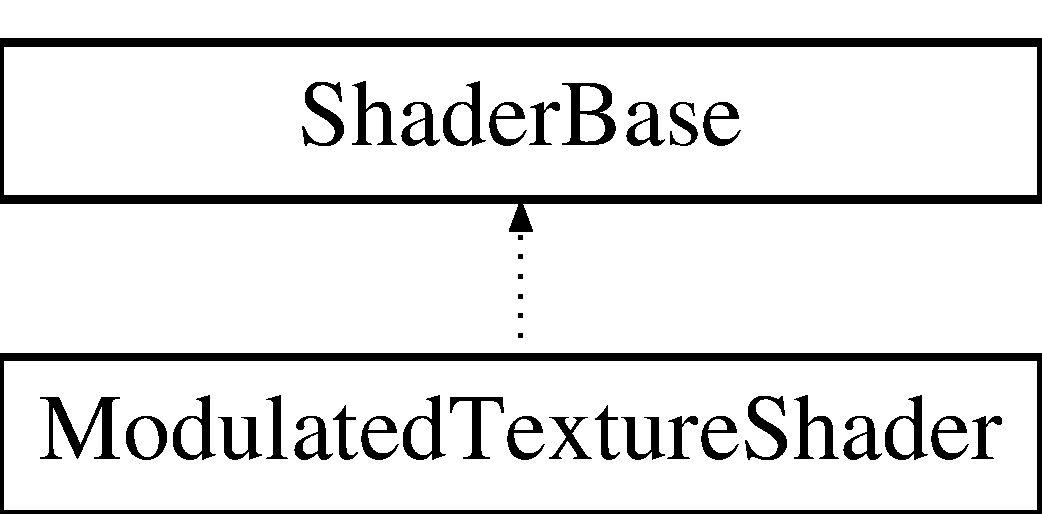
\includegraphics[height=2.000000cm]{classModulatedTextureShader}
\end{center}
\end{figure}
\subsection*{\-Public \-Types}
\begin{DoxyCompactItemize}
\item 
enum \{ {\bfseries \-V\-E\-R\-T\-E\-X\-\_\-\-I\-N\-D\-E\-X} =  0, 
{\bfseries \-T\-E\-X\-T\-U\-R\-E\-\_\-\-I\-N\-D\-E\-X} =  1, 
{\bfseries \-C\-O\-L\-O\-R\-\_\-\-I\-N\-D\-E\-X} =  2
 \}
\end{DoxyCompactItemize}
\subsection*{\-Public \-Member \-Functions}
\begin{DoxyCompactItemize}
\item 
\hypertarget{classModulatedTextureShader_a2c28abc3169683267ea6edb812fb86f1}{void {\bfseries \-Enable\-Program} (void)}\label{classModulatedTextureShader_a2c28abc3169683267ea6edb812fb86f1}

\item 
\hypertarget{classModulatedTextureShader_a4013bd45b8dfeb92c422b461aaea55fd}{void {\bfseries \-Disable\-Program} (void)}\label{classModulatedTextureShader_a4013bd45b8dfeb92c422b461aaea55fd}

\item 
\hypertarget{classModulatedTextureShader_ac31c77280c385429860dde8898bf95ea}{void {\bfseries \-Model\-View} (const glm\-::mat4 \&)}\label{classModulatedTextureShader_ac31c77280c385429860dde8898bf95ea}

\item 
\hypertarget{classModulatedTextureShader_a315d7c9ca628120da31f1b418e952888}{void {\bfseries \-Projection} (const glm\-::mat4 \&)}\label{classModulatedTextureShader_a315d7c9ca628120da31f1b418e952888}

\item 
\hypertarget{classModulatedTextureShader_a1f450015891452223c0e7d9da5c79925}{void {\bfseries \-Init} (void)}\label{classModulatedTextureShader_a1f450015891452223c0e7d9da5c79925}

\end{DoxyCompactItemize}


\-The documentation for this class was generated from the following files\-:\begin{DoxyCompactItemize}
\item 
shaders/modulatedtextureshader.\-h\item 
shaders/modulatedtextureshader.\-cpp\end{DoxyCompactItemize}

\hypertarget{classMonsters}{\section{\-Monsters \-Class \-Reference}
\label{classMonsters}\index{\-Monsters@{\-Monsters}}
}
\subsection*{\-Classes}
\begin{DoxyCompactItemize}
\item 
struct {\bfseries \-One\-Monster}
\end{DoxyCompactItemize}
\subsection*{\-Public \-Member \-Functions}
\begin{DoxyCompactItemize}
\item 
\hypertarget{classMonsters_a8d35357d16ed1b11b07a3bbee512c6c1}{void {\bfseries \-Set\-Monster} (unsigned long id, unsigned char hp, unsigned int level, signed long long x, signed long long y, signed long long z, float dir)}\label{classMonsters_a8d35357d16ed1b11b07a3bbee512c6c1}

\item 
\hypertarget{classMonsters_a1c2660b1274f680400741130571dea70}{\hyperlink{classObject}{\-Object} $\ast$ {\bfseries \-Find} (unsigned long id)}\label{classMonsters_a1c2660b1274f680400741130571dea70}

\item 
\hypertarget{classMonsters_ab7fc77e933f6c7984cb3449b080495fd}{void {\bfseries \-Render\-Monsters} (bool for\-Shadows, bool selection\-Mode, const \hyperlink{classAnimationModels}{\-Animation\-Models} $\ast$animation\-Models) const }\label{classMonsters_ab7fc77e933f6c7984cb3449b080495fd}

\item 
\hypertarget{classMonsters_a5ebd927b5c5d174833768772d39d31f2}{void {\bfseries \-Render\-Minimap} (const glm\-::mat4 \&model, \hyperlink{classHealthBar}{\-Health\-Bar} $\ast$hb) const }\label{classMonsters_a5ebd927b5c5d174833768772d39d31f2}

\item 
\hypertarget{classMonsters_a669fad1d98edf18ab53219d5476da82f}{\-One\-Monster $\ast$ {\bfseries \-Get\-Selection} (unsigned char \-R, unsigned char \-G, unsigned char \-B)}\label{classMonsters_a669fad1d98edf18ab53219d5476da82f}

\item 
\hypertarget{classMonsters_a4fcb289716127854078ba69a89079cb0}{void {\bfseries \-Cleanup} (void)}\label{classMonsters_a4fcb289716127854078ba69a89079cb0}

\item 
\hypertarget{classMonsters_acf3a50904f2bb6f36caa9499f4d88eef}{\hyperlink{classObject}{\-Object} $\ast$ {\bfseries \-Get\-Next} (\hyperlink{classObject}{\-Object} $\ast$current)}\label{classMonsters_acf3a50904f2bb6f36caa9499f4d88eef}

\end{DoxyCompactItemize}
\subsection*{\-Static \-Public \-Member \-Functions}
\begin{DoxyCompactItemize}
\item 
\hypertarget{classMonsters_a9eb8cff820a8d541ad6f623b0ae08f36}{static float {\bfseries \-Size} (unsigned int level)}\label{classMonsters_a9eb8cff820a8d541ad6f623b0ae08f36}

\end{DoxyCompactItemize}


\-The documentation for this class was generated from the following files\-:\begin{DoxyCompactItemize}
\item 
monsters.\-h\item 
monsters.\-cpp\end{DoxyCompactItemize}

\hypertarget{classMonsterShader}{\section{\-Monster\-Shader \-Class \-Reference}
\label{classMonsterShader}\index{\-Monster\-Shader@{\-Monster\-Shader}}
}
\-Inheritance diagram for \-Monster\-Shader\-:\begin{figure}[H]
\begin{center}
\leavevmode
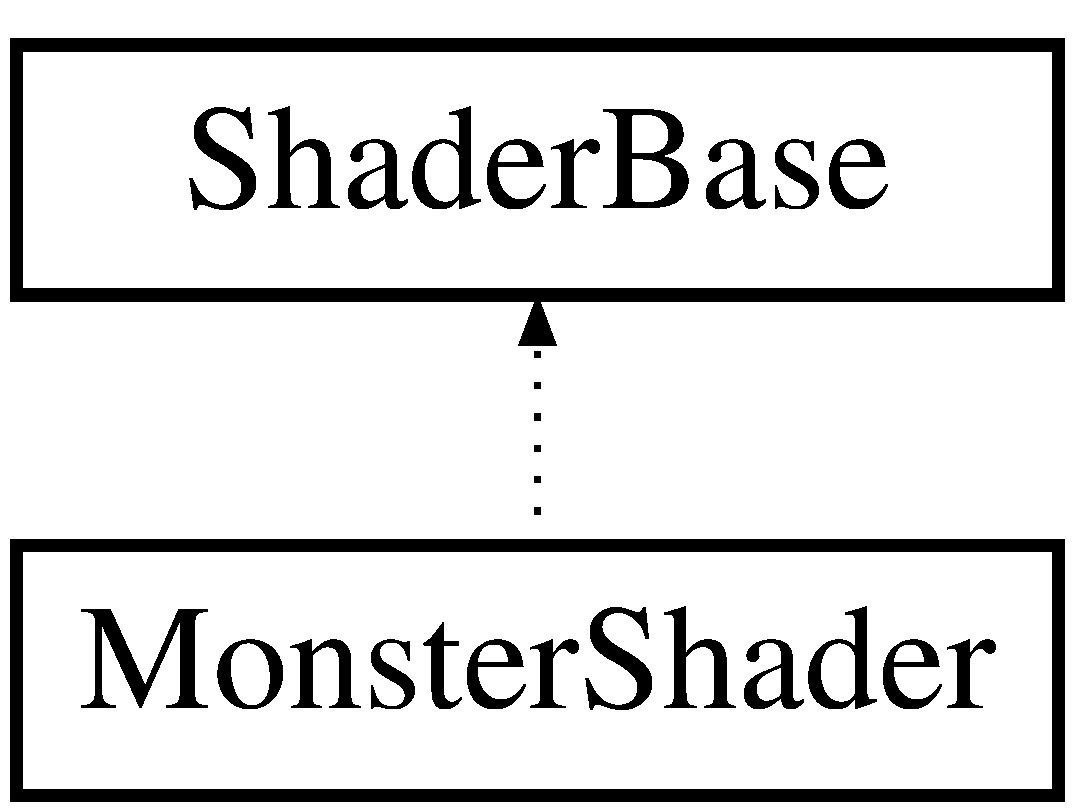
\includegraphics[height=2.000000cm]{classMonsterShader}
\end{center}
\end{figure}
\subsection*{\-Public \-Member \-Functions}
\begin{DoxyCompactItemize}
\item 
\hypertarget{classMonsterShader_a92637d67904524b2eadbb41d1e87518c}{void {\bfseries \-Enable\-Program} (void)}\label{classMonsterShader_a92637d67904524b2eadbb41d1e87518c}

\item 
\hypertarget{classMonsterShader_aa1a87c344a6bfbb4916b48e36f9923a9}{void {\bfseries \-Disable\-Program} (void)}\label{classMonsterShader_aa1a87c344a6bfbb4916b48e36f9923a9}

\item 
\hypertarget{classMonsterShader_ae5d0a0a4685f9adcec0b7026318610da}{void {\bfseries \-Model\-View} (const glm\-::mat4 \&model, const glm\-::mat4 \&view, float sun=0.\-0f, float ambient=0.\-2f)}\label{classMonsterShader_ae5d0a0a4685f9adcec0b7026318610da}

\item 
\hypertarget{classMonsterShader_aed594a6af120ccdcbf1e0343f57a56b7}{void {\bfseries \-Cycle} (unsigned char)}\label{classMonsterShader_aed594a6af120ccdcbf1e0343f57a56b7}

\item 
\hypertarget{classMonsterShader_ae2f1915756ba9070486218d48642fcec}{void {\bfseries \-Color\-Addon} (const float $\ast$)}\label{classMonsterShader_ae2f1915756ba9070486218d48642fcec}

\item 
\hypertarget{classMonsterShader_acc362d2fc6d941fd2c8d5510e8d6abee}{void {\bfseries \-Vertex\-Attrib\-Pointer} (\-G\-Lsizei stride, const \-G\-Lvoid $\ast$pointer)}\label{classMonsterShader_acc362d2fc6d941fd2c8d5510e8d6abee}

\item 
\hypertarget{classMonsterShader_a25dd31c9e686e48324f7a3071cd82969}{void {\bfseries \-Texture\-Attrib\-Pointer} (\-G\-Lsizei stride, const \-G\-Lvoid $\ast$pointer)}\label{classMonsterShader_a25dd31c9e686e48324f7a3071cd82969}

\item 
\hypertarget{classMonsterShader_ad2a46c81c37460aeeab1535253653237}{void {\bfseries \-Normal\-Attrib\-Pointer} (\-G\-Lsizei stride, const \-G\-Lvoid $\ast$offset)}\label{classMonsterShader_ad2a46c81c37460aeeab1535253653237}

\item 
\hypertarget{classMonsterShader_a69ea6ceed592808c3548826c824d3203}{void {\bfseries \-Enable\-Vertex\-Attrib\-Array} (void)}\label{classMonsterShader_a69ea6ceed592808c3548826c824d3203}

\end{DoxyCompactItemize}
\subsection*{\-Static \-Public \-Member \-Functions}
\begin{DoxyCompactItemize}
\item 
\hypertarget{classMonsterShader_abc5a799789863cfda3f646f4b5539422}{static \hyperlink{classMonsterShader}{\-Monster\-Shader} $\ast$ {\bfseries \-Make} (void)}\label{classMonsterShader_abc5a799789863cfda3f646f4b5539422}

\end{DoxyCompactItemize}
\subsection*{\-Protected \-Member \-Functions}
\begin{DoxyCompactItemize}
\item 
\hypertarget{classMonsterShader_a1ff281ab87f60b5f605c51368352c88f}{virtual void {\bfseries \-Pre\-Link\-Callback} (\-G\-Luint prg)}\label{classMonsterShader_a1ff281ab87f60b5f605c51368352c88f}

\end{DoxyCompactItemize}


\-The documentation for this class was generated from the following files\-:\begin{DoxyCompactItemize}
\item 
shaders/\-Monster\-Shader.\-h\item 
shaders/\-Monster\-Shader.\-cpp\end{DoxyCompactItemize}

\hypertarget{classMsgWindow}{\section{\-Msg\-Window \-Class \-Reference}
\label{classMsgWindow}\index{\-Msg\-Window@{\-Msg\-Window}}
}
\subsection*{\-Public \-Member \-Functions}
\begin{DoxyCompactItemize}
\item 
\hypertarget{classMsgWindow_a571ae13878e4ab906c0fd03988b79217}{void {\bfseries \-Add} (const char $\ast$fmt,...)}\label{classMsgWindow_a571ae13878e4ab906c0fd03988b79217}

\item 
\hypertarget{classMsgWindow_a31f6a0258264e36673062528d35a51cf}{void {\bfseries \-Init} (\-Rocket\-::\-Core\-::\-Element $\ast$rocket\-Element)}\label{classMsgWindow_a31f6a0258264e36673062528d35a51cf}

\item 
\hypertarget{classMsgWindow_ad2fc0ab2dd008aff2b6eb3bbfd3ead74}{void {\bfseries \-Set\-Alternate\-Position} (int x, int y, bool enable=true)}\label{classMsgWindow_ad2fc0ab2dd008aff2b6eb3bbfd3ead74}

\end{DoxyCompactItemize}


\-The documentation for this class was generated from the following files\-:\begin{DoxyCompactItemize}
\item 
msgwindow.\-h\item 
msgwindow.\-cpp\end{DoxyCompactItemize}

\hypertarget{classstd_1_1mutex}{\section{std\-:\-:mutex \-Class \-Reference}
\label{classstd_1_1mutex}\index{std\-::mutex@{std\-::mutex}}
}
\subsection*{\-Public \-Member \-Functions}
\begin{DoxyCompactItemize}
\item 
\hypertarget{classstd_1_1mutex_a487c7cb3d4f1eafd7b351dd6dcd82422}{void {\bfseries lock} (void)}\label{classstd_1_1mutex_a487c7cb3d4f1eafd7b351dd6dcd82422}

\item 
\hypertarget{classstd_1_1mutex_a13f22c85c4954c20610ab2e9023d22e8}{void {\bfseries unlock} (void)}\label{classstd_1_1mutex_a13f22c85c4954c20610ab2e9023d22e8}

\item 
\hypertarget{classstd_1_1mutex_a6d836f56c290b512299071b7e69c718c}{bool {\bfseries try\-\_\-lock} (void)}\label{classstd_1_1mutex_a6d836f56c290b512299071b7e69c718c}

\end{DoxyCompactItemize}
\subsection*{\-Public \-Attributes}
\begin{DoxyCompactItemize}
\item 
\hypertarget{classstd_1_1mutex_ad3f0ed1898da93670cc4424d5a6a3149}{pthread\-\_\-mutex\-\_\-t {\bfseries f\-Mutex}}\label{classstd_1_1mutex_ad3f0ed1898da93670cc4424d5a6a3149}

\end{DoxyCompactItemize}


\-The documentation for this class was generated from the following file\-:\begin{DoxyCompactItemize}
\item 
mythread.\-h\end{DoxyCompactItemize}

\hypertarget{classObject}{\section{\-Object \-Class \-Reference}
\label{classObject}\index{\-Object@{\-Object}}
}
\-Inheritance diagram for \-Object\-:\begin{figure}[H]
\begin{center}
\leavevmode
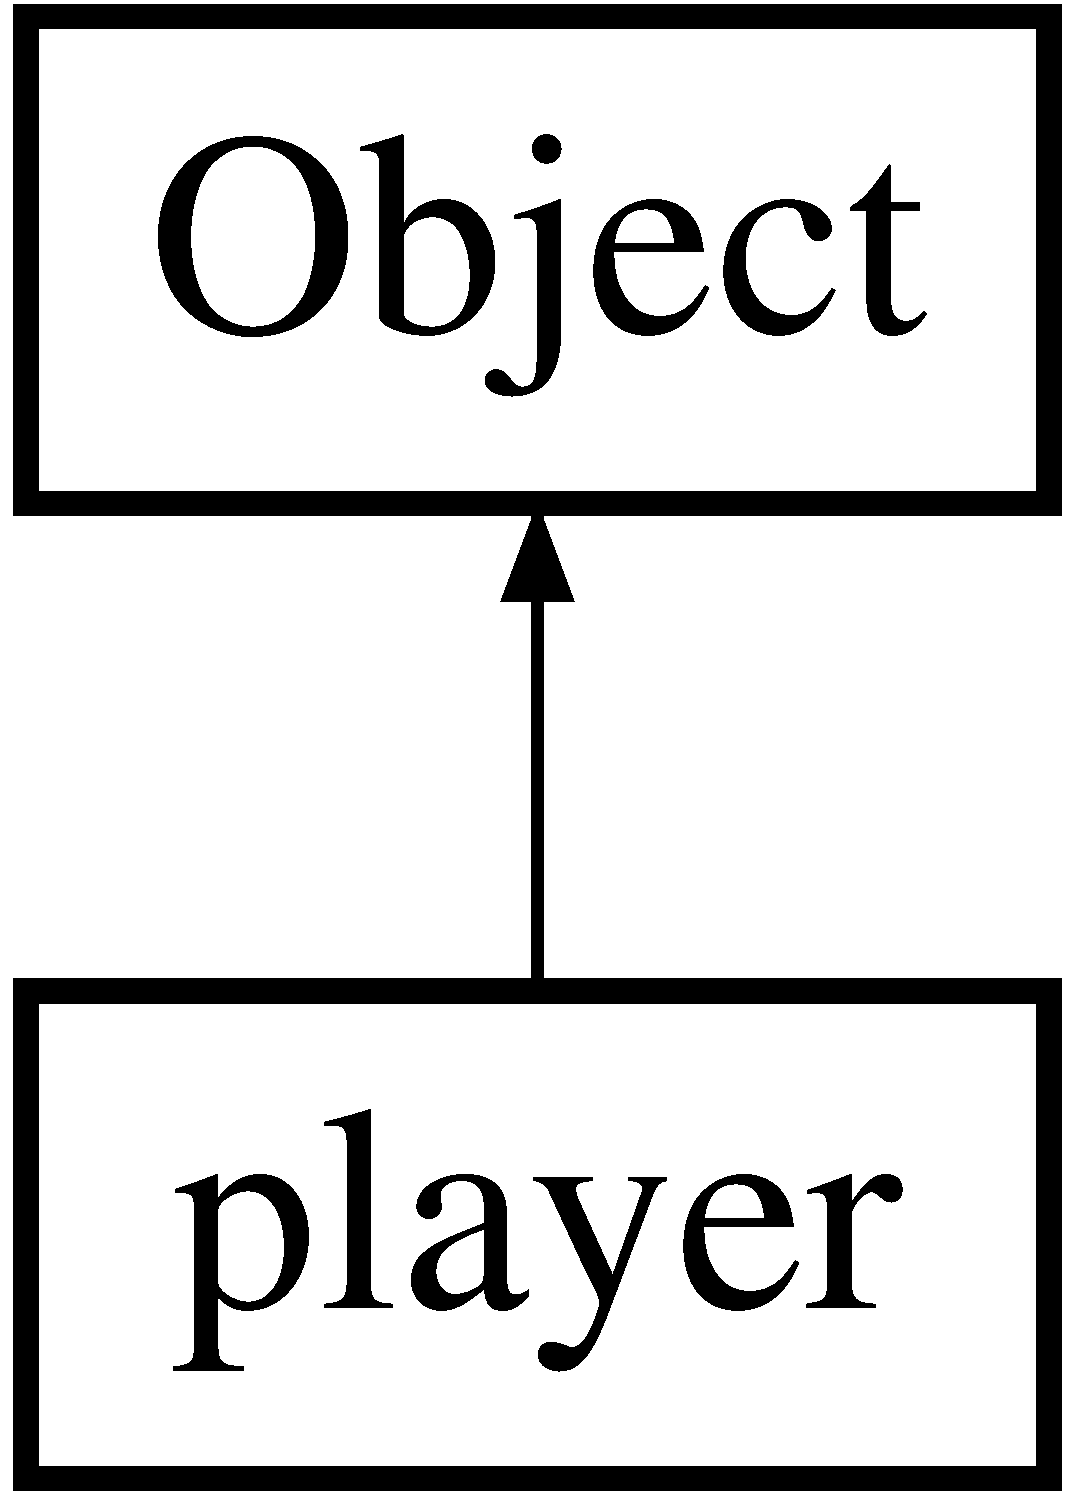
\includegraphics[height=2.000000cm]{classObject}
\end{center}
\end{figure}
\subsection*{\-Public \-Member \-Functions}
\begin{DoxyCompactItemize}
\item 
\hypertarget{classObject_a4b79c7788fc0162ca4313f64dc9de156}{virtual unsigned long {\bfseries \-Get\-Id} () const =0}\label{classObject_a4b79c7788fc0162ca4313f64dc9de156}

\item 
\hypertarget{classObject_a60afd7252818f9798afc2c65243f4a8e}{virtual int {\bfseries \-Get\-Type} () const =0}\label{classObject_a60afd7252818f9798afc2c65243f4a8e}

\item 
\hypertarget{classObject_accd0fb5338f2466a9e81b92e8f0a70a5}{virtual int {\bfseries \-Get\-Level} () const =0}\label{classObject_accd0fb5338f2466a9e81b92e8f0a70a5}

\item 
\hypertarget{classObject_a8104fa8c5faea8d84fe92a0b237a18a1}{virtual glm\-::vec3 {\bfseries \-Get\-Position} () const =0}\label{classObject_a8104fa8c5faea8d84fe92a0b237a18a1}

\item 
\hypertarget{classObject_a85e7dbfcb5f78934298e829c99b48b0f}{virtual glm\-::vec3 {\bfseries \-Get\-Selection\-Color} () const =0}\label{classObject_a85e7dbfcb5f78934298e829c99b48b0f}

\item 
\hypertarget{classObject_a768728f37f7446ea897d04b35915ad47}{virtual bool {\bfseries \-Is\-Dead} (void) const =0}\label{classObject_a768728f37f7446ea897d04b35915ad47}

\item 
\hypertarget{classObject_a6ef3dffccd332693d01ea57c322f1174}{virtual void {\bfseries \-Render\-Health\-Bar} (\hyperlink{classHealthBar}{\-Health\-Bar} $\ast$, float angle) const =0}\label{classObject_a6ef3dffccd332693d01ea57c322f1174}

\item 
\hypertarget{classObject_a65c6fc1c9d3b1b6ef2a173c69fcc39a1}{virtual bool {\bfseries \-In\-Game} (void) const =0}\label{classObject_a65c6fc1c9d3b1b6ef2a173c69fcc39a1}

\end{DoxyCompactItemize}


\-The documentation for this class was generated from the following file\-:\begin{DoxyCompactItemize}
\item 
object.\-h\end{DoxyCompactItemize}

\hypertarget{structInventory_1_1ObjectMap}{\section{\-Inventory\-:\-:\-Object\-Map \-Struct \-Reference}
\label{structInventory_1_1ObjectMap}\index{\-Inventory\-::\-Object\-Map@{\-Inventory\-::\-Object\-Map}}
}
\subsection*{\-Public \-Attributes}
\begin{DoxyCompactItemize}
\item 
\hypertarget{structInventory_1_1ObjectMap_ada02bed6b7729e7fbd7981b3bb5cc341}{const char $\ast$ {\bfseries descr}}\label{structInventory_1_1ObjectMap_ada02bed6b7729e7fbd7981b3bb5cc341}

\item 
\hypertarget{structInventory_1_1ObjectMap_af7ee9d2417589882df0421b68d3a577c}{const char $\ast$ {\bfseries code}}\label{structInventory_1_1ObjectMap_af7ee9d2417589882df0421b68d3a577c}

\item 
\hypertarget{structInventory_1_1ObjectMap_a6641e52f2a3552b9006c8a7338d9957a}{\-Sound\-Control\-::\-Sound {\bfseries song}}\label{structInventory_1_1ObjectMap_a6641e52f2a3552b9006c8a7338d9957a}

\item 
\hypertarget{structInventory_1_1ObjectMap_a505aecaea9c664fbe025ad9504151913}{float {\bfseries x\-Offset}}\label{structInventory_1_1ObjectMap_a505aecaea9c664fbe025ad9504151913}

\item 
\hypertarget{structInventory_1_1ObjectMap_ab3d1634e4a88c82474681aa624f50cab}{float {\bfseries y\-Offset}}\label{structInventory_1_1ObjectMap_ab3d1634e4a88c82474681aa624f50cab}

\item 
\hypertarget{structInventory_1_1ObjectMap_a945bc8d8cdcbc4dba9c45ea195504c2a}{bool {\bfseries depend\-On\-Level}}\label{structInventory_1_1ObjectMap_a945bc8d8cdcbc4dba9c45ea195504c2a}

\item 
\hypertarget{structInventory_1_1ObjectMap_aece3298428d71891db0060023100d35e}{\-Inventory\-Category {\bfseries category}}\label{structInventory_1_1ObjectMap_aece3298428d71891db0060023100d35e}

\end{DoxyCompactItemize}


\-The documentation for this struct was generated from the following file\-:\begin{DoxyCompactItemize}
\item 
\-Inventory.\-h\end{DoxyCompactItemize}

\hypertarget{classOptions}{\section{\-Options \-Class \-Reference}
\label{classOptions}\index{\-Options@{\-Options}}
}
\subsection*{\-Public \-Member \-Functions}
\begin{DoxyCompactItemize}
\item 
\hypertarget{classOptions_ad3b1d757066830755ef9f6aa5e385fa7}{void {\bfseries \-Init} (const std\-::string \&file\-Name)}\label{classOptions_ad3b1d757066830755ef9f6aa5e385fa7}

\item 
\hypertarget{classOptions_aab1c845d114dec4f25c2c51b73d3da42}{void {\bfseries \-List\-Graphic\-Modes} (\-Rocket\-::\-Controls\-::\-Element\-Form\-Control\-Select $\ast$) const }\label{classOptions_aab1c845d114dec4f25c2c51b73d3da42}

\item 
\hypertarget{classOptions_a4f217bfbf7410778c79b19dedc9eb9ec}{void {\bfseries \-Set\-Graphics\-Mode} (int)}\label{classOptions_a4f217bfbf7410778c79b19dedc9eb9ec}

\item 
\hypertarget{classOptions_af3c3360d7cb6f9ce9949ce026ec59413}{bool {\bfseries \-Parse\-One\-Option} (const string \&key, const string \&arg)}\label{classOptions_af3c3360d7cb6f9ce9949ce026ec59413}

\item 
\hypertarget{classOptions_a804a3834fa4f3dcca0506b04a6797a52}{void {\bfseries \-Save} (void)}\label{classOptions_a804a3834fa4f3dcca0506b04a6797a52}

\item 
\hypertarget{classOptions_affdf37b165ac81501a63aee112946f1c}{void {\bfseries \-Update\-Performance} (int perf)}\label{classOptions_affdf37b165ac81501a63aee112946f1c}

\end{DoxyCompactItemize}
\subsection*{\-Public \-Attributes}
\begin{DoxyCompactItemize}
\item 
\hypertarget{classOptions_ae6bf58ccb780aef459152e546c1511e5}{std\-::string {\bfseries f\-Email}}\label{classOptions_ae6bf58ccb780aef459152e546c1511e5}

\item 
\hypertarget{classOptions_aaaac4bb89fa308b3b74d880d3bc0277c}{std\-::string {\bfseries f\-License\-Key}}\label{classOptions_aaaac4bb89fa308b3b74d880d3bc0277c}

\item 
\hypertarget{classOptions_a70b945ff172979f0005b522c55f66034}{float {\bfseries f\-Viewing\-Distance}}\label{classOptions_a70b945ff172979f0005b522c55f66034}

\item 
\hypertarget{classOptions_a9b573114db66f1bbf035ff66a37cccc6}{float {\bfseries f\-Camera\-Distance}}\label{classOptions_a9b573114db66f1bbf035ff66a37cccc6}

\item 
\hypertarget{classOptions_a848ea5ec020a8c64ea311f7a4bfd232b}{float {\bfseries f\-White\-Point}}\label{classOptions_a848ea5ec020a8c64ea311f7a4bfd232b}

\item 
\hypertarget{classOptions_a904f271d332054dd94662c0a9bab5e9a}{float {\bfseries f\-Exposure}}\label{classOptions_a904f271d332054dd94662c0a9bab5e9a}

\item 
\hypertarget{classOptions_a469f04eb19ead120ea8adc270154504d}{int {\bfseries f\-Window\-Width}}\label{classOptions_a469f04eb19ead120ea8adc270154504d}

\item 
\hypertarget{classOptions_a9ba8f9f07c457ab29d171e0458421ecc}{int {\bfseries f\-Window\-Height}}\label{classOptions_a9ba8f9f07c457ab29d171e0458421ecc}

\item 
\hypertarget{classOptions_aab8c157677e2c5b5677b99022ea1066a}{int {\bfseries f\-Font\-Size}}\label{classOptions_aab8c157677e2c5b5677b99022ea1066a}

\item 
\hypertarget{classOptions_a084d95230886875d011f3aa271c81504}{int {\bfseries f\-Msg\-Win\-Transparency}}\label{classOptions_a084d95230886875d011f3aa271c81504}

\item 
\hypertarget{classOptions_a9282fcff6e3f3178fc88912c0d0148e1}{int {\bfseries f\-Music\-Volume}}\label{classOptions_a9282fcff6e3f3178fc88912c0d0148e1}

\item 
\hypertarget{classOptions_ae88516146d2be09edd95b03ec94a2fb5}{int {\bfseries f\-Music\-On}}\label{classOptions_ae88516146d2be09edd95b03ec94a2fb5}

\item 
\hypertarget{classOptions_aab7a79a78de3447f71038671264b3a38}{int {\bfseries f\-Sound\-Fx\-Volume}}\label{classOptions_aab7a79a78de3447f71038671264b3a38}

\item 
\hypertarget{classOptions_aabdcc86eaa69c83981adf710deeba84d}{int {\bfseries f\-Enable\-Testbutton}}\label{classOptions_aabdcc86eaa69c83981adf710deeba84d}

\item 
\hypertarget{classOptions_af11cb04eb12eb3ff63298e986887c10e}{int {\bfseries f\-Performance}}\label{classOptions_af11cb04eb12eb3ff63298e986887c10e}

\item 
\hypertarget{classOptions_a11a8c1acd279d9ec20a82cbe7c874a1c}{int {\bfseries f\-New\-Performance}}\label{classOptions_a11a8c1acd279d9ec20a82cbe7c874a1c}

\item 
\hypertarget{classOptions_ad0185e6c6770c5ca407f9aab57b414c7}{int {\bfseries f\-Max\-Lamps}}\label{classOptions_ad0185e6c6770c5ca407f9aab57b414c7}

\item 
\hypertarget{classOptions_a9b6c91fdd2595307c54e209f28c327ee}{int {\bfseries f\-Max\-Shadows}}\label{classOptions_a9b6c91fdd2595307c54e209f28c327ee}

\item 
\hypertarget{classOptions_a2ff58fff400e338b9eb1594799282093}{int {\bfseries f\-Max\-Fog}}\label{classOptions_a2ff58fff400e338b9eb1594799282093}

\item 
\hypertarget{classOptions_addd319968aa8ac15dc69ea2c0779896c}{int {\bfseries f\-Full\-Screen}}\label{classOptions_addd319968aa8ac15dc69ea2c0779896c}

\item 
\hypertarget{classOptions_a360a2479f3679ef48e31b530f845580c}{int {\bfseries f\-Ambient\-Light}}\label{classOptions_a360a2479f3679ef48e31b530f845580c}

\item 
\hypertarget{classOptions_a4edc6f1b294298f23ed621e94b501e9e}{int {\bfseries f\-Smooth\-Terrain}}\label{classOptions_a4edc6f1b294298f23ed621e94b501e9e}

\item 
\hypertarget{classOptions_ace531d3b4286e382b66b1045480674f2}{int {\bfseries f\-Merge\-Normals}}\label{classOptions_ace531d3b4286e382b66b1045480674f2}

\item 
\hypertarget{classOptions_a308754b4e337539c7c147b718cb47593}{int {\bfseries f\-Add\-Noise}}\label{classOptions_a308754b4e337539c7c147b718cb47593}

\item 
\hypertarget{classOptions_a35f94bd76d6e571d43f9c48cbeaab2c6}{int {\bfseries f\-Dynamic\-Shadows}}\label{classOptions_a35f94bd76d6e571d43f9c48cbeaab2c6}

\item 
\hypertarget{classOptions_a211a7de4b1061929d75fe1bb649545cc}{int {\bfseries f\-Static\-Shadows}}\label{classOptions_a211a7de4b1061929d75fe1bb649545cc}

\item 
\hypertarget{classOptions_a99152b2f23a6c0fd27761d894cf56bc4}{int {\bfseries f\-Anisotropic\-Filtering}}\label{classOptions_a99152b2f23a6c0fd27761d894cf56bc4}

\item 
\hypertarget{classOptions_ac24623e567431c087f1e775bf5d9d4cd}{int {\bfseries f\-V\-S\-Y\-N\-C}}\label{classOptions_ac24623e567431c087f1e775bf5d9d4cd}

\item 
\hypertarget{classOptions_a6da4ec772d609128c8c7af337a7e0396}{unsigned {\bfseries f\-Num\-Threads}}\label{classOptions_a6da4ec772d609128c8c7af337a7e0396}

\item 
\hypertarget{classOptions_a87774797fde0e64291dd316852067c5b}{signed long long {\bfseries f\-Player\-X}}\label{classOptions_a87774797fde0e64291dd316852067c5b}

\item 
\hypertarget{classOptions_a61a8b1b35891bf452da9dd67b7775825}{signed long long {\bfseries f\-Player\-Y}}\label{classOptions_a61a8b1b35891bf452da9dd67b7775825}

\item 
\hypertarget{classOptions_ac4df8a7ca3a4726c790d5867dcd83166}{signed long long {\bfseries f\-Player\-Z}}\label{classOptions_ac4df8a7ca3a4726c790d5867dcd83166}

\end{DoxyCompactItemize}
\subsection*{\-Static \-Public \-Attributes}
\begin{DoxyCompactItemize}
\item 
\hypertarget{classOptions_a31107388eb391548487b39003112a8ec}{static \hyperlink{classOptions}{\-Options} {\bfseries sf\-Save}}\label{classOptions_a31107388eb391548487b39003112a8ec}

\end{DoxyCompactItemize}


\-The documentation for this class was generated from the following files\-:\begin{DoxyCompactItemize}
\item 
\-Options.\-h\item 
\-Options.\-cpp\end{DoxyCompactItemize}

\hypertarget{classOtherPlayers}{\section{\-Other\-Players \-Class \-Reference}
\label{classOtherPlayers}\index{\-Other\-Players@{\-Other\-Players}}
}
\subsection*{\-Classes}
\begin{DoxyCompactItemize}
\item 
struct {\bfseries \-One\-Other\-Player}
\end{DoxyCompactItemize}
\subsection*{\-Public \-Member \-Functions}
\begin{DoxyCompactItemize}
\item 
\hypertarget{classOtherPlayers_aaf13dca14e26b815d99f4a8906aa7913}{void {\bfseries \-Cleanup} (void)}\label{classOtherPlayers_aaf13dca14e26b815d99f4a8906aa7913}

\item 
\hypertarget{classOtherPlayers_a5478a24371893c3cf31486932fe80933}{void {\bfseries \-Set\-Player} (unsigned long id, unsigned char hp, unsigned int level, signed long long x, signed long long y, signed long long z, float dir)}\label{classOtherPlayers_a5478a24371893c3cf31486932fe80933}

\item 
\hypertarget{classOtherPlayers_a17e3724b9eafb5d2458ab7c37cf03787}{void {\bfseries \-Set\-Player\-Name} (unsigned long uid, const char $\ast$name, int n, int admin\-Level)}\label{classOtherPlayers_a17e3724b9eafb5d2458ab7c37cf03787}

\item 
\hypertarget{classOtherPlayers_a48df458b7ea6db73624a059b912781d1}{void {\bfseries \-Render\-Players} (\hyperlink{classAnimationShader}{\-Animation\-Shader} $\ast$anim\-Shader, bool selection\-Mode) const }\label{classOtherPlayers_a48df458b7ea6db73624a059b912781d1}

\item 
\hypertarget{classOtherPlayers_a2ddc2ab1873fa5e7fb31f5b4dc0dfae0}{void {\bfseries \-Render\-Player\-Stats} (\hyperlink{classHealthBar}{\-Health\-Bar} $\ast$hb, float angle) const }\label{classOtherPlayers_a2ddc2ab1873fa5e7fb31f5b4dc0dfae0}

\item 
\hypertarget{classOtherPlayers_a3aac7bedea552c3c7affdf373b9f20fa}{\-One\-Other\-Player $\ast$ {\bfseries \-Get\-Selection} (unsigned char \-R, unsigned char \-G, unsigned char \-B)}\label{classOtherPlayers_a3aac7bedea552c3c7affdf373b9f20fa}

\item 
\hypertarget{classOtherPlayers_ae5305ae3e8be76f8bf888d811fb16e70}{void {\bfseries \-Render\-Minimap} (const glm\-::mat4 \&mini\-Map, \hyperlink{classHealthBar}{\-Health\-Bar} $\ast$hb) const }\label{classOtherPlayers_ae5305ae3e8be76f8bf888d811fb16e70}

\end{DoxyCompactItemize}


\-The documentation for this class was generated from the following files\-:\begin{DoxyCompactItemize}
\item 
otherplayers.\-h\item 
otherplayers.\-cpp\end{DoxyCompactItemize}

\hypertarget{unionPickingData}{\section{\-Picking\-Data \-Union \-Reference}
\label{unionPickingData}\index{\-Picking\-Data@{\-Picking\-Data}}
}
\subsection*{\-Public \-Attributes}
\begin{DoxyCompactItemize}
\item 
\hypertarget{unionPickingData_ae27efdf8fcc6b6b960ac962a4f233b3c}{unsigned char {\bfseries rgb} \mbox{[}3\mbox{]}}\label{unionPickingData_ae27efdf8fcc6b6b960ac962a4f233b3c}

\item 
\hypertarget{unionPickingData_ad4d5c088048ccd992f4a07d60fc48e7f}{\begin{tabbing}
xx\=xx\=xx\=xx\=xx\=xx\=xx\=xx\=xx\=\kill
struct \{\\
\>unsigned int {\bfseries x}:5\\
\>unsigned int {\bfseries y}:5\\
\>unsigned int {\bfseries z}:5\\
\>unsigned int {\bfseries facing}:3\\
\>unsigned int {\bfseries dx}:2\\
\>unsigned int {\bfseries dy}:2\\
\>unsigned int {\bfseries dz}:2\\
\} {\bfseries bitmap}}\label{unionPickingData_ad4d5c088048ccd992f4a07d60fc48e7f}
\\

\end{tabbing}\end{DoxyCompactItemize}


\-The documentation for this union was generated from the following file\-:\begin{DoxyCompactItemize}
\item 
primitives.\-h\end{DoxyCompactItemize}

\hypertarget{classplayer}{\section{player \-Class \-Reference}
\label{classplayer}\index{player@{player}}
}
\-Inheritance diagram for player\-:\begin{figure}[H]
\begin{center}
\leavevmode
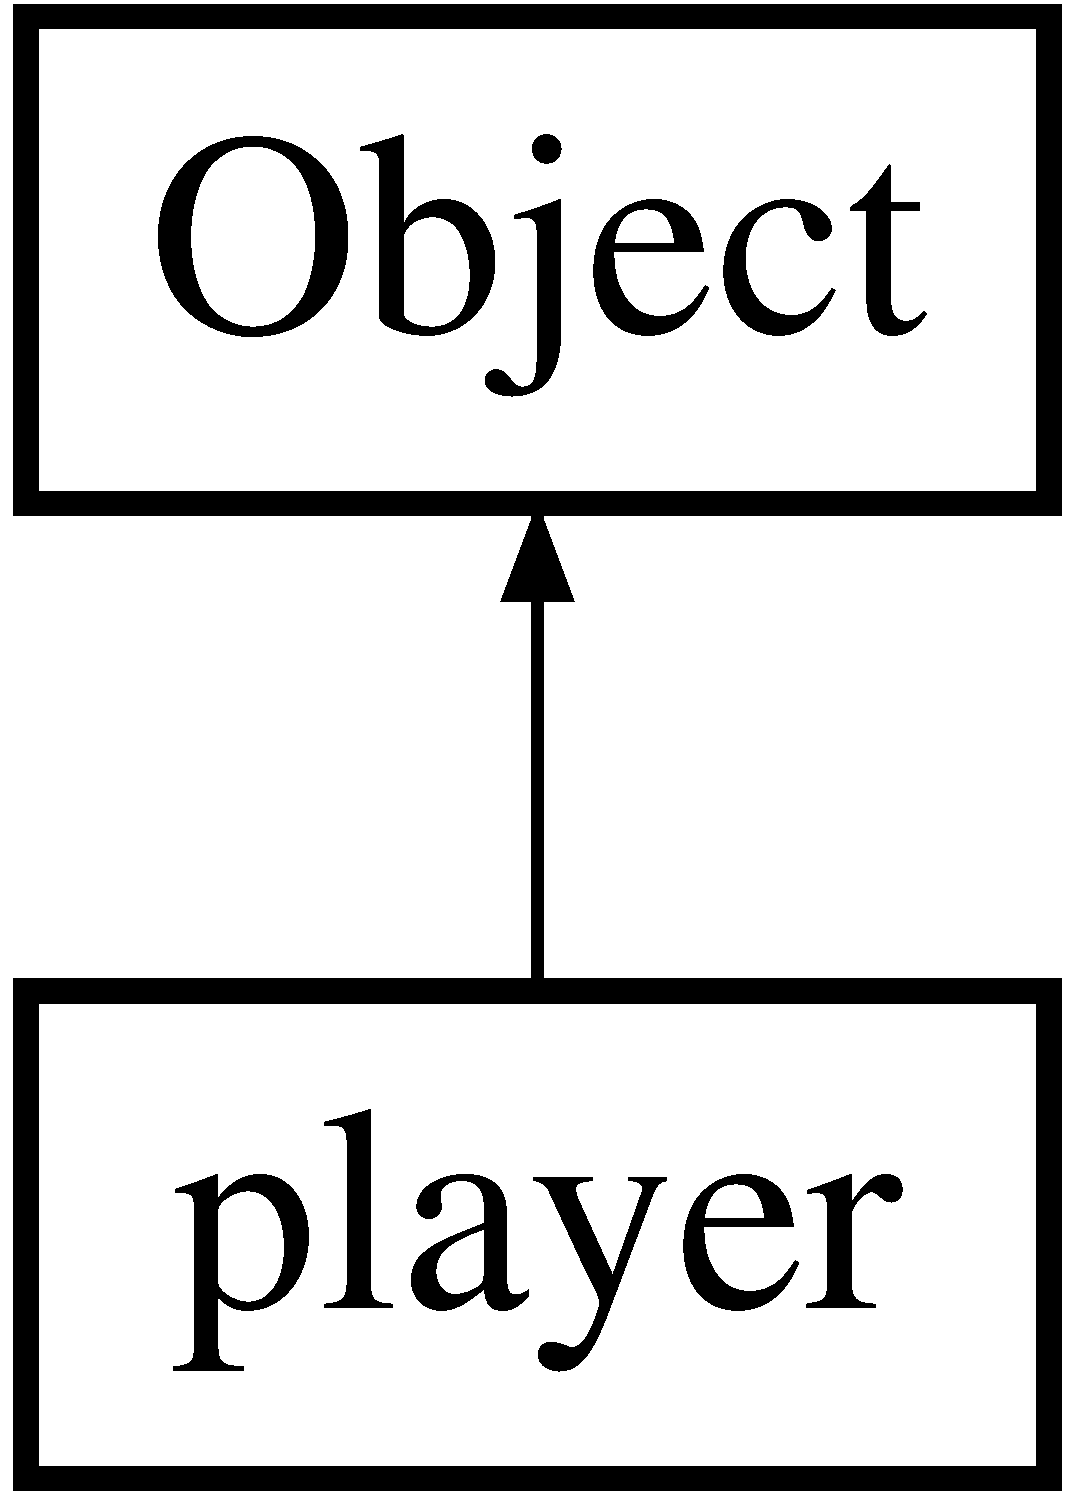
\includegraphics[height=2.000000cm]{classplayer}
\end{center}
\end{figure}
\subsection*{\-Public \-Member \-Functions}
\begin{DoxyCompactItemize}
\item 
\hypertarget{classplayer_a358865db54f32055a750de403f28d945}{void {\bfseries \-Get\-Chunk\-Coord} (\hyperlink{structChunkCoord}{\-Chunk\-Coord} $\ast$) const }\label{classplayer_a358865db54f32055a750de403f28d945}

\item 
\hypertarget{classplayer_a554d91934bef7aefa2794d1a851a6e0d}{glm\-::vec3 {\bfseries \-Get\-Offset\-To\-Chunk} (void) const }\label{classplayer_a554d91934bef7aefa2794d1a851a6e0d}

\item 
\hypertarget{classplayer_a67fecc1b289a8690966372d1269b21ec}{bool {\bfseries \-In\-Fight} (void) const }\label{classplayer_a67fecc1b289a8690966372d1269b21ec}

\item 
\hypertarget{classplayer_a5d2a8869c20a0ebaeba6dd851e80663e}{void {\bfseries \-Draw} (\hyperlink{classAnimationShader}{\-Animation\-Shader} $\ast$anim\-Shader, \hyperlink{classStageOneShader}{\-Stage\-One\-Shader} $\ast$static\-Shader, bool torch, const \hyperlink{classAnimationModels}{\-Animation\-Models} $\ast$animation\-Models)}\label{classplayer_a5d2a8869c20a0ebaeba6dd851e80663e}

\item 
\hypertarget{classplayer_a960c789b7a8260d5ed03285b580429fb}{virtual unsigned long {\bfseries \-Get\-Id} () const }\label{classplayer_a960c789b7a8260d5ed03285b580429fb}

\item 
\hypertarget{classplayer_ae90dd08c6d30e101c04e3936b0a4c888}{virtual int {\bfseries \-Get\-Type} () const }\label{classplayer_ae90dd08c6d30e101c04e3936b0a4c888}

\item 
\hypertarget{classplayer_af7e76c982912a113ef3c6c55ae488e19}{virtual int {\bfseries \-Get\-Level} () const }\label{classplayer_af7e76c982912a113ef3c6c55ae488e19}

\item 
\hypertarget{classplayer_aa5b3305c0398ed45e66077ae002842e4}{virtual glm\-::vec3 {\bfseries \-Get\-Position} () const }\label{classplayer_aa5b3305c0398ed45e66077ae002842e4}

\item 
\hypertarget{classplayer_a88f97c3a1e051fcca503296f548dcf0c}{virtual glm\-::vec3 {\bfseries \-Get\-Selection\-Color} () const }\label{classplayer_a88f97c3a1e051fcca503296f548dcf0c}

\item 
\hypertarget{classplayer_a1862f089ce1d4b1ae0c27cbc89f3d62e}{virtual bool {\bfseries \-Is\-Dead} (void) const }\label{classplayer_a1862f089ce1d4b1ae0c27cbc89f3d62e}

\item 
\hypertarget{classplayer_adcdc22d5c55604633367b67534fdb2b5}{virtual void {\bfseries \-Render\-Health\-Bar} (\hyperlink{classHealthBar}{\-Health\-Bar} $\ast$, float angle) const }\label{classplayer_adcdc22d5c55604633367b67534fdb2b5}

\item 
\hypertarget{classplayer_a0fb5b7037a769f799f8676132a8734a3}{virtual bool {\bfseries \-In\-Game} (void) const }\label{classplayer_a0fb5b7037a769f799f8676132a8734a3}

\item 
\hypertarget{classplayer_a6b27f5740d57047856427bdd22b8a1eb}{bool {\bfseries \-Below\-Ground} (void) const }\label{classplayer_a6b27f5740d57047856427bdd22b8a1eb}

\item 
\hypertarget{classplayer_a397e823a7b348d77cd41a43d7855d994}{void {\bfseries \-Set\-Position} (signed long long newx, signed long long newy, signed long long newz)}\label{classplayer_a397e823a7b348d77cd41a43d7855d994}

\item 
\hypertarget{classplayer_a55d31c3abd14980e93074bf3c8051315}{void {\bfseries \-Update\-Position\-Smooth} (void)}\label{classplayer_a55d31c3abd14980e93074bf3c8051315}

\item 
\hypertarget{classplayer_a3ca3f0997636944be261bfa5120041ea}{bool {\bfseries \-Known\-Position} () const }\label{classplayer_a3ca3f0997636944be261bfa5120041ea}

\item 
\hypertarget{classplayer_a2e6f48ac250986cdcde88f949a05c2db}{bool {\bfseries \-Player\-Is\-Moving} (void) const }\label{classplayer_a2e6f48ac250986cdcde88f949a05c2db}

\end{DoxyCompactItemize}
\subsection*{\-Public \-Attributes}
\begin{DoxyCompactItemize}
\item 
\hypertarget{classplayer_a88d55d5faf07fb608bb3c316f031f1d1}{signed long long {\bfseries x}}\label{classplayer_a88d55d5faf07fb608bb3c316f031f1d1}

\item 
\hypertarget{classplayer_ad18a0b682ce1bae4fd586013cc5aeae9}{signed long long {\bfseries y}}\label{classplayer_ad18a0b682ce1bae4fd586013cc5aeae9}

\item 
\hypertarget{classplayer_ac305917b2e1f3f3e4dfb3c7306cb3018}{signed long long {\bfseries z}}\label{classplayer_ac305917b2e1f3f3e4dfb3c7306cb3018}

\item 
\hypertarget{classplayer_a8d2676e09ea9e9fc3ce5d7e2e37a1556}{float {\bfseries f\-Angle\-Hor}}\label{classplayer_a8d2676e09ea9e9fc3ce5d7e2e37a1556}

\item 
\hypertarget{classplayer_a322c447d7aac2a0506adda0f3cac9b00}{float {\bfseries f\-Angle\-Vert}}\label{classplayer_a322c447d7aac2a0506adda0f3cac9b00}

\item 
\hypertarget{classplayer_a1bf306a353825eb0e343f7335a0f5edc}{bool {\bfseries login\-Ok}}\label{classplayer_a1bf306a353825eb0e343f7335a0f5edc}

\item 
\hypertarget{classplayer_ac9f8766b16181f113e7fab1730f4af10}{bool {\bfseries f\-Stats\-Available}}\label{classplayer_ac9f8766b16181f113e7fab1730f4af10}

\item 
\hypertarget{classplayer_a971af9ed2ec704d09f1a49a2acf4e2f6}{float {\bfseries f\-Hp}}\label{classplayer_a971af9ed2ec704d09f1a49a2acf4e2f6}

\item 
\hypertarget{classplayer_a5b52487b3a17471430a0c5a8c9c3c5bc}{float {\bfseries f\-Previous\-Hp}}\label{classplayer_a5b52487b3a17471430a0c5a8c9c3c5bc}

\item 
\hypertarget{classplayer_a7f4a2912e06b8b84298e2499bb1ed540}{float {\bfseries f\-Exp}}\label{classplayer_a7f4a2912e06b8b84298e2499bb1ed540}

\item 
\hypertarget{classplayer_a6b167313d7b4b55c29ad6e68062bbe46}{float {\bfseries f\-Mana}}\label{classplayer_a6b167313d7b4b55c29ad6e68062bbe46}

\item 
\hypertarget{classplayer_aaa06e1028540c458c3f4f2fe6dcf1fa3}{unsigned long {\bfseries f\-Level}}\label{classplayer_aaa06e1028540c458c3f4f2fe6dcf1fa3}

\item 
\hypertarget{classplayer_a5241983acfa028407a099474e34e6abf}{unsigned char {\bfseries f\-Admin}}\label{classplayer_a5241983acfa028407a099474e34e6abf}

\item 
\hypertarget{classplayer_a9f8bf5485ace587327421f1baa667789}{unsigned long {\bfseries f\-Uid}}\label{classplayer_a9f8bf5485ace587327421f1baa667789}

\item 
\hypertarget{classplayer_acb3b632457f8051402696878577d49e0}{unsigned long {\bfseries f\-Flags}}\label{classplayer_acb3b632457f8051402696878577d49e0}

\item 
\hypertarget{classplayer_a374b721c5a66db6b7e9290a031094743}{unsigned char {\bfseries f\-Weapon\-Type}}\label{classplayer_a374b721c5a66db6b7e9290a031094743}

\item 
\hypertarget{classplayer_a23607d669aae25fc6f88081aded49383}{unsigned long {\bfseries f\-Weapon\-Level}}\label{classplayer_a23607d669aae25fc6f88081aded49383}

\item 
\hypertarget{classplayer_a56013e3d22640531c102419b8a845be0}{unsigned char {\bfseries f\-Armor\-Type}}\label{classplayer_a56013e3d22640531c102419b8a845be0}

\item 
\hypertarget{classplayer_a33fa80a6d4f45c9c80bc4bd490de13d1}{unsigned long {\bfseries f\-Armor\-Level}}\label{classplayer_a33fa80a6d4f45c9c80bc4bd490de13d1}

\item 
\hypertarget{classplayer_abc76c3d2c7d81e7bcf1dc8e41b4fca13}{unsigned char {\bfseries f\-Helmet\-Type}}\label{classplayer_abc76c3d2c7d81e7bcf1dc8e41b4fca13}

\item 
\hypertarget{classplayer_a0b378b51a70fc42ecfd3b9e5ba4d8d50}{unsigned long {\bfseries f\-Helmet\-Level}}\label{classplayer_a0b378b51a70fc42ecfd3b9e5ba4d8d50}

\end{DoxyCompactItemize}


\-The documentation for this class was generated from the following files\-:\begin{DoxyCompactItemize}
\item 
player.\-h\item 
player.\-cpp\end{DoxyCompactItemize}

\hypertarget{classQuad}{\section{\-Quad \-Class \-Reference}
\label{classQuad}\index{\-Quad@{\-Quad}}
}


\-A very minimal shape, drawing a quad from 0 to 1 in x and y. \-A simple quad drawn using \-V\-A\-O and \-V\-B\-O.  




{\ttfamily \#include $<$quad.\-h$>$}

\subsection*{\-Public \-Member \-Functions}
\begin{DoxyCompactItemize}
\item 
\hypertarget{classQuad_ac9fd55b0f273d9829f7991c3fdfc80ee}{void \hyperlink{classQuad_ac9fd55b0f273d9829f7991c3fdfc80ee}{\-Draw} (void)}\label{classQuad_ac9fd55b0f273d9829f7991c3fdfc80ee}

\begin{DoxyCompactList}\small\item\em \-The draw routine. \end{DoxyCompactList}\end{DoxyCompactItemize}


\subsection{\-Detailed \-Description}
\-A very minimal shape, drawing a quad from 0 to 1 in x and y. \-A simple quad drawn using \-V\-A\-O and \-V\-B\-O. 

\begin{DoxyRefDesc}{\-Todo}
\item[\hyperlink{todo__todo000005}{\-Todo}]\-Why not inherit from \hyperlink{classShaderBase}{\-Shader\-Base}? \end{DoxyRefDesc}


\-The documentation for this class was generated from the following files\-:\begin{DoxyCompactItemize}
\item 
shapes/quad.\-h\item 
shapes/quad.\-cpp\end{DoxyCompactItemize}

\hypertarget{classQuadStage1}{\section{\-Quad\-Stage1 \-Class \-Reference}
\label{classQuadStage1}\index{\-Quad\-Stage1@{\-Quad\-Stage1}}
}
\subsection*{\-Public \-Member \-Functions}
\begin{DoxyCompactItemize}
\item 
\hypertarget{classQuadStage1_aa3c6d9b8e67c105549ff641426e14841}{void {\bfseries \-Init} (void)}\label{classQuadStage1_aa3c6d9b8e67c105549ff641426e14841}

\item 
\hypertarget{classQuadStage1_a0708389164a78bfed94357c82fdbaffb}{void {\bfseries \-Draw\-Double\-Side} (void) const }\label{classQuadStage1_a0708389164a78bfed94357c82fdbaffb}

\item 
\hypertarget{classQuadStage1_a3f2bc17e1d89255560cb603a4251a6ee}{void {\bfseries \-Draw\-Single\-Side} (void) const }\label{classQuadStage1_a3f2bc17e1d89255560cb603a4251a6ee}

\item 
\hypertarget{classQuadStage1_aff9fa9ff12d1f40ee535b9f68b02e3f2}{void {\bfseries \-Draw\-Lines} (void) const }\label{classQuadStage1_aff9fa9ff12d1f40ee535b9f68b02e3f2}

\end{DoxyCompactItemize}


\-The documentation for this class was generated from the following files\-:\begin{DoxyCompactItemize}
\item 
shapes/quadstage1.\-h\item 
shapes/quadstage1.\-cpp\end{DoxyCompactItemize}

\hypertarget{classRenderControl}{\section{\-Render\-Control \-Class \-Reference}
\label{classRenderControl}\index{\-Render\-Control@{\-Render\-Control}}
}
\subsection*{\-Public \-Member \-Functions}
\begin{DoxyCompactItemize}
\item 
\hypertarget{classRenderControl_a27ff96bb3b07efb33bdd11aa24b4f4b3}{void {\bfseries \-Resize} (\-G\-Lsizei width, \-G\-Lsizei height)}\label{classRenderControl_a27ff96bb3b07efb33bdd11aa24b4f4b3}

\item 
\hypertarget{classRenderControl_a0107433760a1f931231d6d4396130c01}{void {\bfseries \-Init} (void)}\label{classRenderControl_a0107433760a1f931231d6d4396130c01}

\item 
\hypertarget{classRenderControl_a1c242994dfc50db2c309fe451062c0ab}{void {\bfseries \-Shadow\-Map\-Matrix} (const glm\-::mat4 \&) const }\label{classRenderControl_a1c242994dfc50db2c309fe451062c0ab}

\item 
\hypertarget{classRenderControl_a4ee99e452cf748a1ccffce1f2665b6c7}{\-G\-Luint {\bfseries \-Debug} (void)}\label{classRenderControl_a4ee99e452cf748a1ccffce1f2665b6c7}

\item 
\hypertarget{classRenderControl_a68163d4e89d79a5520e124278ad63798}{void {\bfseries \-Draw} (\hyperlink{classObject}{\-Object} $\ast$selected\-Object, bool under\-Water, bool third\-Person\-View, \hyperlink{classObject}{\-Object} $\ast$f\-Selected\-Object, bool show\-Map, int map\-Width, \-Main\-User\-Interface $\ast$ui)}\label{classRenderControl_a68163d4e89d79a5520e124278ad63798}

\end{DoxyCompactItemize}


\-The documentation for this class was generated from the following files\-:\begin{DoxyCompactItemize}
\item 
rendercontrol.\-h\item 
rendercontrol.\-cpp\end{DoxyCompactItemize}

\hypertarget{classScrollingMessages}{\section{\-Scrolling\-Messages \-Class \-Reference}
\label{classScrollingMessages}\index{\-Scrolling\-Messages@{\-Scrolling\-Messages}}
}
\subsection*{\-Classes}
\begin{DoxyCompactItemize}
\item 
struct \hyperlink{structScrollingMessages_1_1Message}{\-Message}
\end{DoxyCompactItemize}
\subsection*{\-Public \-Member \-Functions}
\begin{DoxyCompactItemize}
\item 
\hypertarget{classScrollingMessages_af91408cb77a56f0b8da094c2e4a6c096}{void {\bfseries \-Init} (std\-::shared\-\_\-ptr$<$ \hyperlink{classDrawFont}{\-Draw\-Font} $>$ font)}\label{classScrollingMessages_af91408cb77a56f0b8da094c2e4a6c096}

\item 
\hypertarget{classScrollingMessages_a49e1264c600b95c11bb953af4bafe356}{void {\bfseries \-Update} (void)}\label{classScrollingMessages_a49e1264c600b95c11bb953af4bafe356}

\item 
\hypertarget{classScrollingMessages_aaa091da095156db96381ce1c4e69efc8}{void {\bfseries \-Add\-Message} (\hyperlink{classObject}{\-Object} $\ast$, const std\-::string \&, glm\-::vec3 color\-Offset=glm\-::vec3(0, 0, 0))}\label{classScrollingMessages_aaa091da095156db96381ce1c4e69efc8}

\item 
\hypertarget{classScrollingMessages_aac61a5d47bb7fdfd93852bae5432239f}{void {\bfseries \-Add\-Message} (float x, float y, const std\-::string \&, glm\-::vec3 color\-Offset=glm\-::vec3(0, 0, 0))}\label{classScrollingMessages_aac61a5d47bb7fdfd93852bae5432239f}

\end{DoxyCompactItemize}


\-The documentation for this class was generated from the following files\-:\begin{DoxyCompactItemize}
\item 
\-Scrolling\-Messages.\-h\item 
\-Scrolling\-Messages.\-cpp\end{DoxyCompactItemize}

\hypertarget{classShaderBase}{\section{\-Shader\-Base \-Class \-Reference}
\label{classShaderBase}\index{\-Shader\-Base@{\-Shader\-Base}}
}


\-Matrices used \-Some general info about how matrices are used in \-Ephenation. \-The most important transformation matrices\-:  




{\ttfamily \#include $<$shader.\-h$>$}

\-Inheritance diagram for \-Shader\-Base\-:\begin{figure}[H]
\begin{center}
\leavevmode
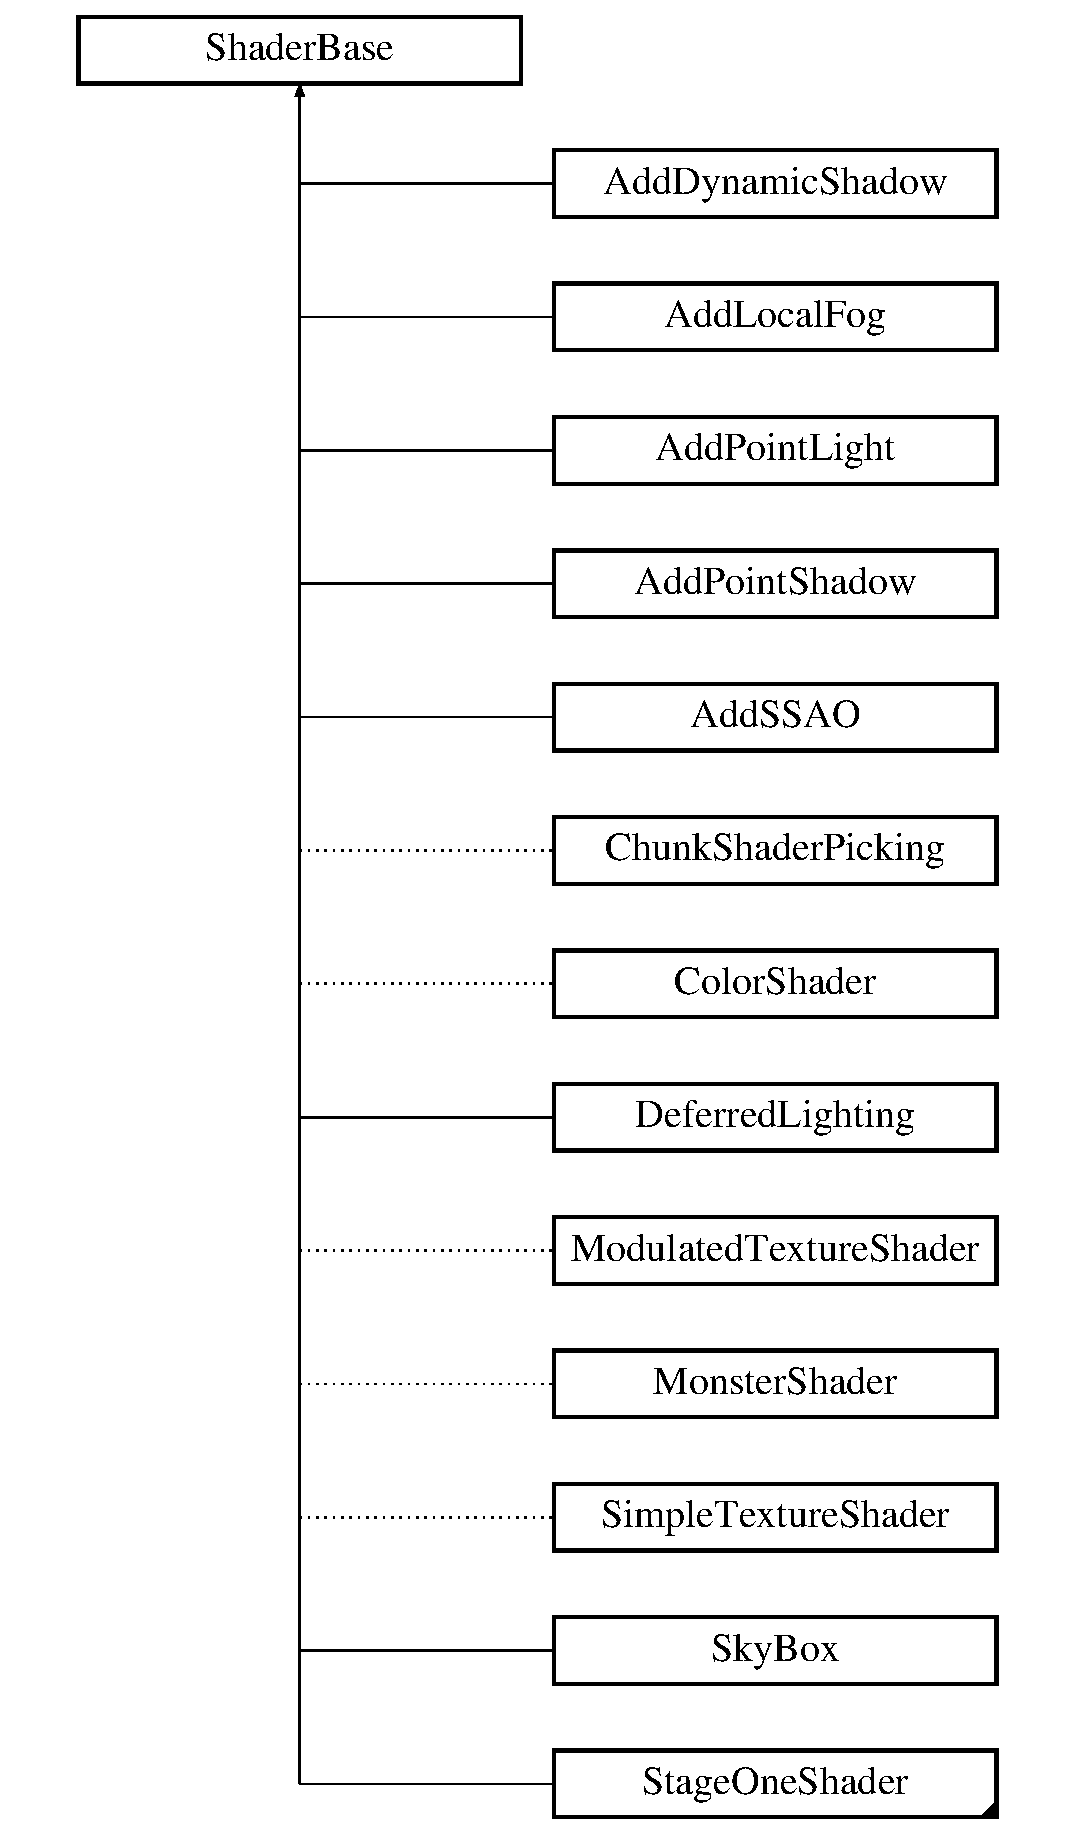
\includegraphics[height=12.000000cm]{classShaderBase}
\end{center}
\end{figure}
\subsection*{\-Public \-Member \-Functions}
\begin{DoxyCompactItemize}
\item 
\hypertarget{classShaderBase_a9dd2a538a1760b1b8744e2e0a8075d27}{void {\bfseries \-Init} (const char $\ast$debug, int vertex\-Shader\-Lines, const char $\ast$$\ast$vertex\-Shader\-Source, int fragment\-Shader\-Lines, const char $\ast$$\ast$fragment\-Shader\-Source)}\label{classShaderBase_a9dd2a538a1760b1b8744e2e0a8075d27}

\item 
\hypertarget{classShaderBase_a12ba43f4f4228bb1b759f53f9e0d9e38}{void {\bfseries \-Initglsw} (const char $\ast$debug, int vertex\-Shader\-Lines, const char $\ast$$\ast$vertex\-Shader\-Source, int fragment\-Shader\-Lines, const char $\ast$$\ast$fragment\-Shader\-Source)}\label{classShaderBase_a12ba43f4f4228bb1b759f53f9e0d9e38}

\end{DoxyCompactItemize}
\subsection*{\-Protected \-Member \-Functions}
\begin{DoxyCompactItemize}
\item 
\hypertarget{classShaderBase_a43c4aeb651eaa7d12ffa45c65cb86cc5}{\-G\-Luint {\bfseries \-Program} (void) const }\label{classShaderBase_a43c4aeb651eaa7d12ffa45c65cb86cc5}

\item 
\hypertarget{classShaderBase_abd2bd3d01dce1e25aa10d1f62216ee57}{virtual void {\bfseries \-Get\-Locations} (void)=0}\label{classShaderBase_abd2bd3d01dce1e25aa10d1f62216ee57}

\item 
\hypertarget{classShaderBase_aba35258b10e57c65fb07e3b134f1977e}{virtual void {\bfseries \-Pre\-Link\-Callback} (\-G\-Luint prg)}\label{classShaderBase_aba35258b10e57c65fb07e3b134f1977e}

\item 
\hypertarget{classShaderBase_a09935c4d278aaacbf0a0300e15ee8901}{\-G\-Lint {\bfseries \-Get\-Uniform\-Location} (const char $\ast$) const }\label{classShaderBase_a09935c4d278aaacbf0a0300e15ee8901}

\item 
\hypertarget{classShaderBase_a23ff68011100d7ccbf7beba7c898eed0}{\-G\-Lint {\bfseries \-Get\-Attrib\-Location} (const char $\ast$) const }\label{classShaderBase_a23ff68011100d7ccbf7beba7c898eed0}

\item 
\hypertarget{classShaderBase_a380d68d5caddef1507c81ea9ef83e173}{\-G\-Luint {\bfseries \-Get\-Uniform\-Block\-Index} (const char $\ast$) const }\label{classShaderBase_a380d68d5caddef1507c81ea9ef83e173}

\end{DoxyCompactItemize}


\subsection{\-Detailed \-Description}
\-Matrices used \-Some general info about how matrices are used in \-Ephenation. \-The most important transformation matrices\-: 

o \-Umodel\-Matrix o g\-View\-Matrix(in the shader\-: mat U\-B\-O\-View\-Matrix) o g\-Projection\-Matrix(in the shader\-: mat4 U\-B\-O\-Projection\-Matrix)

\-In \-Ephenation, the \-Model and \-View matrices are maintained separately as opposed to say the general convention of concatenated \-Model\-View matrix typically used in \-Open\-G\-L.

1) \-Umodel\-Matrix\-: \-The model matrix, used for the model transformations, i.\-e. from the model space of the individual \-Game elements like sky, player, etc. to the world space.

2) \-U\-B\-O\-View\-Matrix\-:\-The \-View matrix, used to transform from the world space to the camera(or eye) space. \-In this space, the camera(or eye) is at the origin, facing negative \-Z.

3) \-U\-B\-O\-Projection\-Matrix\-: \-The projection matrix.

\begin{DoxyRefDesc}{\-Todo}
\item[\hyperlink{todo__todo000001}{\-Todo}]use link, link from main page? \end{DoxyRefDesc}


\-This is an abstract shader class. \-Inherit it to create new shader programs. 

\-The documentation for this class was generated from the following files\-:\begin{DoxyCompactItemize}
\item 
shaders/shader.\-h\item 
shaders/shader.\-cpp\end{DoxyCompactItemize}

\hypertarget{classShadowMapShader}{\section{\-Shadow\-Map\-Shader \-Class \-Reference}
\label{classShadowMapShader}\index{\-Shadow\-Map\-Shader@{\-Shadow\-Map\-Shader}}
}
\-Inheritance diagram for \-Shadow\-Map\-Shader\-:\begin{figure}[H]
\begin{center}
\leavevmode
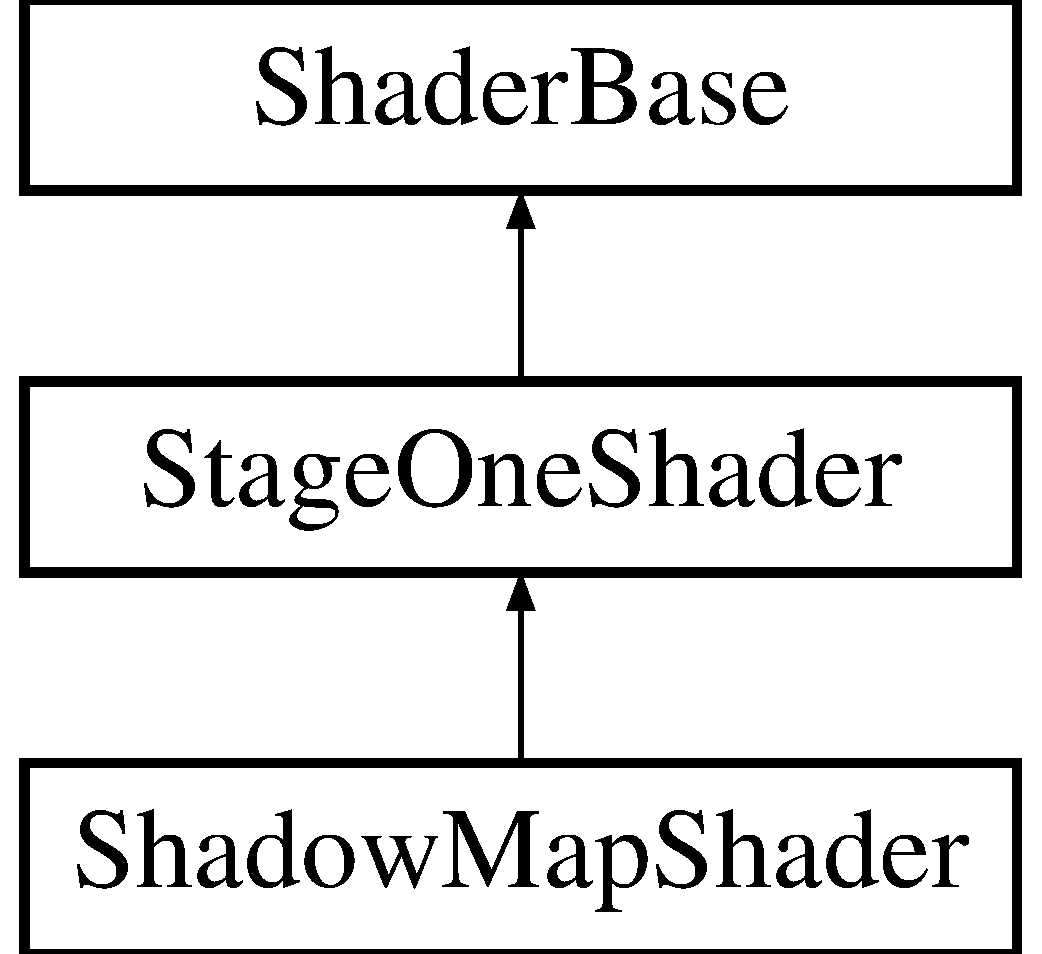
\includegraphics[height=3.000000cm]{classShadowMapShader}
\end{center}
\end{figure}
\subsection*{\-Public \-Member \-Functions}
\begin{DoxyCompactItemize}
\item 
\hypertarget{classShadowMapShader_a62b0337ad224285324617e419eb671dc}{void {\bfseries \-Model} (const glm\-::mat4 \&)}\label{classShadowMapShader_a62b0337ad224285324617e419eb671dc}

\item 
\hypertarget{classShadowMapShader_a885d50b5689ed609a8b67cbc7e78b595}{void {\bfseries \-Projection\-View} (const glm\-::mat4 \&)}\label{classShadowMapShader_a885d50b5689ed609a8b67cbc7e78b595}

\item 
\hypertarget{classShadowMapShader_a6bec41d5a6905c9c31fb276beb7ab448}{virtual void {\bfseries \-Texture\-Offset\-Multi} (float offs\-X, float offs\-Y, float mult)}\label{classShadowMapShader_a6bec41d5a6905c9c31fb276beb7ab448}

\end{DoxyCompactItemize}
\subsection*{\-Static \-Public \-Member \-Functions}
\begin{DoxyCompactItemize}
\item 
\hypertarget{classShadowMapShader_a3d11aef31beba66abbe2fc94749c9758}{static std\-::unique\-\_\-ptr\*
$<$ \hyperlink{classShadowMapShader}{\-Shadow\-Map\-Shader} $>$ {\bfseries \-Make} (void)}\label{classShadowMapShader_a3d11aef31beba66abbe2fc94749c9758}

\end{DoxyCompactItemize}
\subsection*{\-Protected \-Member \-Functions}
\begin{DoxyCompactItemize}
\item 
\hypertarget{classShadowMapShader_a17cf9dadcb7fdf7d06eb25cf1234adee}{virtual void {\bfseries \-Pre\-Link\-Callback} (\-G\-Luint prg)}\label{classShadowMapShader_a17cf9dadcb7fdf7d06eb25cf1234adee}

\end{DoxyCompactItemize}


\-The documentation for this class was generated from the following files\-:\begin{DoxyCompactItemize}
\item 
shaders/shadowmapshader.\-h\item 
shaders/shadowmapshader.\-cpp\end{DoxyCompactItemize}

\hypertarget{classShadowRender}{\section{\-Shadow\-Render \-Class \-Reference}
\label{classShadowRender}\index{\-Shadow\-Render@{\-Shadow\-Render}}
}
\subsection*{\-Public \-Member \-Functions}
\begin{DoxyCompactItemize}
\item 
\hypertarget{classShadowRender_ad1a1341925ec8819980f5c1553f380be}{{\bfseries \-Shadow\-Render} (int width, int height)}\label{classShadowRender_ad1a1341925ec8819980f5c1553f380be}

\item 
\hypertarget{classShadowRender_a52e948acef634915df96cb489f69bc1c}{void {\bfseries \-Init} ()}\label{classShadowRender_a52e948acef634915df96cb489f69bc1c}

\item 
\hypertarget{classShadowRender_aed016f7894f22533f04f52cbf33447e0}{void {\bfseries \-Render} (int width, int height, const \hyperlink{classAnimationModels}{\-Animation\-Models} $\ast$animation\-Models)}\label{classShadowRender_aed016f7894f22533f04f52cbf33447e0}

\item 
\hypertarget{classShadowRender_a3b4d1f1c5604badf5b2aaa4449451896}{void {\bfseries \-Bind\-Texture} (void) const }\label{classShadowRender_a3b4d1f1c5604badf5b2aaa4449451896}

\item 
\hypertarget{classShadowRender_a7251c69265a5a890e4237c54d9a661c3}{const glm\-::mat4 \& {\bfseries \-Get\-Pro\-View\-Matrix} (void) const }\label{classShadowRender_a7251c69265a5a890e4237c54d9a661c3}

\end{DoxyCompactItemize}


\-The documentation for this class was generated from the following files\-:\begin{DoxyCompactItemize}
\item 
shadowrender.\-h\item 
shadowrender.\-cpp\end{DoxyCompactItemize}

\hypertarget{classShadows}{\section{\-Shadows \-Class \-Reference}
\label{classShadows}\index{\-Shadows@{\-Shadows}}
}
\subsection*{\-Public \-Member \-Functions}
\begin{DoxyCompactItemize}
\item 
\hypertarget{classShadows_ab23c4ce71f75da12fcbede661e58e5b1}{void {\bfseries \-Clear} (void)}\label{classShadows_ab23c4ce71f75da12fcbede661e58e5b1}

\item 
\hypertarget{classShadows_a4eae23034eb1131810890ec8b764ea66}{void {\bfseries \-Add} (float x, float y, float z, float radius, float limit=1.\-0)}\label{classShadows_a4eae23034eb1131810890ec8b764ea66}

\item 
\hypertarget{classShadows_aff6237dabe954f9985b7b7a246e53c70}{int {\bfseries \-Get\-Count} (void) const }\label{classShadows_aff6237dabe954f9985b7b7a246e53c70}

\item 
\hypertarget{classShadows_aba6e89e2dde67a6b27f727c83846537a}{glm\-::vec4 $\ast$ {\bfseries \-Get\-List} (void)}\label{classShadows_aba6e89e2dde67a6b27f727c83846537a}

\end{DoxyCompactItemize}


\-The documentation for this class was generated from the following files\-:\begin{DoxyCompactItemize}
\item 
render.\-h\item 
render.\-cpp\end{DoxyCompactItemize}

\hypertarget{classSimpleTextureShader}{\section{\-Simple\-Texture\-Shader \-Class \-Reference}
\label{classSimpleTextureShader}\index{\-Simple\-Texture\-Shader@{\-Simple\-Texture\-Shader}}
}
\-Inheritance diagram for \-Simple\-Texture\-Shader\-:\begin{figure}[H]
\begin{center}
\leavevmode
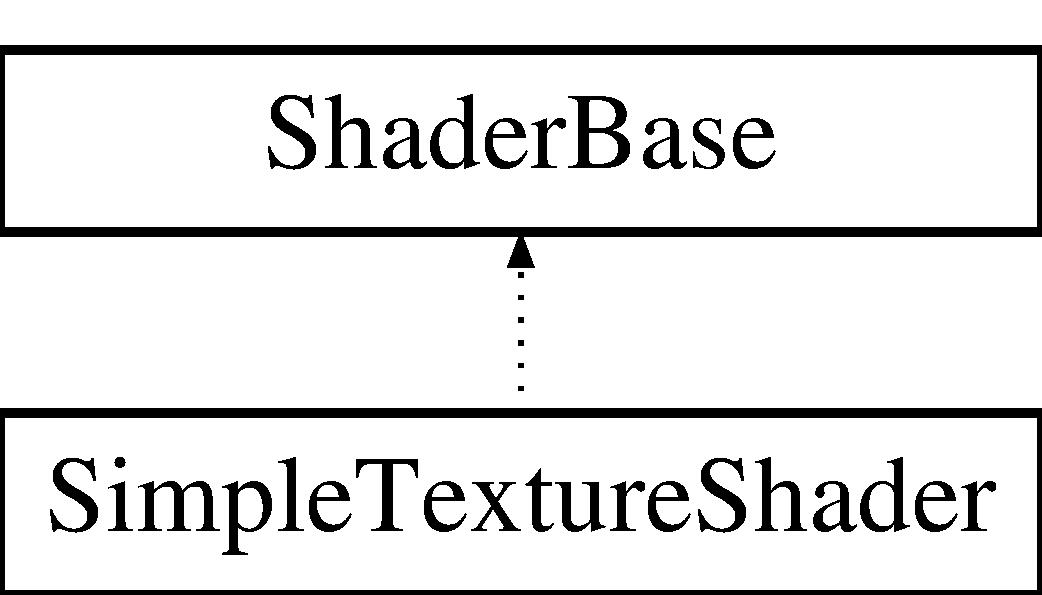
\includegraphics[height=2.000000cm]{classSimpleTextureShader}
\end{center}
\end{figure}
\subsection*{\-Public \-Member \-Functions}
\begin{DoxyCompactItemize}
\item 
\hypertarget{classSimpleTextureShader_ab1337699a07b0d95800759fa41b3dfc8}{void {\bfseries \-Enable\-Program} (void)}\label{classSimpleTextureShader_ab1337699a07b0d95800759fa41b3dfc8}

\item 
\hypertarget{classSimpleTextureShader_ac9d95b1a26fd58fea2ec8d2c4d4667e8}{void {\bfseries \-Disable\-Program} (void)}\label{classSimpleTextureShader_ac9d95b1a26fd58fea2ec8d2c4d4667e8}

\item 
\hypertarget{classSimpleTextureShader_a7af7836bf457cbe958921b5de9661393}{void {\bfseries \-Model\-View} (const glm\-::mat4 \&)}\label{classSimpleTextureShader_a7af7836bf457cbe958921b5de9661393}

\item 
\hypertarget{classSimpleTextureShader_a71c5348917015943eb937dab9e75f2bc}{void {\bfseries \-Projection} (const glm\-::mat4 \&)}\label{classSimpleTextureShader_a71c5348917015943eb937dab9e75f2bc}

\item 
\hypertarget{classSimpleTextureShader_a748c23e2920a3aabf5abaa9cf93c8629}{void {\bfseries \-Force\-Transparent} (float alpha)}\label{classSimpleTextureShader_a748c23e2920a3aabf5abaa9cf93c8629}

\item 
\hypertarget{classSimpleTextureShader_a907cc0a6b3aac300471f731df1025625}{void {\bfseries \-Texture\-Offset\-Multi} (float offs\-X, float offs\-Y, float mult)}\label{classSimpleTextureShader_a907cc0a6b3aac300471f731df1025625}

\item 
\hypertarget{classSimpleTextureShader_a76e795f797d5f866fea98d5e086fd9cf}{void {\bfseries \-Vertex\-Attrib\-Pointer} (\-G\-Lenum type, \-G\-Lint size, \-G\-Lsizei stride, const \-G\-Lvoid $\ast$pointer)}\label{classSimpleTextureShader_a76e795f797d5f866fea98d5e086fd9cf}

\item 
\hypertarget{classSimpleTextureShader_a805595227822d5e9ae6467a0de626676}{void {\bfseries \-Texture\-Attrib\-Pointer} (\-G\-Lenum type, \-G\-Lsizei stride, const \-G\-Lvoid $\ast$pointer)}\label{classSimpleTextureShader_a805595227822d5e9ae6467a0de626676}

\item 
\hypertarget{classSimpleTextureShader_ac2167e75a43cd85f3dc89a8fbcfccd09}{void {\bfseries \-Enable\-Vertex\-Attrib\-Array} (void)}\label{classSimpleTextureShader_ac2167e75a43cd85f3dc89a8fbcfccd09}

\item 
\hypertarget{classSimpleTextureShader_a360a4935810670114fab3916c7af42ae}{void {\bfseries \-Set\-Color\-Offset} (const glm\-::vec3 \&)}\label{classSimpleTextureShader_a360a4935810670114fab3916c7af42ae}

\end{DoxyCompactItemize}
\subsection*{\-Static \-Public \-Member \-Functions}
\begin{DoxyCompactItemize}
\item 
\hypertarget{classSimpleTextureShader_a84653790e0c6103c90a05094810e8fb4}{static \hyperlink{classSimpleTextureShader}{\-Simple\-Texture\-Shader} $\ast$ {\bfseries \-Make} (void)}\label{classSimpleTextureShader_a84653790e0c6103c90a05094810e8fb4}

\end{DoxyCompactItemize}


\-The documentation for this class was generated from the following files\-:\begin{DoxyCompactItemize}
\item 
shaders/\-Simple\-Texture\-Shader.\-h\item 
shaders/\-Simple\-Texture\-Shader.\-cpp\end{DoxyCompactItemize}

\hypertarget{classSkyBox}{\section{\-Sky\-Box \-Class \-Reference}
\label{classSkyBox}\index{\-Sky\-Box@{\-Sky\-Box}}
}


\-Implementation of the \-Skybox used in \-Ephenation.  




{\ttfamily \#include $<$skybox.\-h$>$}

\-Inheritance diagram for \-Sky\-Box\-:\begin{figure}[H]
\begin{center}
\leavevmode
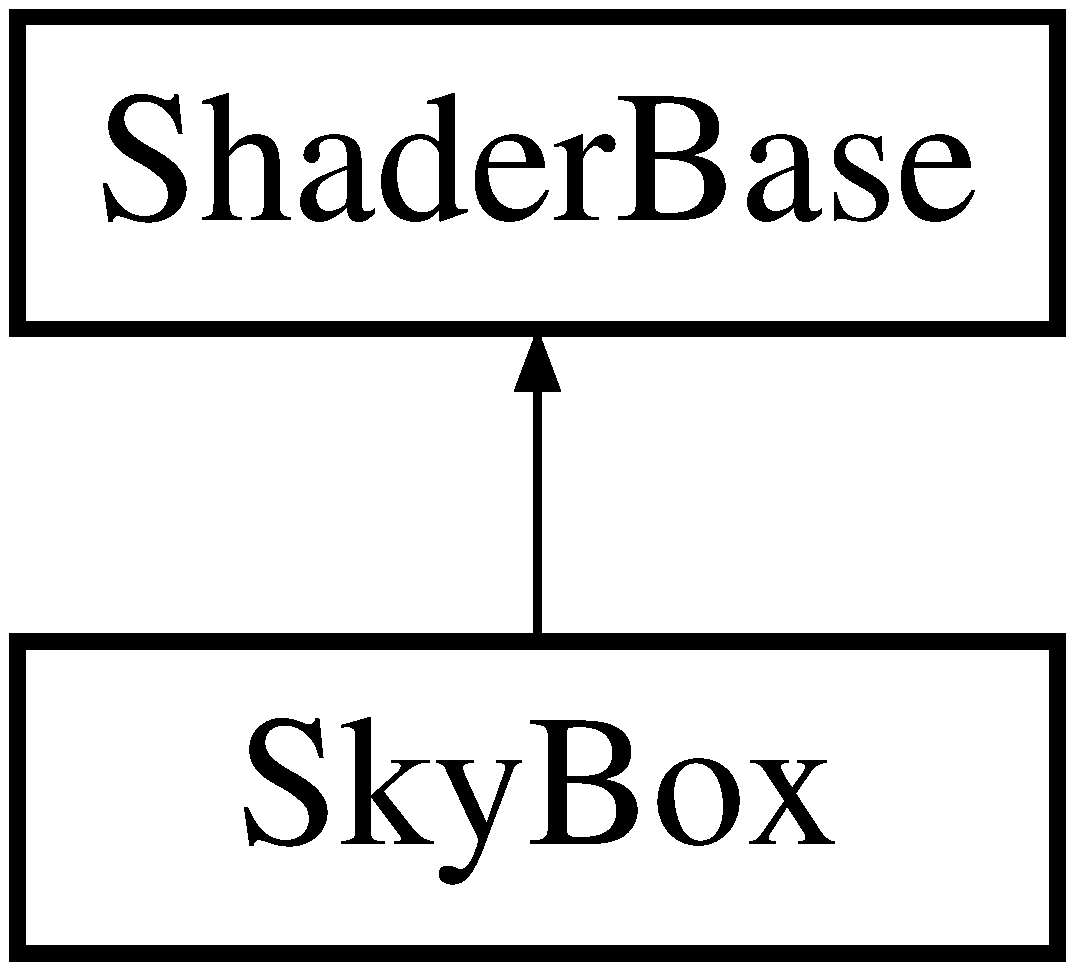
\includegraphics[height=2.000000cm]{classSkyBox}
\end{center}
\end{figure}
\subsection*{\-Public \-Member \-Functions}
\begin{DoxyCompactItemize}
\item 
\hypertarget{classSkyBox_a250406233a0f644319952fa693bd5b80}{void \hyperlink{classSkyBox_a250406233a0f644319952fa693bd5b80}{\-Init} ()}\label{classSkyBox_a250406233a0f644319952fa693bd5b80}

\begin{DoxyCompactList}\small\item\em \-Initialisation for \-Skybox shaders. \end{DoxyCompactList}\item 
void \hyperlink{classSkyBox_ab9db46f2e34683cae517ba97a44aee9e}{\-Draw} ()
\begin{DoxyCompactList}\small\item\em \-This is the \-Draw method for the \-Skybox. \end{DoxyCompactList}\end{DoxyCompactItemize}


\subsection{\-Detailed \-Description}
\-Implementation of the \-Skybox used in \-Ephenation. 

\-Vertex \-Shader\-: \-This vertex shader will only draw two triangles, limited to the part of the screen that can be affected.\-The vertex input is 0,0 in one corner and 1,1 in the other. \-Draw the quad at z -\/1, with x and y going from -\/1 to 1(and then transformed with the model matrix).

\char`\"{}pos\char`\"{} is the eye space coordinate of the vertices. \char`\"{}position\char`\"{} is the eye space value, multiplied by a large number. \-Done so that a large value is stored in the \-G-\/\-Buffer. \begin{DoxyRefDesc}{\-Todo}
\item[\hyperlink{todo__todo000004}{\-Todo}]\-: explain above better.\end{DoxyRefDesc}


\-Fragment \-Shader\-: \-Output to the \-G-\/\-Buffer 

\subsection{\-Member \-Function \-Documentation}
\hypertarget{classSkyBox_ab9db46f2e34683cae517ba97a44aee9e}{\index{\-Sky\-Box@{\-Sky\-Box}!\-Draw@{\-Draw}}
\index{\-Draw@{\-Draw}!SkyBox@{\-Sky\-Box}}
\subsubsection[{\-Draw}]{\setlength{\rightskip}{0pt plus 5cm}void {\bf \-Sky\-Box\-::\-Draw} (
\begin{DoxyParamCaption}
\item[{void}]{}
\end{DoxyParamCaption}
)}}\label{classSkyBox_ab9db46f2e34683cae517ba97a44aee9e}


\-This is the \-Draw method for the \-Skybox. 

\-The skybox is created using 4 quads, each going from -\/1.\-0 to 1.\-0. \-The quads are rotated and a box is formed. \-The model transformations(the four rotations) are done on the \-C\-P\-U as shown below. \-The view transform is then applied within the shader.

\begin{DoxyRefDesc}{\-Todo}
\item[\hyperlink{todo__todo000003}{\-Todo}]\-Move the model transforms to shader? \end{DoxyRefDesc}


\-The documentation for this class was generated from the following files\-:\begin{DoxyCompactItemize}
\item 
shaders/skybox.\-h\item 
shaders/\hyperlink{skybox_8cpp}{skybox.\-cpp}\end{DoxyCompactItemize}

\hypertarget{classSoundControl}{\section{\-Sound\-Control \-Class \-Reference}
\label{classSoundControl}\index{\-Sound\-Control@{\-Sound\-Control}}
}
\subsection*{\-Classes}
\begin{DoxyCompactItemize}
\item 
struct {\bfseries \-Music\-List}
\item 
struct {\bfseries \-Sound\-Buffer}
\item 
struct {\bfseries \-Sound\-Creature}
\item 
struct {\bfseries \-Sound\-Environment}
\item 
struct \hyperlink{structSoundControl_1_1TrigSoundItem}{\-Trig\-Sound\-Item}
\end{DoxyCompactItemize}
\subsection*{\-Public \-Types}
\begin{DoxyCompactItemize}
\item 
enum \{ \*
{\bfseries \-S\-None} =  0, 
{\bfseries \-S\-Terminate} =  1$<$$<$0, 
{\bfseries \-S\-T\-S\-Exec} =  1$<$$<$1, 
{\bfseries \-S\-Growl} =  1$<$$<$2, 
\*
{\bfseries \-S\-Player\-Hits} =  1$<$$<$3, 
{\bfseries \-S\-Monster\-Hits} =  1$<$$<$4, 
{\bfseries \-S\-Healing\-Self} =  1$<$$<$5, 
{\bfseries \-S\-Player\-Jump} =  1$<$$<$6, 
\*
{\bfseries \-S\-Player\-Land} =  1$<$$<$7, 
{\bfseries \-S\-Level\-Up} =  1$<$$<$8, 
{\bfseries \-S\-Interface\-Ping} =  1$<$$<$9, 
{\bfseries \-S\-Build\-Block} =  1$<$$<$10, 
\*
{\bfseries \-S\-Remove\-Block} =  1$<$$<$11, 
{\bfseries \-S\-Drop\-Potion} =  1$<$$<$12, 
{\bfseries \-S\-Drop\-Weapon} =  1$<$$<$13, 
{\bfseries \-S\-Drop\-Armor} =  1$<$$<$14, 
\*
{\bfseries \-S\-Drop\-Scroll} =  1$<$$<$15
 \}
\item 
enum {\bfseries \-Sound\-Fx\-Status} \{ \*
{\bfseries \-S\-Player\-Running}, 
{\bfseries \-S\-Player\-Walking}, 
{\bfseries \-S\-Player\-Feet\-In\-Water}, 
{\bfseries \-S\-Player\-Swimming}, 
\*
{\bfseries \-S\-Player\-In\-Air}, 
{\bfseries \-S\-Environment\-Echo}, 
{\bfseries \-S\-Environment\-Under\-Water}
 \}
\item 
enum {\bfseries \-Music\-Mode} \{ \*
{\bfseries \-S\-Music\-Mode\-None}, 
{\bfseries \-S\-Music\-Mode\-Silence}, 
{\bfseries \-S\-Music\-Mode\-Tourist}, 
{\bfseries \-S\-Music\-Mode\-Combat}, 
\*
{\bfseries \-S\-Music\-Mode\-Menu}, 
{\bfseries \-S\-Num\-Music\-Modes}
 \}
\item 
enum {\bfseries \-Sound\-Object} \{ \*
{\bfseries \-S\-No\-Creature}, 
{\bfseries \-S\-To\-Be\-Removed}, 
{\bfseries \-S\-Other\-Player}, 
{\bfseries \-S\-Monster}, 
\*
{\bfseries \-S\-Teleport}
 \}
\item 
\hypertarget{classSoundControl_af69a989ea5ea79299d9f05cf5ca53fe9}{typedef unsigned long {\bfseries \-Sound}}\label{classSoundControl_af69a989ea5ea79299d9f05cf5ca53fe9}

\item 
\hypertarget{classSoundControl_a12ae80d6698edc774909032635995884}{typedef int {\bfseries \-Sound\-Control\-Object}}\label{classSoundControl_a12ae80d6698edc774909032635995884}

\end{DoxyCompactItemize}
\subsection*{\-Public \-Member \-Functions}
\begin{DoxyCompactItemize}
\item 
\hypertarget{classSoundControl_ae1a682985df01f0168d0caa2b3720ad1}{void {\bfseries \-Init} (void)}\label{classSoundControl_ae1a682985df01f0168d0caa2b3720ad1}

\item 
\hypertarget{classSoundControl_adca6d26b1b2ab21c6e32bd4fdeeadc19}{void {\bfseries \-Request\-Sound} (\-Sound, bool force=false)}\label{classSoundControl_adca6d26b1b2ab21c6e32bd4fdeeadc19}

\item 
\hypertarget{classSoundControl_a985abbcd6b9da230de73ebef2246b9cc}{void {\bfseries \-Request\-Trig\-Sound} (const char $\ast$)}\label{classSoundControl_a985abbcd6b9da230de73ebef2246b9cc}

\item 
\hypertarget{classSoundControl_abf99429f897755f6ce4e9e11fb99a0a1}{void {\bfseries \-Set\-Sound\-Fx\-Status} (\-Sound\-Fx\-Status, bool)}\label{classSoundControl_abf99429f897755f6ce4e9e11fb99a0a1}

\item 
\hypertarget{classSoundControl_a87de9f20ec5cf1610884d11426bf74b1}{void {\bfseries \-Set\-Creature\-Sound} (\-Sound\-Object creature\-Type, unsigned long id, float dx, float dy, float dz, bool dead, float size)}\label{classSoundControl_a87de9f20ec5cf1610884d11426bf74b1}

\item 
\hypertarget{classSoundControl_ad497e8f68a196b808bacb8f10b500c80}{void {\bfseries \-Set\-Environment\-Sound} (\-Sound\-Object sound\-Type, unsigned long id, float dx, float dy, float dz)}\label{classSoundControl_ad497e8f68a196b808bacb8f10b500c80}

\item 
\hypertarget{classSoundControl_a7c8e1e1194ba512938b61b349051c4ea}{void {\bfseries \-Remove\-Environment\-Sound} (\-Sound\-Object, unsigned long)}\label{classSoundControl_a7c8e1e1194ba512938b61b349051c4ea}

\item 
\hypertarget{classSoundControl_a96cbb50216b7e97eafac670d4077652f}{void {\bfseries \-Remove\-Creature\-Sound} (\-Sound\-Object, unsigned long)}\label{classSoundControl_a96cbb50216b7e97eafac670d4077652f}

\item 
\hypertarget{classSoundControl_ae6ee9c713ab7dd729cfd6dff33ac044f}{void {\bfseries \-Request\-Music\-Mode} (\-Music\-Mode)}\label{classSoundControl_ae6ee9c713ab7dd729cfd6dff33ac044f}

\item 
\hypertarget{classSoundControl_ae964016f7953bd952e25fc1ab8263dfc}{void {\bfseries \-Switch\-Music\-Status} (void)}\label{classSoundControl_ae964016f7953bd952e25fc1ab8263dfc}

\end{DoxyCompactItemize}
\subsection*{\-Public \-Attributes}
\begin{DoxyCompactItemize}
\item 
\hypertarget{classSoundControl_ac30f11cd91fc72225d1d7912e566e81e}{unsigned int {\bfseries f\-Num\-Trig\-Sounds}}\label{classSoundControl_ac30f11cd91fc72225d1d7912e566e81e}

\end{DoxyCompactItemize}
\subsection*{\-Static \-Public \-Attributes}
\begin{DoxyCompactItemize}
\item 
\hypertarget{classSoundControl_aca5aba7cd50812e21ad562f5b9069339}{static \hyperlink{structSoundControl_1_1TrigSoundItem}{\-Trig\-Sound\-Item} {\bfseries f\-Trig\-Sound\-List} \mbox{[}$\,$\mbox{]}}\label{classSoundControl_aca5aba7cd50812e21ad562f5b9069339}

\end{DoxyCompactItemize}


\-The documentation for this class was generated from the following files\-:\begin{DoxyCompactItemize}
\item 
\-Sound\-Control.\-h\item 
\-Sound\-Control.\-cpp\end{DoxyCompactItemize}

\hypertarget{structChunkObject_1_1SpecialObject}{\section{\-Chunk\-Object\-:\-:\-Special\-Object \-Struct \-Reference}
\label{structChunkObject_1_1SpecialObject}\index{\-Chunk\-Object\-::\-Special\-Object@{\-Chunk\-Object\-::\-Special\-Object}}
}
\subsection*{\-Public \-Attributes}
\begin{DoxyCompactItemize}
\item 
\hypertarget{structChunkObject_1_1SpecialObject_ab89a110276d7ea1c697b27152fad3d66}{float {\bfseries ambient}}\label{structChunkObject_1_1SpecialObject_ab89a110276d7ea1c697b27152fad3d66}

\item 
\hypertarget{structChunkObject_1_1SpecialObject_aff5a1595ecf4a483d3e669a26dee4ee5}{unsigned char {\bfseries x}}\label{structChunkObject_1_1SpecialObject_aff5a1595ecf4a483d3e669a26dee4ee5}

\item 
\hypertarget{structChunkObject_1_1SpecialObject_a9290909aa98cd97a05ea5731d9d0a63c}{unsigned char {\bfseries y}}\label{structChunkObject_1_1SpecialObject_a9290909aa98cd97a05ea5731d9d0a63c}

\item 
\hypertarget{structChunkObject_1_1SpecialObject_a19f5885824f14b3df3bbc52dd22e8e86}{unsigned char {\bfseries z}}\label{structChunkObject_1_1SpecialObject_a19f5885824f14b3df3bbc52dd22e8e86}

\item 
\hypertarget{structChunkObject_1_1SpecialObject_ac897609005420295f9fa312dcb6f89b2}{unsigned char {\bfseries type}}\label{structChunkObject_1_1SpecialObject_ac897609005420295f9fa312dcb6f89b2}

\end{DoxyCompactItemize}


\-The documentation for this struct was generated from the following file\-:\begin{DoxyCompactItemize}
\item 
\-Chunk\-Object.\-h\end{DoxyCompactItemize}

\hypertarget{classSplitter}{\section{\-Splitter \-Class \-Reference}
\label{classSplitter}\index{\-Splitter@{\-Splitter}}
}


{\ttfamily \#include $<$\-Splitter.\-h$>$}

\subsection*{\-Public \-Types}
\begin{DoxyCompactItemize}
\item 
\hypertarget{classSplitter_a24341275a00c0b617655258f5372a42c}{typedef std\-::vector\*
$<$ std\-::string $>$\-::\hyperlink{classSplitter_a24341275a00c0b617655258f5372a42c}{size\-\_\-type} \hyperlink{classSplitter_a24341275a00c0b617655258f5372a42c}{size\-\_\-type}}\label{classSplitter_a24341275a00c0b617655258f5372a42c}

\begin{DoxyCompactList}\small\item\em \-Subscript type for use with operator\mbox{[}\mbox{]}. \end{DoxyCompactList}\end{DoxyCompactItemize}
\subsection*{\-Public \-Member \-Functions}
\begin{DoxyCompactItemize}
\item 
\hyperlink{classSplitter_a41eddab681f5186c74c23c4e22666a36}{\-Splitter} (const std\-::string \&src, const std\-::string \&delim)
\item 
std\-::string \& \hyperlink{classSplitter_a2023627ffc281f4adc668251141715cc}{operator\mbox{[}$\,$\mbox{]}} (\hyperlink{classSplitter_a24341275a00c0b617655258f5372a42c}{size\-\_\-type} i)
\item 
\hyperlink{classSplitter_a24341275a00c0b617655258f5372a42c}{size\-\_\-type} \hyperlink{classSplitter_acc58917adcf1da6e6dbab05354a02276}{size} () const 
\item 
void \hyperlink{classSplitter_aadcb25576bce2a54423a17a63365848f}{reset} (const std\-::string \&src, const std\-::string \&delim)
\end{DoxyCompactItemize}


\subsection{\-Detailed \-Description}
\-Maintains a collection of substrings that are delimited by a string of one or more characters 

\subsection{\-Constructor \& \-Destructor \-Documentation}
\hypertarget{classSplitter_a41eddab681f5186c74c23c4e22666a36}{\index{\-Splitter@{\-Splitter}!\-Splitter@{\-Splitter}}
\index{\-Splitter@{\-Splitter}!Splitter@{\-Splitter}}
\subsubsection[{\-Splitter}]{\setlength{\rightskip}{0pt plus 5cm}{\bf \-Splitter\-::\-Splitter} (
\begin{DoxyParamCaption}
\item[{const std\-::string \&}]{src, }
\item[{const std\-::string \&}]{delim}
\end{DoxyParamCaption}
)\hspace{0.3cm}{\ttfamily  \mbox{[}inline\mbox{]}}}}\label{classSplitter_a41eddab681f5186c74c23c4e22666a36}
\-Create and initialize a new \hyperlink{classSplitter}{\-Splitter}


\begin{DoxyParams}[1]{\-Parameters}
\mbox{\tt in}  & {\em src} & \-The string to split \\
\hline
\mbox{\tt in}  & {\em delim} & \-The delimiter to split the string around \\
\hline
\end{DoxyParams}


\subsection{\-Member \-Function \-Documentation}
\hypertarget{classSplitter_a2023627ffc281f4adc668251141715cc}{\index{\-Splitter@{\-Splitter}!operator\mbox{[}$\,$\mbox{]}@{operator[]}}
\index{operator\mbox{[}$\,$\mbox{]}@{operator[]}!Splitter@{\-Splitter}}
\subsubsection[{operator[]}]{\setlength{\rightskip}{0pt plus 5cm}std\-::string\& \-Splitter\-::operator\mbox{[}$\,$\mbox{]} (
\begin{DoxyParamCaption}
\item[{{\bf size\-\_\-type}}]{i}
\end{DoxyParamCaption}
)\hspace{0.3cm}{\ttfamily  \mbox{[}inline\mbox{]}}}}\label{classSplitter_a2023627ffc281f4adc668251141715cc}
\-Retrieve a split token at the specified index


\begin{DoxyParams}[1]{\-Parameters}
\mbox{\tt in}  & {\em i} & \-The index to search for a token \\
\hline
\end{DoxyParams}
\begin{DoxyReturn}{\-Returns}
\-The token at the specified index 
\end{DoxyReturn}

\begin{DoxyExceptions}{\-Exceptions}
{\em std\-::out\-\_\-of\-\_\-range} & \-If the index is invalid \\
\hline
\end{DoxyExceptions}
\hypertarget{classSplitter_aadcb25576bce2a54423a17a63365848f}{\index{\-Splitter@{\-Splitter}!reset@{reset}}
\index{reset@{reset}!Splitter@{\-Splitter}}
\subsubsection[{reset}]{\setlength{\rightskip}{0pt plus 5cm}void {\bf \-Splitter\-::reset} (
\begin{DoxyParamCaption}
\item[{const std\-::string \&}]{src, }
\item[{const std\-::string \&}]{delim}
\end{DoxyParamCaption}
)\hspace{0.3cm}{\ttfamily  \mbox{[}inline\mbox{]}}}}\label{classSplitter_aadcb25576bce2a54423a17a63365848f}
\-Re-\/initialize with a new soruce and delimiter


\begin{DoxyParams}[1]{\-Parameters}
\mbox{\tt in}  & {\em src} & \-The string to split \\
\hline
\mbox{\tt in}  & {\em delim} & \-The delimiter to split the string around \\
\hline
\end{DoxyParams}
\hypertarget{classSplitter_acc58917adcf1da6e6dbab05354a02276}{\index{\-Splitter@{\-Splitter}!size@{size}}
\index{size@{size}!Splitter@{\-Splitter}}
\subsubsection[{size}]{\setlength{\rightskip}{0pt plus 5cm}{\bf size\-\_\-type} {\bf \-Splitter\-::size} (
\begin{DoxyParamCaption}
{}
\end{DoxyParamCaption}
) const\hspace{0.3cm}{\ttfamily  \mbox{[}inline\mbox{]}}}}\label{classSplitter_acc58917adcf1da6e6dbab05354a02276}
\-Retrieve the number of split tokens

\begin{DoxyReturn}{\-Returns}
\-The number of split tokesn 
\end{DoxyReturn}


\-The documentation for this class was generated from the following file\-:\begin{DoxyCompactItemize}
\item 
\-Splitter.\-h\end{DoxyCompactItemize}

\hypertarget{classStageOneShader}{\section{\-Stage\-One\-Shader \-Class \-Reference}
\label{classStageOneShader}\index{\-Stage\-One\-Shader@{\-Stage\-One\-Shader}}
}
\-Inheritance diagram for \-Stage\-One\-Shader\-:\begin{figure}[H]
\begin{center}
\leavevmode
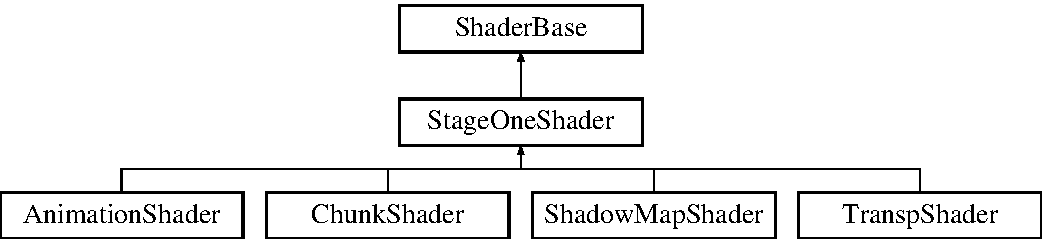
\includegraphics[height=3.000000cm]{classStageOneShader}
\end{center}
\end{figure}
\subsection*{\-Public \-Types}
\begin{DoxyCompactItemize}
\item 
enum {\bfseries \-Input\-Locations} \{ {\bfseries \-Normal}, 
{\bfseries \-Vertex}, 
{\bfseries \-Skin\-Weights}, 
{\bfseries \-Joints}
 \}
\end{DoxyCompactItemize}
\subsection*{\-Public \-Member \-Functions}
\begin{DoxyCompactItemize}
\item 
\hypertarget{classStageOneShader_ad4e7930febdc8bd6274232cca0203f12}{virtual void {\bfseries \-Model} (const glm\-::mat4 \&)=0}\label{classStageOneShader_ad4e7930febdc8bd6274232cca0203f12}

\item 
\hypertarget{classStageOneShader_a500639ba8a97e46d6b1b5f2b5815a239}{virtual void {\bfseries \-Drawing\-Water} (bool)}\label{classStageOneShader_a500639ba8a97e46d6b1b5f2b5815a239}

\item 
\hypertarget{classStageOneShader_ae53cd72ba6f7bd1db7daeec14c01ec1d}{virtual void {\bfseries \-Texture\-Offset\-Multi} (float offs\-X, float offs\-Y, float mult)}\label{classStageOneShader_ae53cd72ba6f7bd1db7daeec14c01ec1d}

\item 
\hypertarget{classStageOneShader_a3e4c603995edf86b5d4c0985bebfcb03}{virtual void {\bfseries \-Enable\-Program} (void)}\label{classStageOneShader_a3e4c603995edf86b5d4c0985bebfcb03}

\item 
\hypertarget{classStageOneShader_a722e5537b67ddb180e6e063992b78952}{void {\bfseries \-Disable\-Program} (void)}\label{classStageOneShader_a722e5537b67ddb180e6e063992b78952}

\end{DoxyCompactItemize}
\subsection*{\-Static \-Public \-Member \-Functions}
\begin{DoxyCompactItemize}
\item 
\hypertarget{classStageOneShader_ad3d7c53fc11c96c9166925e3a4fe5ba9}{static void {\bfseries \-Vertex\-Attrib\-Pointer} (int offset=0)}\label{classStageOneShader_ad3d7c53fc11c96c9166925e3a4fe5ba9}

\item 
\hypertarget{classStageOneShader_a81e968281d4547e9acb0b7e18924399d}{static void {\bfseries \-Vertex\-Attrib\-Pointer\-Skin\-Weights} (int skin\-Offset, int joint\-Offset)}\label{classStageOneShader_a81e968281d4547e9acb0b7e18924399d}

\item 
\hypertarget{classStageOneShader_a05553a57de5a17345538af0e02cf9989}{static void {\bfseries \-Enable\-Vertex\-Attrib\-Array} (bool use\-Bones=false)}\label{classStageOneShader_a05553a57de5a17345538af0e02cf9989}

\end{DoxyCompactItemize}


\-The documentation for this class was generated from the following files\-:\begin{DoxyCompactItemize}
\item 
shaders/\-Stage\-One\-Shader.\-h\item 
shaders/\-Stage\-One\-Shader.\-cpp\end{DoxyCompactItemize}

\hypertarget{structSuperChunk}{\section{\-Super\-Chunk \-Struct \-Reference}
\label{structSuperChunk}\index{\-Super\-Chunk@{\-Super\-Chunk}}
}
\subsection*{\-Classes}
\begin{DoxyCompactItemize}
\item 
struct \hyperlink{structSuperChunk_1_1chunkInfo}{chunk\-Info}
\end{DoxyCompactItemize}
\subsection*{\-Public \-Attributes}
\begin{DoxyCompactItemize}
\item 
\hypertarget{structSuperChunk_a4a559a2e7b8f19b4c284a61818736306}{unsigned int {\bfseries f\-Check\-Sum}}\label{structSuperChunk_a4a559a2e7b8f19b4c284a61818736306}

\item 
\hypertarget{structSuperChunk_a11b5ad8b0b86192cd6966f8fab0974f5}{\hyperlink{structSuperChunk_1_1chunkInfo}{chunk\-Info} {\bfseries f\-Chunk\-Info} \mbox{[}\-S\-C\-H\-\_\-\-S\-I\-Z\-E\mbox{]}\mbox{[}\-S\-C\-H\-\_\-\-S\-I\-Z\-E\mbox{]}\mbox{[}\-S\-C\-H\-\_\-\-S\-I\-Z\-E\mbox{]}}\label{structSuperChunk_a11b5ad8b0b86192cd6966f8fab0974f5}

\item 
\hypertarget{structSuperChunk_ad4ba3e96b0ec2674bcc613f309e1b4aa}{bool {\bfseries f\-Update\-Requested}}\label{structSuperChunk_ad4ba3e96b0ec2674bcc613f309e1b4aa}

\end{DoxyCompactItemize}


\-The documentation for this struct was generated from the following file\-:\begin{DoxyCompactItemize}
\item 
\-Super\-Chunk\-Manager.\-h\end{DoxyCompactItemize}

\hypertarget{classSuperChunkManager}{\section{\-Super\-Chunk\-Manager \-Class \-Reference}
\label{classSuperChunkManager}\index{\-Super\-Chunk\-Manager@{\-Super\-Chunk\-Manager}}
}
\subsection*{\-Public \-Member \-Functions}
\begin{DoxyCompactItemize}
\item 
\hypertarget{classSuperChunkManager_a63750019d96a2d6ce202e19604914a69}{bool {\bfseries \-Get\-Teleport} (unsigned char $\ast$px, unsigned char $\ast$py, unsigned char $\ast$pz, const \hyperlink{structChunkCoord}{\-Chunk\-Coord} $\ast$cc)}\label{classSuperChunkManager_a63750019d96a2d6ce202e19604914a69}

\item 
\hypertarget{classSuperChunkManager_a86babbfdea357e9e6cbdaf1028f13fa8}{void {\bfseries \-Data} (const \hyperlink{structChunkCoord}{\-Chunk\-Coord} $\ast$cc, const unsigned char $\ast$p)}\label{classSuperChunkManager_a86babbfdea357e9e6cbdaf1028f13fa8}

\end{DoxyCompactItemize}


\-The documentation for this class was generated from the following files\-:\begin{DoxyCompactItemize}
\item 
\-Super\-Chunk\-Manager.\-h\item 
\-Super\-Chunk\-Manager.\-cpp\end{DoxyCompactItemize}

\hypertarget{classstd_1_1thread}{\section{std\-:\-:thread \-Class \-Reference}
\label{classstd_1_1thread}\index{std\-::thread@{std\-::thread}}
}
\subsection*{\-Public \-Member \-Functions}
\begin{DoxyCompactItemize}
\item 
\hypertarget{classstd_1_1thread_a7a0599bdda9dfea79e48a0842626ed0d}{{\bfseries thread} (void $\ast$($\ast$func)(\hyperlink{classChunkProcess}{\-Chunk\-Process} $\ast$p), \hyperlink{classChunkProcess}{\-Chunk\-Process} $\ast$p)}\label{classstd_1_1thread_a7a0599bdda9dfea79e48a0842626ed0d}

\item 
\hypertarget{classstd_1_1thread_a8dde69771312c0d10746295bee36cf5e}{{\bfseries thread} (\hyperlink{classstd_1_1thread}{thread} \&\&other)}\label{classstd_1_1thread_a8dde69771312c0d10746295bee36cf5e}

\item 
\hypertarget{classstd_1_1thread_a3a5b3ae0b855ba2789081f2bd4871d76}{{\bfseries thread} (const \hyperlink{classstd_1_1thread}{thread} \&)}\label{classstd_1_1thread_a3a5b3ae0b855ba2789081f2bd4871d76}

\item 
\hypertarget{classstd_1_1thread_a8b81cf4d21e5f1b354c25bf7f5bfc732}{void {\bfseries join} (void)}\label{classstd_1_1thread_a8b81cf4d21e5f1b354c25bf7f5bfc732}

\item 
\hypertarget{classstd_1_1thread_a68385269c6763275611fae6959d413fc}{bool {\bfseries joinable} (void) const }\label{classstd_1_1thread_a68385269c6763275611fae6959d413fc}

\end{DoxyCompactItemize}


\-The documentation for this class was generated from the following file\-:\begin{DoxyCompactItemize}
\item 
mythread.\-h\end{DoxyCompactItemize}

\hypertarget{classTimeMeasure}{\section{\-Time\-Measure \-Class \-Reference}
\label{classTimeMeasure}\index{\-Time\-Measure@{\-Time\-Measure}}
}
\subsection*{\-Public \-Member \-Functions}
\begin{DoxyCompactItemize}
\item 
\hypertarget{classTimeMeasure_ada461c9f89dce4c52b6e30e7cf8b1750}{{\bfseries \-Time\-Measure} (const string \&title)}\label{classTimeMeasure_ada461c9f89dce4c52b6e30e7cf8b1750}

\item 
\hypertarget{classTimeMeasure_a73a09593f22bab5270cec7514a8c2771}{void {\bfseries \-Start} ()}\label{classTimeMeasure_a73a09593f22bab5270cec7514a8c2771}

\item 
\hypertarget{classTimeMeasure_a67706c32e985156d13918875cb71968d}{void {\bfseries \-Stop} (void)}\label{classTimeMeasure_a67706c32e985156d13918875cb71968d}

\end{DoxyCompactItemize}
\subsection*{\-Static \-Public \-Member \-Functions}
\begin{DoxyCompactItemize}
\item 
\hypertarget{classTimeMeasure_ab62bbe12d6a71b692560a2e076735dc6}{static void {\bfseries \-Report} (void)}\label{classTimeMeasure_ab62bbe12d6a71b692560a2e076735dc6}

\end{DoxyCompactItemize}


\-The documentation for this class was generated from the following files\-:\begin{DoxyCompactItemize}
\item 
timemeasure.\-h\item 
timemeasure.\-cpp\end{DoxyCompactItemize}

\hypertarget{classTranspShader}{\section{\-Transp\-Shader \-Class \-Reference}
\label{classTranspShader}\index{\-Transp\-Shader@{\-Transp\-Shader}}
}
\-Inheritance diagram for \-Transp\-Shader\-:\begin{figure}[H]
\begin{center}
\leavevmode
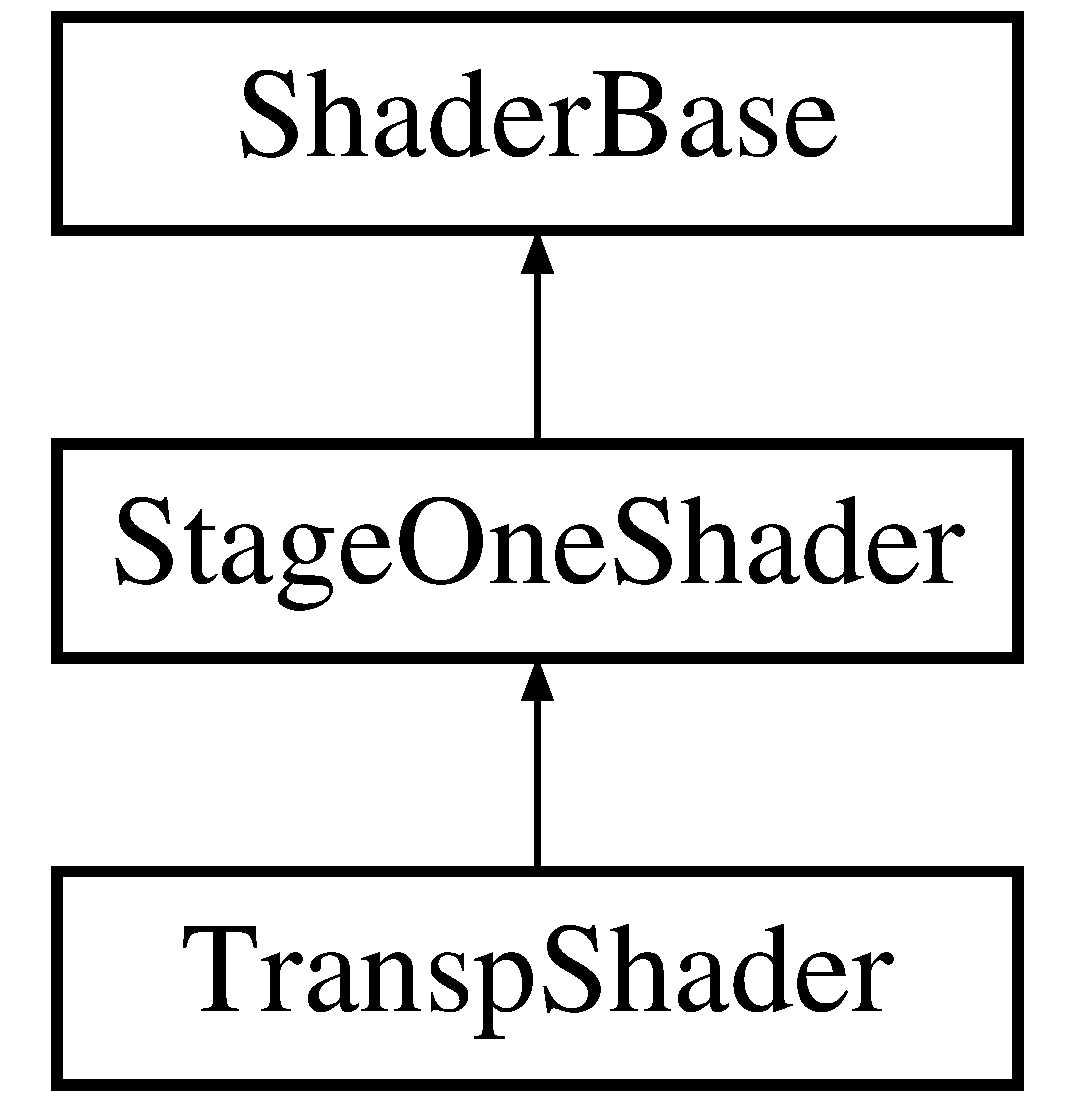
\includegraphics[height=3.000000cm]{classTranspShader}
\end{center}
\end{figure}
\subsection*{\-Public \-Member \-Functions}
\begin{DoxyCompactItemize}
\item 
\hypertarget{classTranspShader_a530c93707afcbdf03d21143020259889}{void {\bfseries \-Init} (void)}\label{classTranspShader_a530c93707afcbdf03d21143020259889}

\item 
\hypertarget{classTranspShader_aaf502a41554c7a9a6555db8fd4ae56f8}{void {\bfseries \-Model} (const glm\-::mat4 \&)}\label{classTranspShader_aaf502a41554c7a9a6555db8fd4ae56f8}

\item 
\hypertarget{classTranspShader_aaa300e0878a052d63b7c0b828cb2b6d4}{void {\bfseries \-View} (float time)}\label{classTranspShader_aaa300e0878a052d63b7c0b828cb2b6d4}

\item 
\hypertarget{classTranspShader_a59f6775b536885d5020e0b04b67aadbe}{void {\bfseries \-Projection} (float w, float h)}\label{classTranspShader_a59f6775b536885d5020e0b04b67aadbe}

\item 
\hypertarget{classTranspShader_a153486777748b97389afdabd3e575d0a}{virtual void {\bfseries \-Drawing\-Water} (bool)}\label{classTranspShader_a153486777748b97389afdabd3e575d0a}

\end{DoxyCompactItemize}
\subsection*{\-Protected \-Member \-Functions}
\begin{DoxyCompactItemize}
\item 
\hypertarget{classTranspShader_ac6532b597502b6e404c9cc5616964fd1}{virtual void {\bfseries \-Pre\-Link\-Callback} (\-G\-Luint prg)}\label{classTranspShader_ac6532b597502b6e404c9cc5616964fd1}

\end{DoxyCompactItemize}


\-The documentation for this class was generated from the following files\-:\begin{DoxyCompactItemize}
\item 
shaders/\-Transp\-Shader.\-h\item 
shaders/\-Transp\-Shader.\-cpp\end{DoxyCompactItemize}

\hypertarget{classTree}{\section{\-Tree \-Class \-Reference}
\label{classTree}\index{\-Tree@{\-Tree}}
}
\subsection*{\-Public \-Member \-Functions}
\begin{DoxyCompactItemize}
\item 
\hypertarget{classTree_ad25b4855df1c9398269ba0a3fac9dccd}{void {\bfseries \-Init} (int num\-Iter, int branching, float height)}\label{classTree_ad25b4855df1c9398269ba0a3fac9dccd}

\item 
\hypertarget{classTree_add6dbeaf337c9bf0756cc91a9887d0e0}{void {\bfseries \-Draw} (void) const }\label{classTree_add6dbeaf337c9bf0756cc91a9887d0e0}

\end{DoxyCompactItemize}
\subsection*{\-Static \-Public \-Member \-Functions}
\begin{DoxyCompactItemize}
\item 
\hypertarget{classTree_ad97df9ca684657912b5da40a0b973501}{static void {\bfseries \-Init\-Static} ()}\label{classTree_ad97df9ca684657912b5da40a0b973501}

\end{DoxyCompactItemize}
\subsection*{\-Static \-Public \-Attributes}
\begin{DoxyCompactItemize}
\item 
\hypertarget{classTree_a111d4234ca7e1ac7320e599502940eec}{static \hyperlink{classTree}{\-Tree} {\bfseries sf\-Big\-Tree}}\label{classTree_a111d4234ca7e1ac7320e599502940eec}

\item 
\hypertarget{classTree_aa643295314dc011f7890dca07a1a5888}{static \hyperlink{classTree}{\-Tree} {\bfseries sf\-Medium\-Tree}}\label{classTree_aa643295314dc011f7890dca07a1a5888}

\item 
\hypertarget{classTree_a9d8547e8c76e20fce3914529de4d42ed}{static \hyperlink{classTree}{\-Tree} {\bfseries sf\-Small\-Tree}}\label{classTree_a9d8547e8c76e20fce3914529de4d42ed}

\end{DoxyCompactItemize}


\-The documentation for this class was generated from the following files\-:\begin{DoxyCompactItemize}
\item 
shapes/\-Tree.\-h\item 
shapes/\-Tree.\-cpp\end{DoxyCompactItemize}

\hypertarget{structTriangleSurfacef}{\section{\-Triangle\-Surfacef \-Struct \-Reference}
\label{structTriangleSurfacef}\index{\-Triangle\-Surfacef@{\-Triangle\-Surfacef}}
}
\subsection*{\-Public \-Attributes}
\begin{DoxyCompactItemize}
\item 
\hypertarget{structTriangleSurfacef_af477eca15a64fa610c0704ba2cc5fa46}{\hyperlink{structVertexDataf}{\-Vertex\-Dataf} {\bfseries v} \mbox{[}3\mbox{]}}\label{structTriangleSurfacef_af477eca15a64fa610c0704ba2cc5fa46}

\end{DoxyCompactItemize}


\-The documentation for this struct was generated from the following file\-:\begin{DoxyCompactItemize}
\item 
primitives.\-h\end{DoxyCompactItemize}

\hypertarget{structSoundControl_1_1TrigSoundItem}{\section{\-Sound\-Control\-:\-:\-Trig\-Sound\-Item \-Struct \-Reference}
\label{structSoundControl_1_1TrigSoundItem}\index{\-Sound\-Control\-::\-Trig\-Sound\-Item@{\-Sound\-Control\-::\-Trig\-Sound\-Item}}
}
\subsection*{\-Public \-Attributes}
\begin{DoxyCompactItemize}
\item 
\hypertarget{structSoundControl_1_1TrigSoundItem_a92454c67dde49ccd415f37e04bdd4dfc}{char {\bfseries id} \mbox{[}5\mbox{]}}\label{structSoundControl_1_1TrigSoundItem_a92454c67dde49ccd415f37e04bdd4dfc}

\item 
\hypertarget{structSoundControl_1_1TrigSoundItem_a4519e73384fda899a43a7e0facaf9543}{const char $\ast$ {\bfseries file\-Name}}\label{structSoundControl_1_1TrigSoundItem_a4519e73384fda899a43a7e0facaf9543}

\item 
\hypertarget{structSoundControl_1_1TrigSoundItem_a19d2b8df1fc90cc00fb96f3698620299}{const char $\ast$ {\bfseries description}}\label{structSoundControl_1_1TrigSoundItem_a19d2b8df1fc90cc00fb96f3698620299}

\end{DoxyCompactItemize}


\-The documentation for this struct was generated from the following file\-:\begin{DoxyCompactItemize}
\item 
\-Sound\-Control.\-h\end{DoxyCompactItemize}

\hypertarget{classTSExec}{\section{\-T\-S\-Exec \-Class \-Reference}
\label{classTSExec}\index{\-T\-S\-Exec@{\-T\-S\-Exec}}
}
\subsection*{\-Public \-Member \-Functions}
\begin{DoxyCompactItemize}
\item 
\hypertarget{classTSExec_a30a7892f85a414658a37ca1db88eacb3}{void {\bfseries \-Init} (void)}\label{classTSExec_a30a7892f85a414658a37ca1db88eacb3}

\end{DoxyCompactItemize}
\subsection*{\-Static \-Public \-Attributes}
\begin{DoxyCompactItemize}
\item 
\hypertarget{classTSExec_a6c2bf008825ec4bfbaf3d3af07fc2c43}{static \hyperlink{classTSExec}{\-T\-S\-Exec} {\bfseries g\-T\-S\-Exec}}\label{classTSExec_a6c2bf008825ec4bfbaf3d3af07fc2c43}

\end{DoxyCompactItemize}


\-The documentation for this class was generated from the following files\-:\begin{DoxyCompactItemize}
\item 
\-T\-S\-Exec.\-h\item 
\-T\-S\-Exec.\-cpp\end{DoxyCompactItemize}

\hypertarget{classUniformBuffer}{\section{\-Uniform\-Buffer \-Class \-Reference}
\label{classUniformBuffer}\index{\-Uniform\-Buffer@{\-Uniform\-Buffer}}
}
\subsection*{\-Public \-Member \-Functions}
\begin{DoxyCompactItemize}
\item 
\hypertarget{classUniformBuffer_a8f747583602c1a409c86ad789a8b6c21}{void {\bfseries \-Init} ()}\label{classUniformBuffer_a8f747583602c1a409c86ad789a8b6c21}

\item 
\hypertarget{classUniformBuffer_a6288ae976b7d0706cbbd5b5b9c2b03f0}{void {\bfseries \-Update} (void)}\label{classUniformBuffer_a6288ae976b7d0706cbbd5b5b9c2b03f0}

\item 
\hypertarget{classUniformBuffer_a05742920d4e64793fa42d872564cdc25}{void {\bfseries \-Uniform\-Block\-Binding} (\-G\-Luint program, \-G\-Luint idx)}\label{classUniformBuffer_a05742920d4e64793fa42d872564cdc25}

\item 
\hypertarget{classUniformBuffer_a9b43415a0fea05ec45dd37c870a8f781}{void {\bfseries \-Camera} (const glm\-::vec4 \&)}\label{classUniformBuffer_a9b43415a0fea05ec45dd37c870a8f781}

\end{DoxyCompactItemize}


\-The documentation for this class was generated from the following files\-:\begin{DoxyCompactItemize}
\item 
uniformbuffer.\-h\item 
uniformbuffer.\-cpp\end{DoxyCompactItemize}

\hypertarget{classstd_1_1unique__lock}{\section{std\-:\-:unique\-\_\-lock$<$ \-T $>$ \-Class \-Template \-Reference}
\label{classstd_1_1unique__lock}\index{std\-::unique\-\_\-lock$<$ T $>$@{std\-::unique\-\_\-lock$<$ T $>$}}
}
\subsection*{\-Public \-Member \-Functions}
\begin{DoxyCompactItemize}
\item 
\hypertarget{classstd_1_1unique__lock_af49fc0cbc48df88db2a2483739c6c8f2}{{\bfseries unique\-\_\-lock} (\-T \&lock)}\label{classstd_1_1unique__lock_af49fc0cbc48df88db2a2483739c6c8f2}

\end{DoxyCompactItemize}
\subsection*{\-Public \-Attributes}
\begin{DoxyCompactItemize}
\item 
\hypertarget{classstd_1_1unique__lock_aef428f6730b325c03236079cc367a264}{\-T $\ast$ {\bfseries f\-Lock}}\label{classstd_1_1unique__lock_aef428f6730b325c03236079cc367a264}

\end{DoxyCompactItemize}
\subsubsection*{template$<$class \-T$>$ class std\-::unique\-\_\-lock$<$ T $>$}



\-The documentation for this class was generated from the following file\-:\begin{DoxyCompactItemize}
\item 
mythread.\-h\end{DoxyCompactItemize}

\hypertarget{structvertex}{\section{vertex \-Struct \-Reference}
\label{structvertex}\index{vertex@{vertex}}
}
\subsection*{\-Public \-Attributes}
\begin{DoxyCompactItemize}
\item 
\hypertarget{structvertex_a58b1910ce8ffc1cb2ee833c81b795fdf}{char {\bfseries v} \mbox{[}3\mbox{]}}\label{structvertex_a58b1910ce8ffc1cb2ee833c81b795fdf}

\item 
\hypertarget{structvertex_a05a5118bf20cb54f1b563f7f934ebc6a}{char {\bfseries t} \mbox{[}2\mbox{]}}\label{structvertex_a05a5118bf20cb54f1b563f7f934ebc6a}

\item 
\hypertarget{structvertex_ad387e5f1efc55b69b9c3380d30b1109a}{float {\bfseries v} \mbox{[}2\mbox{]}}\label{structvertex_ad387e5f1efc55b69b9c3380d30b1109a}

\item 
\hypertarget{structvertex_a808db5683e2f29c98a6456827a11e86c}{float {\bfseries t} \mbox{[}2\mbox{]}}\label{structvertex_a808db5683e2f29c98a6456827a11e86c}

\end{DoxyCompactItemize}


\-The documentation for this struct was generated from the following files\-:\begin{DoxyCompactItemize}
\item 
\-Building\-Blocks.\-cpp\item 
\-Draw\-Texture.\-cpp\item 
\-Health\-Bar.\-cpp\item 
shapes/quad.\-cpp\end{DoxyCompactItemize}

\hypertarget{structVertexDataf}{\section{\-Vertex\-Dataf \-Struct \-Reference}
\label{structVertexDataf}\index{\-Vertex\-Dataf@{\-Vertex\-Dataf}}
}
\subsection*{\-Public \-Member \-Functions}
\begin{DoxyCompactItemize}
\item 
\hypertarget{structVertexDataf_a152d55b4b719c995bda6671ba53c2507}{void {\bfseries \-Set\-Texture} (float x, float y)}\label{structVertexDataf_a152d55b4b719c995bda6671ba53c2507}

\item 
\hypertarget{structVertexDataf_a7512982046d50ccabab8436f01e959c1}{void {\bfseries \-Set\-Texture} (const glm\-::vec2 \&texture)}\label{structVertexDataf_a7512982046d50ccabab8436f01e959c1}

\item 
\hypertarget{structVertexDataf_a19fb84e7115428dff721f840532cf0f2}{glm\-::vec2 {\bfseries \-Get\-Texture} (void) const }\label{structVertexDataf_a19fb84e7115428dff721f840532cf0f2}

\item 
\hypertarget{structVertexDataf_af236fb27ae07a90ca4ab087f067d8ff4}{void {\bfseries \-Set\-Intensity} (unsigned char intensity)}\label{structVertexDataf_af236fb27ae07a90ca4ab087f067d8ff4}

\item 
\hypertarget{structVertexDataf_af09ffe52e0414d070d56198d5b7934fd}{unsigned char {\bfseries \-Get\-Intensity} (void) const }\label{structVertexDataf_af09ffe52e0414d070d56198d5b7934fd}

\item 
\hypertarget{structVertexDataf_a9ad2b6382c957ed77e7d082edcb92253}{void {\bfseries \-Set\-Ambient} (unsigned char ambient)}\label{structVertexDataf_a9ad2b6382c957ed77e7d082edcb92253}

\item 
\hypertarget{structVertexDataf_ab1743d9fec2952c29564511929dc38bf}{void {\bfseries \-Set\-Normal} (\hyperlink{unionPickingData}{\-Picking\-Data} data)}\label{structVertexDataf_ab1743d9fec2952c29564511929dc38bf}

\item 
\hypertarget{structVertexDataf_ac33bd11f533971946c18c82e5eb277fc}{void {\bfseries \-Set\-Normal} (const glm\-::vec3 \&n)}\label{structVertexDataf_ac33bd11f533971946c18c82e5eb277fc}

\item 
\hypertarget{structVertexDataf_a94b8bce2afb9f8ce5b38ed86d07abb53}{glm\-::vec3 {\bfseries \-Get\-Normal} (void) const }\label{structVertexDataf_a94b8bce2afb9f8ce5b38ed86d07abb53}

\item 
\hypertarget{structVertexDataf_a1d99ccc06ecf40ee026cbc6e98b26bc0}{void {\bfseries \-Set\-Vertex} (float x, float y, float z)}\label{structVertexDataf_a1d99ccc06ecf40ee026cbc6e98b26bc0}

\item 
\hypertarget{structVertexDataf_a3db40b1dda607d80743b25be545dfc1b}{void {\bfseries \-Set\-Vertex} (const glm\-::vec3 \&v)}\label{structVertexDataf_a3db40b1dda607d80743b25be545dfc1b}

\item 
\hypertarget{structVertexDataf_afcc60d12a1ddebd26b480b94d435961c}{glm\-::vec3 {\bfseries \-Get\-Vertex} ()}\label{structVertexDataf_afcc60d12a1ddebd26b480b94d435961c}

\item 
\hypertarget{structVertexDataf_aaa7543edaac396c7de761c711471ca53}{bool {\bfseries \-Less\-Vertex} (const \hyperlink{structVertexDataf}{\-Vertex\-Dataf} $\ast$other)}\label{structVertexDataf_aaa7543edaac396c7de761c711471ca53}

\item 
\hypertarget{structVertexDataf_ab12a4a8cf155bd05b229df8c57226670}{{\bfseries \-Vertex\-Dataf} (const glm\-::vec3 \&normal, const glm\-::vec2 \&texture, const glm\-::vec3 \hyperlink{structvertex}{vertex}, unsigned char intensity, unsigned char ambient)}\label{structVertexDataf_ab12a4a8cf155bd05b229df8c57226670}

\end{DoxyCompactItemize}
\subsection*{\-Static \-Public \-Member \-Functions}
\begin{DoxyCompactItemize}
\item 
\hypertarget{structVertexDataf_a188acd301ca1aa3564758e1f845fb078}{static void $\ast$ {\bfseries \-Get\-Texture\-Offset} (void)}\label{structVertexDataf_a188acd301ca1aa3564758e1f845fb078}

\item 
\hypertarget{structVertexDataf_a13a4f35ed3215acf6352b958ef921f08}{static void $\ast$ {\bfseries \-Get\-Intensity\-Offset} (void)}\label{structVertexDataf_a13a4f35ed3215acf6352b958ef921f08}

\item 
\hypertarget{structVertexDataf_a192cb6687897de52c321d7038ef0c8b5}{static void $\ast$ {\bfseries \-Get\-Normal\-Offset} (void)}\label{structVertexDataf_a192cb6687897de52c321d7038ef0c8b5}

\item 
\hypertarget{structVertexDataf_a37474c2b710e411be42cb6c89371e8b8}{static void $\ast$ {\bfseries \-Get\-Vertex\-Offset} (void)}\label{structVertexDataf_a37474c2b710e411be42cb6c89371e8b8}

\end{DoxyCompactItemize}


\-The documentation for this struct was generated from the following file\-:\begin{DoxyCompactItemize}
\item 
primitives.\-h\end{DoxyCompactItemize}

\hypertarget{classWorstTime}{\section{\-Worst\-Time \-Class \-Reference}
\label{classWorstTime}\index{\-Worst\-Time@{\-Worst\-Time}}
}
\subsection*{\-Public \-Member \-Functions}
\begin{DoxyCompactItemize}
\item 
\hypertarget{classWorstTime_a9b1166c0c890e668c65d186452219d45}{{\bfseries \-Worst\-Time} (const std\-::string \&title)}\label{classWorstTime_a9b1166c0c890e668c65d186452219d45}

\item 
\hypertarget{classWorstTime_a5f2c483f9a772f29bb1c57812f2fa398}{void {\bfseries \-Start} ()}\label{classWorstTime_a5f2c483f9a772f29bb1c57812f2fa398}

\item 
\hypertarget{classWorstTime_aaa5040c2cc64fe63c3ebfeb30a3ccde1}{void {\bfseries \-Stop} (void)}\label{classWorstTime_aaa5040c2cc64fe63c3ebfeb30a3ccde1}

\item 
\hypertarget{classWorstTime_ad9ae96ae08569b41ea153e330f7eb5a7}{double {\bfseries \-Get} (void) const }\label{classWorstTime_ad9ae96ae08569b41ea153e330f7eb5a7}

\end{DoxyCompactItemize}
\subsection*{\-Static \-Public \-Member \-Functions}
\begin{DoxyCompactItemize}
\item 
\hypertarget{classWorstTime_a47bf3316c1c5fe16fef899c8cfa17c64}{static void {\bfseries \-Report} (void)}\label{classWorstTime_a47bf3316c1c5fe16fef899c8cfa17c64}

\end{DoxyCompactItemize}


\-The documentation for this class was generated from the following files\-:\begin{DoxyCompactItemize}
\item 
worsttime.\-h\item 
worsttime.\-cpp\end{DoxyCompactItemize}

\chapter{\-File \-Documentation}
\hypertarget{skybox_8cpp}{\section{shaders/skybox.cpp \-File \-Reference}
\label{skybox_8cpp}\index{shaders/skybox.\-cpp@{shaders/skybox.\-cpp}}
}


vertex\-Shader\-Source is the vertex shader for the skybox  


{\ttfamily \#include $<$\-G\-L/glew.\-h$>$}\*
{\ttfamily \#include $<$stdio.\-h$>$}\*
{\ttfamily \#include $<$stdlib.\-h$>$}\*
{\ttfamily \#include $<$glm/glm.\-hpp$>$}\*
{\ttfamily \#include $<$glm/gtc/matrix\-\_\-transform.\-hpp$>$}\*
{\ttfamily \#include \char`\"{}../primitives.\-h\char`\"{}}\*
{\ttfamily \#include \char`\"{}skybox.\-h\char`\"{}}\*
{\ttfamily \#include \char`\"{}../ui/\-Error.\-h\char`\"{}}\*
{\ttfamily \#include \char`\"{}../uniformbuffer.\-h\char`\"{}}\*
{\ttfamily \#include \char`\"{}../shapes/quad.\-h\char`\"{}}\*
{\ttfamily \#include \char`\"{}../player.\-h\char`\"{}}\*
{\ttfamily \#include \char`\"{}../textures.\-h\char`\"{}}\*


\subsection{\-Detailed \-Description}
vertex\-Shader\-Source is the vertex shader for the skybox \hyperlink{}{vertex shader will only draw two triangles, limited to the part of the screen that can be affected. \-The vertex input is 0,0 in one corner and 1,1 in the other. \-Draw the quad at z -\/1, with x and y going from -\/1 to 1 (and then transformed with the model matrix).  todo 2. }
\hypertarget{simplexnoise1234_8cpp}{\section{simplexnoise1234.\-cpp \-File \-Reference}
\label{simplexnoise1234_8cpp}\index{simplexnoise1234.\-cpp@{simplexnoise1234.\-cpp}}
}


\-C implementation of \-Perlin \-Simplex \-Noise over 1,2,3, and 4 dimensions.  


{\ttfamily \#include \char`\"{}simplexnoise1234.\-h\char`\"{}}\*
\subsection*{\-Defines}
\begin{DoxyCompactItemize}
\item 
\hypertarget{simplexnoise1234_8cpp_ae426292a2a2cac396a07776ed99d6d3f}{\#define {\bfseries \-F\-A\-S\-T\-F\-L\-O\-O\-R}(x)~( ((x)$>$0) ? ((int)x) \-: (((int)x)-\/1) )}\label{simplexnoise1234_8cpp_ae426292a2a2cac396a07776ed99d6d3f}

\item 
\hypertarget{simplexnoise1234_8cpp_a5368759862ac5fb38772b91eace1205c}{\#define {\bfseries \-F2}~0.\-366025403f}\label{simplexnoise1234_8cpp_a5368759862ac5fb38772b91eace1205c}

\item 
\hypertarget{simplexnoise1234_8cpp_ae62138575e5117b9426bd8bb1830e036}{\#define {\bfseries \-G2}~0.\-211324865f}\label{simplexnoise1234_8cpp_ae62138575e5117b9426bd8bb1830e036}

\item 
\hypertarget{simplexnoise1234_8cpp_a79fc770a19406e6876ff9ffd6ce66f3d}{\#define {\bfseries \-F3}~0.\-333333333f}\label{simplexnoise1234_8cpp_a79fc770a19406e6876ff9ffd6ce66f3d}

\item 
\hypertarget{simplexnoise1234_8cpp_aa18956b1e077aaf1b24bcb4b7eb841f5}{\#define {\bfseries \-G3}~0.\-166666667f}\label{simplexnoise1234_8cpp_aa18956b1e077aaf1b24bcb4b7eb841f5}

\item 
\hypertarget{simplexnoise1234_8cpp_a7fd7918aa90b0ce1dc7ca9fe7a00e9fb}{\#define {\bfseries \-F4}~0.\-309016994f}\label{simplexnoise1234_8cpp_a7fd7918aa90b0ce1dc7ca9fe7a00e9fb}

\item 
\hypertarget{simplexnoise1234_8cpp_a6f984a8b01aafc34122cc8bc0d9d5691}{\#define {\bfseries \-G4}~0.\-138196601f}\label{simplexnoise1234_8cpp_a6f984a8b01aafc34122cc8bc0d9d5691}

\end{DoxyCompactItemize}
\subsection*{\-Functions}
\begin{DoxyCompactItemize}
\item 
\hypertarget{simplexnoise1234_8cpp_aea4b3b0e8f5296c7ad441d76a12ac998}{float {\bfseries grad1} (int hash, float x)}\label{simplexnoise1234_8cpp_aea4b3b0e8f5296c7ad441d76a12ac998}

\item 
\hypertarget{simplexnoise1234_8cpp_a637bfdf1f2ebdbb3391a5e4e5ef0fc2c}{float {\bfseries grad2} (int hash, float x, float y)}\label{simplexnoise1234_8cpp_a637bfdf1f2ebdbb3391a5e4e5ef0fc2c}

\item 
\hypertarget{simplexnoise1234_8cpp_ab17c86b1b153b31f95450884bbc636d0}{float {\bfseries grad3} (int hash, float x, float y, float z)}\label{simplexnoise1234_8cpp_ab17c86b1b153b31f95450884bbc636d0}

\item 
\hypertarget{simplexnoise1234_8cpp_ac83dd72e9b0dc41f7a885a674731a85b}{float {\bfseries grad4} (int hash, float x, float y, float z, float t)}\label{simplexnoise1234_8cpp_ac83dd72e9b0dc41f7a885a674731a85b}

\item 
float \hyperlink{simplexnoise1234_8cpp_a6f4e23028ecdc2d48e0b577645db8ee9}{snoise1} (float x)
\item 
\hypertarget{simplexnoise1234_8cpp_a537c5b1874971a64686869c81d182047}{float {\bfseries snoise2} (float x, float y)}\label{simplexnoise1234_8cpp_a537c5b1874971a64686869c81d182047}

\item 
\hypertarget{simplexnoise1234_8cpp_ab494601cb43bd5e9cb6f2f0c04c272cc}{float {\bfseries snoise3} (float x, float y, float z)}\label{simplexnoise1234_8cpp_ab494601cb43bd5e9cb6f2f0c04c272cc}

\item 
\hypertarget{simplexnoise1234_8cpp_a7961f9f2215fb6e09f40f0fc5d0e17e8}{float {\bfseries snoise4} (float x, float y, float z, float w)}\label{simplexnoise1234_8cpp_a7961f9f2215fb6e09f40f0fc5d0e17e8}

\end{DoxyCompactItemize}
\subsection*{\-Variables}
\begin{DoxyCompactItemize}
\item 
unsigned char {\bfseries perm} \mbox{[}512\mbox{]}
\end{DoxyCompactItemize}


\subsection{\-Detailed \-Description}
\-C implementation of \-Perlin \-Simplex \-Noise over 1,2,3, and 4 dimensions. \begin{DoxyAuthor}{\-Author}
\-Stefan \-Gustavson (\href{mailto:stegu@itn.liu.se}{\tt stegu@itn.\-liu.\-se}) 
\end{DoxyAuthor}


\subsection{\-Function \-Documentation}
\hypertarget{simplexnoise1234_8cpp_a6f4e23028ecdc2d48e0b577645db8ee9}{\index{simplexnoise1234.\-cpp@{simplexnoise1234.\-cpp}!snoise1@{snoise1}}
\index{snoise1@{snoise1}!simplexnoise1234.cpp@{simplexnoise1234.\-cpp}}
\subsubsection[{snoise1}]{\setlength{\rightskip}{0pt plus 5cm}float {\bf snoise1} (
\begin{DoxyParamCaption}
\item[{float}]{x}
\end{DoxyParamCaption}
)}}\label{simplexnoise1234_8cpp_a6f4e23028ecdc2d48e0b577645db8ee9}
1\-D, 2\-D, 3\-D and 4\-D float \-Perlin simplex noise 

\subsection{\-Variable \-Documentation}
\hypertarget{simplexnoise1234_8cpp_a4dd493b13a563328213f20f0d9ebb43e}{\index{simplexnoise1234.\-cpp@{simplexnoise1234.\-cpp}!perm@{perm}}
\index{perm@{perm}!simplexnoise1234.cpp@{simplexnoise1234.\-cpp}}
\subsubsection[{perm}]{\setlength{\rightskip}{0pt plus 5cm}unsigned char perm\mbox{[}512\mbox{]}}}\label{simplexnoise1234_8cpp_a4dd493b13a563328213f20f0d9ebb43e}
{\bfseries \-Initial value\-:}
\begin{DoxyCode}
 {151,160,137,91,90,15,
                           131,13,201,95,96,53,194,233,7,225,140,36,103,30,69,
      142,8,99,37,240,21,10,23,
                           190, 6,148,247,120,234,75,0,26,197,62,94,252,219,203
      ,117,35,11,32,57,177,33,
                           88,237,149,56,87,174,20,125,136,171,168, 68,175,74,
      165,71,134,139,48,27,166,
                           77,146,158,231,83,111,229,122,60,211,133,230,220,105
      ,92,41,55,46,245,40,244,
                           102,143,54, 65,25,63,161, 1,216,80,73,209,76,132,187
      ,208, 89,18,169,200,196,
                           135,130,116,188,159,86,164,100,109,198,173,186, 3,64
      ,52,217,226,250,124,123,
                           5,202,38,147,118,126,255,82,85,212,207,206,59,227,47
      ,16,58,17,182,189,28,42,
                           223,183,170,213,119,248,152, 2,44,154,163, 70,221,
      153,101,155,167, 43,172,9,
                           129,22,39,253, 19,98,108,110,79,113,224,232,178,185,
       112,104,218,246,97,228,
                           251,34,242,193,238,210,144,12,191,179,162,241, 81,51
      ,145,235,249,14,239,107,
                           49,192,214, 31,181,199,106,157,184, 84,204,176,115,
      121,50,45,127, 4,150,254,
                           138,236,205,93,222,114,67,29,24,72,243,141,128,195,
      78,66,215,61,156,180,
                           151,160,137,91,90,15,
                           131,13,201,95,96,53,194,233,7,225,140,36,103,30,69,
      142,8,99,37,240,21,10,23,
                           190, 6,148,247,120,234,75,0,26,197,62,94,252,219,203
      ,117,35,11,32,57,177,33,
                           88,237,149,56,87,174,20,125,136,171,168, 68,175,74,
      165,71,134,139,48,27,166,
                           77,146,158,231,83,111,229,122,60,211,133,230,220,105
      ,92,41,55,46,245,40,244,
                           102,143,54, 65,25,63,161, 1,216,80,73,209,76,132,187
      ,208, 89,18,169,200,196,
                           135,130,116,188,159,86,164,100,109,198,173,186, 3,64
      ,52,217,226,250,124,123,
                           5,202,38,147,118,126,255,82,85,212,207,206,59,227,47
      ,16,58,17,182,189,28,42,
                           223,183,170,213,119,248,152, 2,44,154,163, 70,221,
      153,101,155,167, 43,172,9,
                           129,22,39,253, 19,98,108,110,79,113,224,232,178,185,
       112,104,218,246,97,228,
                           251,34,242,193,238,210,144,12,191,179,162,241, 81,51
      ,145,235,249,14,239,107,
                           49,192,214, 31,181,199,106,157,184, 84,204,176,115,
      121,50,45,127, 4,150,254,
                           138,236,205,93,222,114,67,29,24,72,243,141,128,195,
      78,66,215,61,156,180
                          }
\end{DoxyCode}

\hypertarget{simplexnoise1234_8h}{\section{simplexnoise1234.\-h \-File \-Reference}
\label{simplexnoise1234_8h}\index{simplexnoise1234.\-h@{simplexnoise1234.\-h}}
}


\-Header for \char`\"{}simplexnoise1234.\-c\char`\"{} for producing \-Perlin simplex noise.  


\subsection*{\-Functions}
\begin{DoxyCompactItemize}
\item 
float \hyperlink{simplexnoise1234_8h_a6f4e23028ecdc2d48e0b577645db8ee9}{snoise1} (float x)
\item 
\hypertarget{simplexnoise1234_8h_a537c5b1874971a64686869c81d182047}{float {\bfseries snoise2} (float x, float y)}\label{simplexnoise1234_8h_a537c5b1874971a64686869c81d182047}

\item 
\hypertarget{simplexnoise1234_8h_ab494601cb43bd5e9cb6f2f0c04c272cc}{float {\bfseries snoise3} (float x, float y, float z)}\label{simplexnoise1234_8h_ab494601cb43bd5e9cb6f2f0c04c272cc}

\item 
\hypertarget{simplexnoise1234_8h_a7961f9f2215fb6e09f40f0fc5d0e17e8}{float {\bfseries snoise4} (float x, float y, float z, float w)}\label{simplexnoise1234_8h_a7961f9f2215fb6e09f40f0fc5d0e17e8}

\end{DoxyCompactItemize}


\subsection{\-Detailed \-Description}
\-Header for \char`\"{}simplexnoise1234.\-c\char`\"{} for producing \-Perlin simplex noise. \begin{DoxyAuthor}{\-Author}
\-Stefan \-Gustavson (\href{mailto:stegu@itn.liu.se}{\tt stegu@itn.\-liu.\-se}) 
\end{DoxyAuthor}


\subsection{\-Function \-Documentation}
\hypertarget{simplexnoise1234_8h_a6f4e23028ecdc2d48e0b577645db8ee9}{\index{simplexnoise1234.\-h@{simplexnoise1234.\-h}!snoise1@{snoise1}}
\index{snoise1@{snoise1}!simplexnoise1234.h@{simplexnoise1234.\-h}}
\subsubsection[{snoise1}]{\setlength{\rightskip}{0pt plus 5cm}float {\bf snoise1} (
\begin{DoxyParamCaption}
\item[{float}]{x}
\end{DoxyParamCaption}
)}}\label{simplexnoise1234_8h_a6f4e23028ecdc2d48e0b577645db8ee9}
1\-D, 2\-D, 3\-D and 4\-D float \-Perlin simplex noise 
\printindex
\end{document}
